\documentclass[10pt,twocolumn,letterpaper]{article}

% \makeatletter
% \@namedef{ver@everyshi.sty}{}
% \makeatother
% %\usepackage{tikz}



\usepackage{iccv}

\makeatletter
\@namedef{ver@everyshi.sty}{}
\makeatother
\usepackage{tikz}

\usepackage{times}
\usepackage{epsfig}
\usepackage{graphicx}
\usepackage{amsmath}
\usepackage{amssymb}

%\usepackage{tikz}
\usepackage{tabularx}
\usepackage[square,sort,comma,numbers]{natbib}
\usepackage{adjustbox}
%\usepackage{geometry}
\usepackage{pgfplots}
\pgfplotsset{compat=newest}

\usepackage{subcaption}


%\usetikzlibrary[arrows.meta,bending,positioning]
%\usetikzlibrary{positioning}

%\bibpunct{(}{)}{;}{a}{,}{,}
%\pgfplotsset{compat=1.18} 


\setcitestyle{square}

% Include other packages here, before hyperref.

% If you comment hyperref and then uncomment it, you should delete
% egpaper.aux before re-running latex.  (Or just hit 'q' on the first latex
% run, let it finish, and you should be clear).
\usepackage[breaklinks=true,bookmarks=false]{hyperref}


\usepackage{xcolor, colortbl}

\hypersetup{
    colorlinks,
    linkcolor={red!50!black},
    citecolor={blue!50!black},
    urlcolor={blue!80!black}
}


\newcommand{\manel}[1]{{ \color{olive}Manel:#1}}
\newcommand{\justin}[1]{{ \color{blue}Justin:#1}}

\iccvfinalcopy % *** Uncomment this line for the final submission

\def\iccvPaperID{****} % *** Enter the ICCV Paper ID here
\def\httilde{\mbox{\tt\raisebox{-.5ex}{\symbol{126}}}}

% Pages are numbered in submission mode, and unnumbered in camera-ready
\ificcvfinal\pagestyle{empty}\fi

\begin{document}

%%%%%%%%% TITLE
\title{Deep Augmentation: Enhancing Self-Supervised Learning through Transformations in Higher Activation Space}
%Deep Augmentation for Improved Self-Supervision}  % Improved Self-Supervision by Transformations in Higher Activation Space}
% Internal Augmentations? Self-reflection?

% \author{First Author\\
% \and
% Secon author \\
% Institution1\\
% Institution1 address\\
% {\tt\small firstauthor@i1.org}
% % For a paper whose authors are all at the same institution,
% % omit the following lines up until the closing ``}''.
% % Additional authors and addresses can be added with ``\and'',
% % just like the second author.
% % To save space, use either the email address or home page, not both
% \and
% Second Author\\
% Institution2\\
% First line of institution2 address\\
% {\tt\small secondauthor@i2.org}
% \and
% Second Author\\
% Institution2\\
% First line of institution2 address\\
% {\tt\small secondauthor@i2.org}
% \and
% Second Author\\
% Institution2\\
% First line of institution2 address\\
% {\tt\small secondauthor@i2.org}
% }

\author{Rickard Br\"uel-Gabrielsson \ \ \ \ Tongzhou Wang \ \ \ \ Manel Baradad \ \ \ \ Justin Solomon \\
Massachusetts Institute of Technology \\ \small{ \texttt{ \{brg, tongzhou, manelbaradad, jsolomon\}@mit.edu}}}

\maketitle
% Remove page # from the first page of camera-ready.
\ificcvfinal\thispagestyle{empty}\fi

%%%%%%%%% ABSTRACT
\begin{abstract}
%We present Deep Augmentation, a novel method for data augmentation via transformations in higher activation space.
%It involves the application of intense dropout to a specific layer of a neural network, optionally with the stop-gradient operation. 
% Our method leverages the concept of "intense dropout" to dynamically augment a targeted layer within a neural network, with the option to utilize the stop-gradient operation.
%, resulting in enhanced model robustness and performance on a diverse range of tasks.
% Deep Augmentation show significant improvements when incorporated into contrastive learning from both computer vision and NLP with ResNets and Transformers respectively.
% Targeting deeper layers show improved results compared to targeting the input data. Additionally, the simple network- and data-agnostic approach of Deep Augmentation allows for convenient use in both computer vision and NLP.

% \manel{I would explicitly mention that the technique is for contrastive learning, or that this is the only scenario tested. A siilar approach could be used or other training paradigms (e.g. supervised training), but it is not tested.}
%While we apply Deep Augmentation to contrastive learning, an analogous technique can easily be evaluated for other training paradigms, e.g. supervised learning.

We introduce Deep Augmentation, an approach to data augmentation using dropout to dynamically transform a targeted layer within a neural network, with the option to use the stop-gradient operation, offering significant improvements in model performance and generalization. We demonstrate the efficacy of Deep Augmentation through extensive experiments on contrastive learning tasks in computer vision and NLP domains, where we observe substantial performance gains with ResNets and Transformers as the underlying models. Our experimentation reveals that targeting deeper layers with Deep Augmentation outperforms augmenting the input data, and the simple network- and data-agnostic nature of this approach enables its seamless integration into computer vision and NLP pipelines. 

\end{abstract}

% \begin{abstract}
% %We present Deep Augmentation, a novel method for data augmentation via transformations in higher activation space.
% We introduce Deep Augmentation, a novel approach to data augmentation through the utilization of non-linear transformations in high-dimensional activation spaces, offering significant improvements in model performance and generalization. 
% %It involves the application of intense dropout to a specific layer of a neural network, optionally with the stop-gradient operation. 
% Our method leverages the concept of "intense dropout" to dynamically augment a targeted layer within a neural network, with the option to utilize the stop-gradient operation.
% %, resulting in enhanced model robustness and performance on a diverse range of tasks.
% % Deep Augmentation show significant improvements when incorporated into contrastive learning from both computer vision and NLP with ResNets and Transformers respectively. 
% We demonstrate the efficacy of Deep Augmentation through extensive experiments on various contrastive learning tasks, both in computer vision and NLP domains, where we observe substantial performance gains with both ResNets and Transformers as the underlying models.
% % Targeting deeper layers show improved results compared to targeting the input data. Additionally, the simple network- and data-agnostic approach of Deep Augmentation allows for convenient use in both computer vision and NLP.
% Our experimentation reveals that targeting deeper layers with Deep Augmentation outperforms augmenting the input data, and the simple, network- and data-agnostic nature of this approach enables its seamless integration into a variety of computer vision and NLP scenarios.
% \end{abstract}

%%%%%%%%% BODY TEXT
\section{Introduction}

% Self-supervised learning, the process of building representations and pre-trained models without human-annotated labels, has led to significant advancements in computer vision, natural language processing, speech processing, and genomics.

Self-supervised learning, a paradigm shift in machine learning that enables the creation of representations and pre-trained models without relying on human-annotated labels, has revolutionized several domains, including computer vision \citep{simclr}, natural language processing \citep{bert}, speech processing \citep{wavenet}, and genomics \citep{bigbird}.%, leading to remarkable advancements in these fields.

% Contrastive learning is a technique within self-supervised learning that has shown great results across many domains. It makes use of data augmentations to create data pairs that represents complementary views of some shared underlying semantics. This is closely related to data augmentations generally, where we effectively expand training data with artificial samples, created by transforming data samples while maintaining the underlying semantics. Given the centrality of data augmentations and the diverse settings in which they are applied, their careful design requires domain-specific expert knowledge, for example, cropping and blurring for images, and masking and use of synonyms for text.

Contrastive learning \citep{contrastive1, simclr}, a popular approach within self-supervised learning, has demonstrated exceptional results. This approach leverages data augmentations to create complementary pairs of samples that preserve semantic structure. In machine learning  \citep{dataaugmentationimagessurvey}, such augmentations expand training data by creating artificial samples.

% Such augmentations are also used in machine learning  \citep{dataaugmentationimagessurvey} to expand training data by creating artificial samples. % Augmentations are thus crucial to the success of multiple machine learning applications.

Currently, effective design of data augmentations necessitates a deep understanding of the domain or data set, such as image processing techniques like cropping and blurring \citep{simclr} or NLP techniques like masking and synonym replacement \citep{gao-etal-2021-simcse}.
%, and may even be designed for a specific data set within a domain.

% \manel{and also datasets, augmentations for imagenet are designed for it}

In this work, we introduce Deep Augmentation, a network- and data-agnostic method for augmentations in higher layers of neural networks (NNs) using dropout \citep{dropout} and optionally the stop-gradient operation. These nonlinear transformations in high-dimensional activation spaces improve model performance and generalization across computer vision with ResNets \citep{resnet} and NLP with Transformers \citep{transformer}. Unlike other methods, Deep Augmentation does not require expert-designed and handcrafted augmentations and does not rely on label information that is specific to supervised settings, making it versatile and broadly applicable.

% Recently, work has begun on making data augmentations for supervised learning more data-agnostic by performing them in the latent space of NNs. These involve linear interpolation between samples in the latent space and their respective labels, in a MixUp-like fashion. Additionally, recent work successfully used simple dropout as the only augmentation in a contrastive learning setup on sentence embeddings. However, the latter made heavy use of a development set for sensitive tuning of hyperparamteres and early stopping occurring within less than a single epoch of training. 

% (RELATED WORK) Recent advancements in machine learning have focused on making data augmentations for supervised learning more data-agnostic by conducting them in the latent space of neural networks. These augmentations utilize linear interpolation between samples and their labels in a MixUp-like manner within the neural network's latent space. Furthermore, recent research has demonstrated the success of using simple dropout as the sole augmentation in a contrastive learning setup for sentence embeddings. However, it must be noted that this approach required careful hyperparameter tuning using a development set and early stopping within a single epoch of training, which may limit its generalizability and ease of implementation in other scenarios.

% Deep Augmentation are unique in showing performance increases in contrastive learning for both computer vision with ResNets and for sentence embedders with Transformers. Furthermore, it doesn't rely on label information that can be specific to supervised settings. 

%WHAT IS Deep Augmentation

% The uniqueness of Deep Augmentation lies in its ability to improve performance in contrastive learning across both computer vision with ResNets and NLP with Transformers. Unlike many other methods, Deep Augmentation do not rely on label information that is often specific to supervised settings, making it a highly versatile approach with broad applicability.

%, or if representing cars we might want the representation to contain both the type of car, but also what type of texture on the wheels 

% Recent work suggests that the utility of representations is partly determined by its ability to represent different granularity of semantics in the data. For example, if representing animals we might want the representation to contain multiple taxonomic ranks, e.g. fish, shark, great white shark -- as we want the representation to be useful for a broad set of possible downstream tasks. 

% Recent research has emphasized the importance of representation's ability to capture multiple levels of semantic granularity in data. For instance, in representing animals, it is desirable to have representations that encompass multiple taxonomic ranks, such as fish, shark, and great white shark, to increase the versatility of the representations for a wide range of downstream tasks.

Deep Augmentation generates augmentations of the internal representations of neural networks, requiring less manual engineering. Unlike dropout, which was introduced to prevent co-adaptation among neurons, Deep Augmentation aims to encourage neurons in specific layers to represent semantically meaningful and complementary views. This leads to a hierarchically richer representation and improved utility for downstream tasks.

Recent research \citep{granularityMugs, glom} emphasizes the importance of a representation's ability to capture levels of semantic granularity in data to increase the versatility of the representations for downstream tasks.
%For instance, encompassing nuances of taxonomic ranks when representing animals; as such, 
%This notion of semantic granularity is often considered hierarchical. 
Given that neural networks  learn hierarchical representations in intermediate activations \citep{cnnclasshierarchy, rickardtopologyapproach}, augmenting these internal representations yields invariances to different perspectives on the data, from the input space to more abstract relationships captured in later layers. %This approach promises to provide a nuanced understanding of the learned representations and their use in downstream tasks.

% This granularity is often thought about as hierarchical, as with the taxonomy example above. Since there is also evidence that NN learns hierarchical features along its layers and intermediate activations, we should explore the utility of learning invariances with respect to augmentations of this internal representation. 



% Deep Augmentation venture into augmentations with respect to internal representation and requires less hand engineering. Dropout was introduced to reduce co-adaptation among neurons; while Deep Augmentation aim to encourage neurons at specific layers to represent semantically meaningful and complementary (as opposed to supplementary) views such that learning invariances with respect to them gives a hierarchically richer representation and improved utility for downstream tasks. 



%as the learning of invariances with respect to these internal augmentations provides a more nuanced understanding of the learned representations.

% In addition, many data augmentations are extremely invasive, e.g. cropping of images or contingent masking of text. If we hope to make augmentations completely data-agnostic, applying them to internal representation and higher layers can be one way of effectively achieving similar invasive augmentations with respect to the data domain without actually interfacing with the data domain directly. Also, since the choice of NN architecture is becoming more data-agnostic (not least because of the rise of the Transformer), there is a real chance that similar Deep Augmentation may be optimized for a single architecture (and vice versa) for both data- and network-agnostic solutions that are competitive across a broad range of tasks.



% SAVE THIS FOR LATER
%%Deep Augmentation is in many instances best used together with established data augmentations. One challenge of removing reliance on traditional data augmentations lies in their deliberate ``destructiveness," such as cropping images or masking text. However, we believe Deep Augmentation has the potential to replicate or exceed this "destructiveness" via its application of augmentations to the internal representation and higher layers of neural networks, effectively achieving similar destructive augmentations with respect to the data domain without directly interfacing with the data. With the rise of data-agnostic neural network architectures like the Transformer, there is potential for Deep Augmentation to be optimized for a single architecture and provide data- and network-agnostic solutions that are competitive across a wide range of tasks, providing a holistic approach to data augmentation in machine learning.




%\manel{reads much better now. Though I would rephrase some sections to highlight that this is complementary to input augmentations, which are derived from known invariances, while when augmenting at a given layer you are invariant to arbitrary transformations, which is complementary though I don't think it's a substitute}

% Our contributions are:
% \begin{enumerate}
%     \item 
% \end{enumerate}

\section{Related Work}

% Recently, work has begun on making data augmentations for supervised learning more data-agnostic by performing them in the latent space of NNs. These involve linear interpolation between samples in the latent space and their respective labels, in a MixUp-like fashion. Additionally, recent work successfully used simple dropout as the only augmentation in a contrastive learning setup on sentence embeddings. However, the latter made heavy use of a development set for sensitive tuning of hyperparamteres and early stopping occurring within less than a single epoch of training. 


%\subsection{Self-Supervised Learning}

Self-supervised learning \citep{sslreview} is a method of training deep models on large unlabeled datasets to learn transferable representations for downstream tasks. This is accomplished by defining a pre-training or pretext task, which generates pseudo-labels for the unlabeled data, on which the model can be trained. As unlabeled data is typically more abundance than labeled data, self-supervised learning allows for the use of larger models trained on more data, with reduced risk of overfitting. As such, self-supervised learning has gained popularity as an effective method for learning high-quality and transferable representations. %, particularly for text and images.

%\subsection{Hierarchical Features}

The understanding of the learning mechanisms employed by NNs has been an ongoing area of research. With respect to vision, there is evidence that suggests convolutional NNs (CNNs) learn lower-level features, such as edge detection, in lower layers and higher-level features, such as texture or object detection, in higher layers \citep{cnnclasshierarchy, rickardexposition}. Furthermore,  distances between higher-layer features and latent spaces in NNs correspond closely to human judgments of semantic similarity \citep{effectivenessofdeepfeaturesasmetrics, deepimageprior}. Thus, we postulate there exist transformations in the higher layers of NNs that correspond to semantically meaningful data transformations.

%\subsection{Data Augmentation}

Supervised training relies on a limited amount of labeled data. However, by applying data augmentations and transformations that preserve underlying semantics, one can effectively increase the amount of data, leading to improved performance and generalization \citep{data-augmentation-lecun}.

It is common for the data transformations or augmentations in supervised learning to be similar or identical to those used in contrastive learning. However, the use of labels in supervised learning also allows for techniques such as Mixup \citep{mixup}, which interpolates training examples and their corresponding labels to create synthetic training data.

Previous research has explored the use of data augmentations in the latent space through interpolation, such as Manifold Mixup \citep{manifoldmixup}, which applies Mixup to outputs from different hidden layers. Other studies employ linear interpolation in the latent space for image classification \citep{data-aug-in-feature-sapce-canada}. %\justin{reference}. %, with the goal of improving the effectiveness of interpolation by pushing the latent space towards a uniform distribution. 
MODALS \citep{modals} combines these techniques using reinforcement learning.

A key benefit of augmentation or transformation in hidden layers and latent spaces is that they can be made data-agnostic or domain-agnostic, whereas data augmentations are specific to the task, such as cropping for images or synonym replacement for text.

%\subsection{Dropout as Augmentation}

\citep{Konda2015DropoutAD} interprets dropout as data augmentation in the input space without domain knowledge. By a gradient-based projection of the dropout noise applied to a two-layer NN into the input space, they generate augmented versions of the training data and show that training a deterministic NN on the augmented data yields similar results.% They also introduce a dropout noise scheme  with improved performance.

%\subsection{Transforming Higher Activation Spaces for Self-Supervised Learning}

%Recent advancements in machine learning have focused on making data augmentations for supervised learning more data-agnostic by conducting them in the latent space of neural networks. These augmentations utilize linear interpolation between samples and their labels in a MixUp-like manner within the neural network's latent space. Furthermore, 

\citep{gao-etal-2021-simcse} demonstrates the success of using dropout as the sole augmentation in contrastive learning for sentence embedding. However, this approach requires hyperparameter tuning using a development set and early stopping within a single epoch of training, which limits its generalizability. % and adaptability to other scenarios.

% The SimCSE method (cite) utilizes a pre-trained BERT model and employs contrastive learning to embed sentences using simple dropout, resulting in improved downstream performance. The authors view this as a minimal form of data augmentation, as the positive pair in the contrastive learning process is the same sentence, and the only difference in their embeddings is the dropout masks.

% SimCSE utilizes alignment and uniformity measures from (cite) to demonstrate that the unsupervised method improves uniformity while avoiding degenerated alignment through the use of dropout noise, thereby enhancing the expressiveness of the representations.

% It is worth noting that the SimCSE method trains for a maximum of one epoch, with small batches, and selects the best model based on a development set. This is in contrast to other self-supervised learning approaches which often benefit from extended training, large batches, and do not have the luxury of a development set for early stopping, since the downstream task may not be known in advance. Additionally, the SimCSE method utilizes ground truth data to compute the alignment and uniformity metrics, which differs from the original application in (cite) where they were applied with respect to augmentations and transformations rather than downstream data.

% In our research, we focus on vision and CNNs. We are also interested in transformations targeted at specific layers to understand if there are differences in the effectiveness of transformations at different levels. Our aim is to improve performance by adding higher layer transformations, rather than replacing the original SimCLR data transformations, but we are also interested in the relationship between them. We use dropout as a transformation, but also introduce dropout with stop-gradient, and we argue and show that it is a more natural transformation for learning complementary invariances.

%\subsection{Analysis of Representation Learning}

\citep{wang2020hypersphere} identifies two key quality measures for representation achieved by contrastive learning: (1) alignment of features from positive pairs, and (2) uniformity of the induced distribution of (normalized) features on the hypersphere. \citep{CKAsimilarity} presents a similarity index that measures the relationship between representational similarity matrices. It is equivalent to centered kernel alignment (CKA) and reliably identifies correspondences between representations in NNs trained from different initializations

% It is equivalent to centered kernel alignment (CKA) and connected to canonical correlation analysis (CCA). Unlike CCA, CKA reliably identifies correspondences between representations in NNs trained from different initializations.

%We focus on quantitative analysis. 

\section{Method}


\subsection{Preliminaries}

% Contrastive learning is one of the most successful techniques within self-supervised learning. It aims to learn useful representation by pulling semantically close pairs together while pushing apart non-pairs. Thus, it assumes a set of pairs $\mathcal{D}=\{(x_i,x_i^+) \}_{i=1}^m$ such that each $x_i$ and $x_i^+$ are semantically similar. 

Contrastive learning learns representations by pulling semantically close pairs together while pushing apart non-pairs. Given a data set $X=\{x_1,\dots, x_N \}$, it constructs a set of pairs $\mathcal{D}=\{(x^1_i,x^2_i) \}_{i=1}^m$ such that $x^1_i$ and $x^2_i$ are complementary but semantically similar to some data point $x_i \in X$.

The construction of pairs $(x_i^1,x_i^2)$ is central to contrastive learning as %Since contrastive learning can be understood as maximizing alignment and uniformity with respect to the construction of these pairs (cite), 
it largely determines the invariances that are learned. Traditionally, the construction of pairs involves taking a single data sample and creating two different views by applying a set of random transformations. For images, these include cropping, flipping, distortion, and rotation.
%For visual data, such transformations often include cropping, flipping, distortion, and rotation.

More specifically, a random augmentation is independently applied to each sample. In this sense, let $Z \sim \mu$ be a random variable where $ \mu \in  \text{Prob}(\Omega) $ for some space $\Omega$. $\Omega$ can be discrete, e.g.\ cropping size, or continuous, e.g.\ blurring variance. Let $A:\mathbb{R}^d \times \Omega \rightarrow \mathbb{R}^d$ be an augmentation function, $B \subset X$ a randomly drawn batch, and $z_i^1, z_i^2 \sim \mu$ be a pair of samples. The features of the augmented pairs are defined as $h_i^j := f_\theta(A(x_i, z_i^j))$ for $j\in\{1,2\}$, where $f_\theta$ is a NN with learnable parameters $\theta$. % (where $A$ is used during pre-training, often at fine-tuning, but not at testing). 

The  InfoNCE \citep{simclr} loss for $B$ is then:
\begin{equation} \label{eq:infonce}
    l(\theta; B) = \frac{1}{|B|} \sum_{i=1}^{|B|}   \log \frac{e^{\text{sim}(h_i^1, h_i^2)/\tau}}{\sum_{j=1}^{|B|} e^{\text{sim}(h_i^1, h_j^2)/\tau}}
\end{equation}
This loss encourages $f_\theta$ to be invariant to $A$ and $\{ \frac{h_i}{||h_i||} \ | \ x_i \in X \}$ to be uniformly distributed \citep{wang2020hypersphere}. %after normalization. % \justin{say what it does}.


% More specifically, a random augmentation is independently applied to each sample, just as with data augmentation generally. In this sense, if we let $Z:\Omega \rightarrow E$ be a random variable and $A:X\times \Omega \rightarrow X$ an augmentation function, then each sample is independently created by $A$, that is, with a slight abuse of notation, $x_i^1, x_i^2 \sim A(x_i, Z)$. Thus, $A$ is supposed to dynamically provide complementary views of some underlying shared semantics, and a NN $f_\theta$ is simply trained to be invariant to them without collapsing to a trivial solution. This way, we have $g_\theta = f_\theta \circ A(\cdot, Z)$ in the InfoNCE (cite) loss Equation \ref{eq:infonce} below, where $A$ is used during pre-training, often at fine-tuning, but not at testing. 
% \begin{equation}
%     l_i = -\log \frac{e^{\text{sim}(g_\theta(x_i), g_\theta(x_i))/\tau}}{\sum_{j=1}^N e^{\text{sim}(g_\theta(x_i), g_\theta(x_j))/\tau}}
% \end{equation}
% \begin{equation} \label{eq:infonce}
%     l_i = -E_{z \sim Z} \large [ \log \frac{e^{\text{sim}(g_\theta(x_i,z_i^1), g_\theta(x_i, z_i^2))/\tau}}{\sum_{j=1}^N e^{\text{sim}(g_\theta(x_i, z_i^1), g_\theta(x_j, z_j^2))/\tau}} \large ]
% \end{equation}

\subsection{Deep Augmentation}

A NN $f_\theta$ processes data by composition along its layers. Assuming $f_\theta$ has $L$ layers, we let $f_\theta^{a,b}, -1 \leq a \leq b < L$ be the operations from layer $a$ to $b$, where $a=-1$ represents the data input and $a=b$ represents the identity operation. Then, for any $-1 \leq l < L$, we can decompose $f_\theta = f_\theta^{l+1,L-1} \circ f_\theta^{-1,l}$. For example, only augmenting the input data can be notated $f_\theta( A(x_i, z_i^j)) = f_\theta^{0,L-1} \circ A(f_\theta^{-1,-1}(x_i), z_i^j) $.

In this work, we investigate the setup 
\begin{equation} \label{eq:gl}
    g_\theta^l := f_\theta^{l+1,L-1} \circ A( f_\theta^{-1,l}(x_i), z_i^j)
\end{equation}
for $-1 \leq l < L$; see Figure \ref{figure:diagram} for a diagram. Immediately, we recognize that our work is simplified if $A$ has certain properties: (1) layer-agnostic (we can use any $l$ without changing $A$), (2) network-agnostic (we can change the architecture of $f_\theta$ without changing $A$), and (3) data-agnostic (we can change the input data without changing $A$). We achieve these properties by choosing a simple dropout operation for $A$. 

%However, we note that if a NN is data- and layer-agnostic (such as the Transformer) then we might afford more specialized operations without giving up too much generality. 

We study which values of $l$  yield the best representation $g_\theta^l$ as judged by performance on downstream tasks.  
%
%  \manel{I would introduce SG on a separate paragraph, it appears out of the blue here for the first time}
%
In settings where we use Deep Augmentation together with input data augmentations, Deep Augmentation is applied in composition with the input-data augmentation. 

\begin{figure}[ht]
\centering
\includegraphics[width=\linewidth]{images/RESEARCH.pdf}
\caption{Left: Traditional augmentation. Right: Deep Augmentation at layer $l$.\vspace{-.2in}}
%Layers are $0$-indexed and layer $-1$ correspond to the input data "layer".
\label{figure:diagram}
\end{figure}

\paragraph*{Stop-Gradient.}
Consider Equation \ref{eq:gl}. When $l > -1$, we are in a different setting than the conventional choice $l=-1$, namely that we have learnable layers \emph{before} the augmentation $A$. Thus, we can optionally incorporate the stop-gradient operation---meaning that the gradient is not propagated below the targeted layer when an augmentation is applied at that layer \citep{Siamese}. By turning this feature on and off, we study if there is a difference between learning to be invariant to future augmentations and learning to be invariant to already performed augmentations.

% \subsubsection{Notation}

% What notation we use in figures, layers and stop-gradient etc...

%\manel{I think it is expected, see general comment in intro. I would not phrase the paper as a substitute of standard augmentations}

% Following the framework of (SimCLR) we optimize a cross-entropy objective with in-batch negatives, such that for a mini-batch of $N$ pairs we have:
% \begin{equation}
%     l_i = -\log \frac{e^{\text{sim}(f_\theta(x_i), f_\theta(x_i^+))/\tau}}{\sum_{j=1}^N e^{\text{sim}(f_\theta(x_i), f_\theta(x_j^+))/\tau}}
% \end{equation}
% where $f_\theta:\mathcal{X} \rightarrow \mathbb{R}^d$ is a NN, $\tau$ is a temperature hyperparameter, and $\text{sim}(h_1,h_2)=\frac{h_1^T h_2}{||h_1|| \cdot ||h_2||}$ is the cosine similarity. 

% - stop gradient

% - see uncorrupted examples (dropout slightly different than cropping here?) 


% ----

% This can also be modeled more generally as:
% \begin{equation}
%     l_i = -\log \frac{e^{\text{sim}(f_\theta(x_i,X), f_\theta(x_i,X))/\tau}}{\sum_{j=1}^N e^{\text{sim}(f_\theta(x_i,X), f_\theta(x_j,X))/\tau}}
% \end{equation}
% where $X$ is a random variable.

% A NN is typically hierarchical and process data in composition along layers. For example, if we want to 

% $f_\theta(\cdot, X) = (f_\theta^{l+1,L} \circ A(\cdot, X) \circ f_\theta^{0,l})(\cdot)$ we split 
% Where do we put most of the augmenations? Can $A$ be layer-, network-, and data-agnostic? How do we propogate the gradient? 

\section{Key Ideas}

Deep Augmentation uses dropout to provide complementary views of the same data point relative to the semantics captured by a given layer of a NN.

%shared underlying semantics. %, and in doing so elucidates novel phenomena and potential.

% By using dropout as augmentation aimed at providing complementary views of some shared underlying semantics, Deep Augmentation elucidates novel phenomena and potential. 

Since a NN creates a hierarchy of features among its layers, Deep Augmentation targets layers in which dropout-like augmentation is most effective (Sections \ref{sec:experiments} and \ref{sec:analysis}). The established view in self-supervised learning augments only in the data input space, which for Deep Augmentation corresponds to assigning a unique importance to Layer $-1$; however, even though the input data layer can be more interpretable, it may not provide the most interesting features to augment. Indeed, recent work \citep{Konda2015DropoutAD, gao-etal-2021-simcse}  views dropout as a form of data augmentation when applied across \emph{all} layers, but unjustifiably assumes that all layers are similarly amenable to dropout augmentation. We show that targeting certain layers is key for successfully using dropout for augmentation. %, and demonstrate how it alleviates co-adaptation across layers.

Because Deep Augmentation augments in higher layers, compared to conventional input data augmentation, there are trainable parameters \emph{before} the augmentation. Hence, we evaluate the performance of incorporating stop-gradient at the targeted layer and samples, demonstrating its drastic effects (Sections \ref{sec:experiments} and \ref{sec:analysis}). 

Congruous with the second point of applying augmentation to learned features, we show Deep Augmentation's non-reliance on pre-trained NNs that already produce useful features. In addition, freezing layers before (and after) substantially degrades performance, even when such layers are initialized to a useful pre-trained model (Section \ref{sec:Initialization-and-Freezing-Weights}). Hence, Deep Augmentation not only relies on encouraging subsequent layers to be invariant to its augmentation, but also changes previous layers for optimal performance.

%but that such augmentation also benefits from changing previous layers for optimal performance. 
% More interestingly, w

We provide two tools for analysis. In Section \ref{sec:Co-adaptation-between-Layers}, we introduce the CKA similarity index to demonstrate that Deep Augmentation affects co-adaptation between layers and that reduced co-adaptation corresponds to improved performance. CKA similarity index also can determine at which layers to apply Deep Augmentation. Furthermore, Alignment and Uniformity measures with respect to input data augmentation show that Deep Augmentation outperforms SimCLR on the test set and is more resilient to overfitting (Section \ref{sec:alignment-uniformity}). The same measures applied to ground truth data on text show that Deep Augmentation with stop-gradient outperforms SimCSE with respect to both measures, while Deep Augmentation without stop-gradient encourages better Uniformity at the expense of Alignment (Section \ref{sec:alignment-uniformity}). 

% \subsection{Outline}

% In the remainder of the sections we provide experiments and analysis to support our key ideas. In Section 5, we provide experiments, first for ResNet18 on CIFAR and then for Transformer on sentence embeddings. In Section 6, we provide analysis using CKA similarity index as well as Alignment and Uniformity measures, both for ResNet18 on CIFAR and for Transformer on sentence embeddings. 

\section{Experiments}
\label{sec:experiments}
% \manel{I would move here the "We perform experiments on Imagenet100 and CIFAR100..." and explain that for testing different configs, we use a small-scale setup CIFAR100, but we care about "real" performance. Being vision conference, typical complain is CIFAR is too small, so we want to have Imagenet be central.}

\subsection{CIFAR and ResNet}
\label{sec:cifar}

We experiment on the CIFAR100 dataset---with congruous results on CIFAR10  in the Appendix---using a ResNet18 architecture illustrated in Figure \ref{table:resnet18}. For CIFAR experiments, we apply the SimCLR input data augmentations. As a benchmark, we employ the SimCLR pre-training approach with different levels of dropout applied uniformly across layers. Our results in Figure \ref{fig:cifar100-cifar100-drop-all-vs-layer} indicate that applying dropout across all layers degrades performance.

%indicate that a dropout probability of 1\% leads to a slight improvement in downstream classification performance at certain training epochs, while higher dropout probabilities result in a significant degradation of performance.

\begin{figure}[ht]
\centering
\begin{tabular}{ |p{0.7cm}||p{2.4cm}|p{2.8cm}|  }
 \hline
 \multicolumn{3}{|c|}{ResNet18 on CIFAR} \\
 \hline
 Layer & Type & \#Neurons  \\
 \hline
 -1    & Input Data        & $32^2\times3=3072$      \\
 0     & Conv(k=3, s=1)    & $32^2\times64=65536$    \\
 1     & Conv(k=3, s=2)    & $32^2\times64=65536$    \\
 2     & Conv(k=3, s=2)    & $16^2\times128=32768$   \\
 3     & Conv(k=3, s=2)    & $8^2\times256=16384$    \\
 4     & Conv(k=3, s=2)    & $4^2\times512=8192$     \\
 5     & Avgpool           & $512$                  \\
 6     & MLP               & $128$                  \\
 \hline
\end{tabular}
\caption{Configuration of ResNet18 on CIFAR}
\label{table:resnet18}
\end{figure}


% We start with experiments on CIFAR100 (see appendix for CIFAR10). We use a simple ResNet18 (Figure \ref{table:resnet18}). As a benchmark we start training SimCLR with different levels of dropout uniformly across all layers, see Figure \ref{fig:drop_everywhere_cifar100} for downstream classification performance for different dropout probabilities and different epochs of pre-training; a 1\% dropout helps downstream performance slightly at some epochs, while increased dropout-probabilities significantly reduce performance. 



\begin{figure}[ht]
\centering
\resizebox{1.0\columnwidth}{!}{%
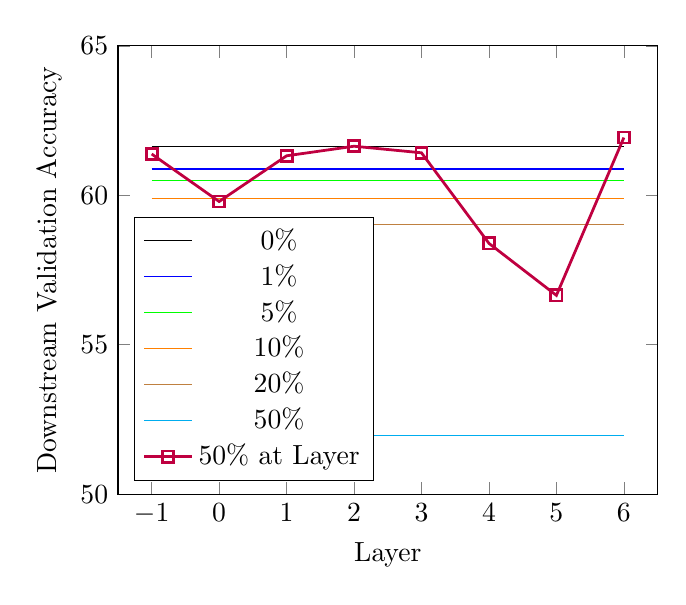
\begin{tikzpicture}
\begin{axis}[
    %title={Temperature dependence of CuSO\(_4\cdot\)5H\(_2\)O solubility},
    % width=0.8\textwidth,
    % height=0.5\textwidth,
    xlabel={Layer},
    ylabel={Downstream Validation Accuracy},
    xmin=-1.5, xmax=6.5,
    ymin=57, ymax=65,
    xtick={-1,0,1,2,3,4,5,6,7}, %,11,12,13},
    ymin=50, ymax=65,
    %ytick={51,52,53,54,55,56,57,58,59,60,61,62,63,64,65},
    ytick={50, 55, 60, 65}, % ,52,53,54,55,56,57,58,59,60,61,62,63,64,65},
    %ytick={0,0.2,0.4,0.6,0.8,1.0}, %,0.6,0.7,0.8,0.9,1.0},
    legend pos=south west,
    %ymajorgrids=true,
    %grid style=dashed,
]
\addplot[
    %dashed,
    mark options={solid},
    color=black,
    %mark=diamond,
    ]
    coordinates {
    % (300,62.14999771118164)(600,63.15999984741211)(900,62.91999816894531)(1200,62.29999923706055)(1500,61.93000030517578)
    (-1,61.64)
    (0,61.64)
    (1,61.64)
    (2,61.64)
    (3,61.64)
    (4,61.64)
    (5,61.64)
    (6,61.64)
    };
    \addlegendentry{0\%}
\addplot[
    %dashed,
    mark options={solid},
    color=blue,
    %mark=pentagon,
    ]
    coordinates {
    (-1, 60.87999725341797)
    (0, 60.87999725341797) 
    (1, 60.87999725341797)
    (2, 60.87999725341797)
    (3, 60.87999725341797)
    (4, 60.87999725341797)
    (5, 60.87999725341797)
    (6, 60.87999725341797)
    };
    \addlegendentry{1\%}
\addplot[
    %dashed,
    mark options={solid},
    color=green,
    %mark=triangle,
    ]
    coordinates {
    (-1, 60.5)
    (0, 60.5)
    (1, 60.5)
    (2, 60.5)
    (3, 60.5)
    (4, 60.5)
    (5, 60.5)
    (6, 60.5)
    };
    \addlegendentry{5\%}
\addplot[
    %dashed,
    mark options={solid},
    color=orange,
    %mark=o,
    ]
    coordinates {
    (-1, 59.87999725341797)
    (0, 59.87999725341797)
    (1, 59.87999725341797)
    (2, 59.87999725341797)
    (3, 59.87999725341797)
    (4, 59.87999725341797)
    (5, 59.87999725341797)
    (6, 59.87999725341797)
    };
    \addlegendentry{10\%}
\addplot[
    %dashed,
    mark options={solid},
    color=brown,
    %mark=diamond,
    ]
    coordinates {
    (-1, 59.0099983215332)
    (0, 59.0099983215332)
    (1, 59.0099983215332)
    (2, 59.0099983215332)
    (3, 59.0099983215332)
    (4, 59.0099983215332)
    (5, 59.0099983215332)
    (6, 59.0099983215332)
    };
    \addlegendentry{20\%}
\addplot[
    %dashed,
    mark options={solid},
    color=cyan,
    %mark=square,
    ]
    coordinates {
    (-1, 51.96999740600586)
    (0, 51.96999740600586)
    (1, 51.96999740600586)
    (2, 51.96999740600586)
    (3, 51.96999740600586)
    (4, 51.96999740600586)
    (5, 51.96999740600586)
    (6, 51.96999740600586)
    };
    \addlegendentry{50\%}

\addplot[
    % dashed,
    % mark options={solid},
    %very thick,
    line width=1pt,
    color=purple,
    mark=square,
    ]
    coordinates {
    (-1, 61.37999725341797)
    (0, 59.78999710083008)
    (1, 61.31999969482422)
    (2, 61.63999938964844)
    (3, 61.41999816894531)
    (4, 58.38999938964844)
    (5, 56.64999771118164)
    (6, 61.93000030517578) 
    };
    \addlegendentry{50\% at Layer}


\end{axis}
\end{tikzpicture}
}
\vspace{-.2in}
%\caption{Continue Cifar100-Cifar100}
\caption{Comparing dropout rates at all layers versus 50\% dropout rate targeted at a specific layer.\vspace{-.2in}}
\label{fig:cifar100-cifar100-drop-all-vs-layer}
%\vspace{-0.5cm}
\end{figure}



%%%%%%%%%%%%%%%%%%%%%%%%%%
% \begin{figure}
% \begin{subfigure}{.49\columnwidth}
% \centering
% \resizebox{\columnwidth}{!}{%
% }
% \end{subfigure}%
% \hspace{0.005\columnwidth}
% \begin{subfigure}{.49\columnwidth}
% \centering
% \resizebox{\columnwidth}{!}{%
% }
% \end{subfigure}
% \caption{A figure with two subfigures}
% \label{fig:test}
% \end{figure}
%%%%%%%%%%%%%%%%%%%%%%%%%%%%%%%%%%%

%In this work we are not interested in slight performance increases due to 1\% dropout, but rather the behavior of substantial dropout targeted at certain layers.
% \justin{Not sure about this:}T

We study the behavior of dropout targeted at certain layers. Thus, we use 50\% dropout that drastically reduced performance when applied at all layers, to see how performance changes when it is targeted at a single layer. 
In Figure \ref{fig:cifar100-cifar100-drop-all-vs-layer}, we see 50\% dropout applied at single layers. Downstream performance is clearly better, and certain layers perform on par with the benchmark and Layer 6 sightly outperforms it.

%\justin{compare to the same dropout rate?}

%but still only dropout at the last Layer 6 (which is in the final latent space) helps improve performance and is outperforming the best 1\% dropout in Figure \ref{fig:drop_everywhere_cifar100}. 

% \begin{figure}[ht]
% \centering

% %\vspace{-0.5cm}
% \end{figure}

Next, we apply Deep Augmentation to \emph{all samples} uniformly with stop-gradient before the targeted layer; since augmentation is applied to all data points, in effect, stop-gradient prevents lower layer weights from changing at all. Results are in the Appendix (Figure \ref{fig:two-sided-dropout-cifar100-cifar100}), but performance breaks down as we move to higher layers. This is likely due to: (1) as we move up layers we are training fewer parameters and leaving earlier layers fixed to random weights, and (2) all contrastive pairs are transformed at the same layer.

Contrastive learning aims to compare complementary perspectives. Therefore, it might be useful to provide pairs that contrast higher-layer transformations to input-data transformations. In addition, randomly perturbing higher layers is not representative of the data distribution  at test time. %all samples have higher transformations, and since those are not performed in downstream training and testing, we have created a training versus testing disparity. 

% In any event, in order to try to propagate the gradient below layers that are not targeted with transformations but still train the whole network, we need to only transform a random sample of examples in a batch

Addressing these points, we next augment only a random subset of each batch. We sample 50\% of each batch and perform a 50\% dropout; stop-gradient is applied only in that 50\%. The result can be found as ``Stop" in Figure \ref{fig:cifar100-cifar100-stop-vs-not}. 


% \begin{figure}
% \begin{subfigure}{.49\columnwidth}
% \resizebox{\columnwidth}{!}{%
% \begin{tikzpicture}
% \begin{axis}[
%     %title={Temperature dependence of CuSO\(_4\cdot\)5H\(_2\)O solubility},
%     % width=0.8\textwidth,
%     % height=0.5\textwidth,
%     xlabel={Num. Epochs Pre-training},
%     ylabel={Downstream Validation Accuracy},
%     xmin=230, xmax=1540,
%     ymin=57, ymax=65,
%     xtick={200,400,600,800,1000,1200,1400}, %,11,12,13},
%     ytick={57, 58, 59, 60, 61, 62, 63, 64, 65},
%     %ytick={0,0.2,0.4,0.6,0.8,1.0}, %,0.6,0.7,0.8,0.9,1.0},
%     legend pos=south west,
%     ymajorgrids=true,
%     grid style=dashed,
% ]
% \addplot[
%     color=black,
%     mark=diamond,
%     ]
%     coordinates {
%     (600,61.27)(900,61.78)(1200,61.76)(1500,61.64)
%     };
%     \addlegendentry{S}
% \addplot[
%     color=blue,
%     mark=square,
%     ]
%     coordinates {
%     (600,60.959999084472656)(900,62.39999771118164)(1200,61.12999725341797)(1500,61.43000030517578)
%     };
%     \addlegendentry{L-1}
% \addplot[
%     color=red,
%     mark=triangle,
%     ]
%     coordinates {
%     (600,60.62999725341797)(900,62.15999984741211)(1200,61.48999786376953)(1500,61.269996643066406)
%     };
%     \addlegendentry{L0}
% \addplot[
%     color=green,
%     mark=otimes,
%     ]
%     coordinates {
%     (600,61.1099967956543)(900,61.68000030517578)(1200,61.13999938964844)(1500,61.38999938964844)
%     };
%     \addlegendentry{L1}
% \addplot[
%     color=pink,
%     mark=square,
%     ]
%     coordinates {
%     (600,60.09000015258789)(900,60.54999923706055)(1200,61.06999969482422)(1500,61.94999694824219)
%     };
%     \addlegendentry{L2}
% \addplot[
%     color=orange,
%     mark=diamond,
%     ]
%     coordinates {
%     (600,57.41999816894531)(900,59.099998474121094)(1200,61.29999923706055)(1500,62.43000030517578)
%     };
%     \addlegendentry{L3}
% \addplot[
%     color=yellow,
%     mark=triangle,
%     ]
%     coordinates {
%     (600,59.96999740600586)(900,61.25)(1200,63.53999710083008)(1500,63.39999771118164)
%     };
%     \addlegendentry{L4}
% \addplot[
%     color=purple,
%     mark=otimes,
%     ]
%     coordinates {
%     (600,56.64999771118164)(900,57.21999740600586)(1200,58.689998626708984)(1500,58.59000015258789)
%     };
%     \addlegendentry{L5}
% \addplot[
%     color=teal,
%     mark=square,
%     ]
%     coordinates {
%     (600,58.209999084472656)(900,62.029998779296875)(1200,63.849998474121094)(1500,62.959999084472656)
%     };
%     \addlegendentry{L6}
% % \addplot[
% %     color=green,
% %     mark=square,
% %     ]
% %     coordinates {
% %     (300,55.84000015258789)(600,59.32999801635742)(900,61.41999816894531)(1200,62.869998931884766)(1500,63.56999969482422)
% %     };
% %     \addlegendentry{L4L6}

% % \addplot[
% %     color=brown,
% %     mark=square,
% %     ]
% %     coordinates {
% %     (300,56.28999710083008)(600,59.189998626708984)(900,62.6099967956543)(1200,62.82999801635742)(1500,62.89999771118164)
% %     };
% %     \addlegendentry{L4}

    

% \end{axis}
% \end{tikzpicture}
% %\vspace{-.1in}

% }
% \caption{With stop-gradient}
% \label{fig:cifar100-cifar100}
% \end{subfigure}%
% \hspace{0.005\columnwidth}
% \begin{subfigure}{.49\columnwidth}
% \centering
% \resizebox{\columnwidth}{!}{%
% \begin{tikzpicture}
% \begin{axis}[
%     %title={Temperature dependence of CuSO\(_4\cdot\)5H\(_2\)O solubility},
%     % width=0.8\textwidth,
%     % height=0.5\textwidth,
%     xlabel={Num. Epochs Pre-training},
%     ylabel={Downstream Validation Accuracy},
%     xmin=230, xmax=1540,
%     ymin=57, ymax=65,
%     xtick={200,400,600,800,1000,1200,1400}, %,11,12,13},
%     ytick={57, 58, 59, 60, 61, 62, 63, 64, 65},
%     %ytick={0,0.2,0.4,0.6,0.8,1.0}, %,0.6,0.7,0.8,0.9,1.0},
%     legend pos=south west,
%     ymajorgrids=true,
%     grid style=dashed,
% ]
% \addplot[
%     color=black,
%     mark=diamond,
%     ]
%     coordinates {
%     (600,61.27)(900,61.78)(1200,61.76)(1500,61.64)
%     };
%     \addlegendentry{S}
% \addplot[
%     color=blue,
%     mark=square,
%     ]
%     coordinates {
%     (600,60.959999084472656)(900,62.39999771118164)(1200,61.12999725341797)(1500,61.43000030517578)
%     };
%     \addlegendentry{L-1}
% \addplot[
%     color=red,
%     mark=triangle,
%     ]
%     coordinates {
%     (600,61.619998931884766)(900,62.269996643066406)(1200,62.099998474121094)(1500,62.029998779296875)
%     };
%     \addlegendentry{L0}
% \addplot[
%     color=green,
%     mark=otimes,
%     ]
%     coordinates {
%     (600,60.959999084472656)(900,62.69999694824219)(1200,61.37999725341797)(1500,62.13999938964844)
%     };
%     \addlegendentry{L1}
% \addplot[
%     color=pink,
%     mark=square,
%     ]
%     coordinates {
%     (600,61.019996643066406)(900,62.28999710083008)(1200,61.84000015258789)(1500,61.769996643066406)
%     };
%     \addlegendentry{L2}
% \addplot[
%     color=orange,
%     mark=diamond,
%     ]
%     coordinates {
%     (600,60.54999923706055)(900,62.119998931884766)(1200,61.32999801635742)(1500,61.07999801635742)
%     };
%     \addlegendentry{L3}
% \addplot[
%     color=yellow,
%     mark=triangle,
%     ]
%     coordinates {
%     (600,58.93000030517578)(900,59.89999771118164)(1200,59.91999816894531)(1500,59.519996643066406)
%     };
%     \addlegendentry{L4}
% \addplot[
%     color=purple,
%     mark=otimes,
%     ]
%     coordinates {
%     (600,57.84000015258789)(900,58.47999954223633)(1200,58.81999969482422)(1500,57.16999816894531)
%     };
%     \addlegendentry{L5}
% \addplot[
%     color=teal,
%     mark=square,
%     ]
%     coordinates {
%     (600,60.46999740600586)(900,62.09000015258789)(1200,62.72999954223633)(1500,61.73999786376953)
%     };
%     \addlegendentry{L6}

% % \addplot[
% %     color=teal,
% %     mark=square,
% %     ]
% %     coordinates {
% %     (300,58.599998474121094)(600,61.279998779296875)(900,62.62999725341797)(1200,62.14999771118164)(1500,61.91999816894531)
% %     };
% %     \addlegendentry{L6}

    

% \end{axis}
% \end{tikzpicture}
% %\vspace{-.1in}

% }
% %\vspace{-.1in}
% \caption{Without stop-gradient}
% \label{fig:trainble-cifar100-cifar100}
% \end{subfigure}
% \caption{Comparing sampling 50\% and apply 50\% dropout, with or without stop-gradient.}
% \label{fig:test}
% \end{figure}




\begin{figure}[ht]
\centering
\resizebox{1.0\columnwidth}{!}{%
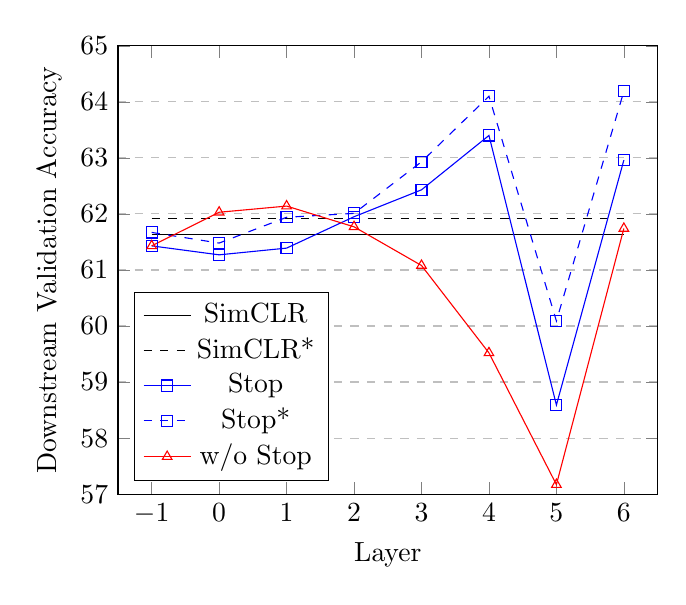
\begin{tikzpicture}
\begin{axis}[
    %title={Temperature dependence of CuSO\(_4\cdot\)5H\(_2\)O solubility},
    % width=0.8\textwidth,
    % height=0.5\textwidth,
    xlabel={Layer},
    ylabel={Downstream Validation Accuracy},
    xmin=-1.5, xmax=6.5,
    ymin=57, ymax=65,
    xtick={-1,0,1,2,3,4,5,6,7}, %,11,12,13},
    ytick={57, 58, 59, 60, 61, 62, 63, 64, 65},
    %ytick={0,0.2,0.4,0.6,0.8,1.0}, %,0.6,0.7,0.8,0.9,1.0},
    legend pos=south west,
    ymajorgrids=true,
    grid style=dashed,
]
\addplot[
    color=black,
    %mark=diamond,
    ]
    coordinates {
    % (300,62.14999771118164)(600,63.15999984741211)(900,62.91999816894531)(1200,62.29999923706055)(1500,61.93000030517578)
    (-1,61.64)
    (0,61.64)
    (1,61.64)
    (2,61.64)
    (3,61.64)
    (4,61.64)
    (5,61.64)
    (6,61.64)
    };
    \addlegendentry{SimCLR}
\addplot[
    %dotted,
    dashed,
    mark options={solid},
    color=black,
    %mark=diamond,
    ]
    coordinates {
    % (300,62.14999771118164)(600,63.15999984741211)(900,62.91999816894531)(1200,62.29999923706055)(1500,61.93000030517578)
    (-1,61.91999816894531)
    (0,61.91999816894531)
    (1,61.91999816894531)
    (2,61.91999816894531)
    (3,61.91999816894531)
    (4,61.91999816894531)
    (5,61.91999816894531)
    (6,61.91999816894531)
    };
    \addlegendentry{SimCLR*}
\addplot[
    color=blue,
    mark=square,
    ]
    coordinates {
    (-1, 61.43000030517578)
    (0, 61.269996643066406) 
    (1, 61.38999938964844)
    (2, 61.94999694824219)
    (3, 62.43000030517578)
    (4, 63.39999771118164)
    (5, 58.59000015258789)
    (6, 62.959999084472656)
    };
    \addlegendentry{Stop}
\addplot[
    dashed,
    mark options={solid},
    color=blue,
    mark=square,
    ]
    coordinates {
    (-1, 61.66999816894531)
    (0, 61.47999954223633)
    (1, 61.939998626708984)
    (2, 62.0099983215332)
    (3, 62.93000030517578)
    (4, 64.0999984741211)
    (5, 60.09000015258789)
    (6, 64.18999481201172)
    };
    \addlegendentry{Stop*}
\addplot[
    color=red,
    mark=triangle,
    ]
    coordinates {
    (-1, 61.43000030517578)
    (0, 62.029998779296875)
    (1, 62.13999938964844)
    (2, 61.769996643066406)
    (3, 61.07999801635742)
    (4, 59.519996643066406)
    (5, 57.16999816894531)
    (6, 61.73999786376953)
    };
    \addlegendentry{w/o Stop}
% \addplot[
%     dashed,
%     mark options={solid},
%     color=red,
%     mark=triangle,
%     ]
%     coordinates {
%     (-1, 61.66999816894531)
%     (0, 61.59000015258789)
%     (1, 61.55999755859375)
%     (2, 61.849998474121094)
%     (3, 62.21999740600586)
%     (4, 59.62999725341797)
%     (5, 58.68000030517578)
%     (6, 61.5099983215332)
%     };
%     \addlegendentry{w/o Stop*}


\end{axis}
\end{tikzpicture}
}
\vspace{-.2in}
%\caption{Continue Cifar100-Cifar100}
\caption{Comparing sampling 50\% of batch and applying 50\% dropout rate to that sample, with and without stop-gradient. *: initialized with pre-trained SimCLR model. ``Stop" is short for stop-gradient.\vspace{-.2in}}
\label{fig:cifar100-cifar100-stop-vs-not}
%\vspace{-0.5cm}
\end{figure}



This strategy yields significant performance gains. Deep Augmentation with stop-gradient at Layer 6 (the final latent space) and Layer 4 stand out, but also other layers outperform SimCLR. Interestingly, Layer 4 is the second worst performing layer in Figure \ref{fig:cifar100-cifar100-drop-all-vs-layer} where stop-gradient is not used, but now it performs well. Since we randomly transform 50\% of the batch, on average 25\% of contrasted pairs will both have higher-layer transformations, 25\% will have no higher-layer transformations (just SimCLR), and 50\% will contrast higher-layer transformations with input data transformations. 

To fairly compare Deep Augmentaion with and without stop-gradient, and to assert that the difference is not only due to these two new types of contrasting pairs (higher-to-data and data-to-data) but also to stop-gradient, we now train using an identical setup as ``Stop" in Figure \ref{fig:cifar100-cifar100-stop-vs-not} but without the stop-gradient. In other words, we randomly sample 50\% of the batch and apply 50\% dropout at a targeted layer without stop-gradient; results are labeled ``w/o Stop" in Figure \ref{fig:cifar100-cifar100-stop-vs-not}. There is now some improvement compared to SimCLR: targeting layers 0 and 1 increases performance. Layers 0 and 1 perform dropout just after the first and second layers in ResNet18, resp.; thus, performance compared to applying dropout to \emph{all} samples is improved when early layers do not always experience drastic dropout. This may be due to less flexibility of early layers as they have fewer parameters at their disposal, compared to higher layers; see the Appendix for discussion.
%\justin{try again or remove; make it short} {\color{red} Early layers have fewer parameters to learn to be invariant to these transformations with respect to non-augmented images. This fools the network into believing the data-distribution is different from how it actually looks like at test time; the NN effectively never sees non-augmented data during training, and dropout is not creating realistic looking images as opposed to typical image transformations like cropping.}

% \begin{figure}[ht]
% \centering
% \begin{tikzpicture}
% \begin{axis}[
%     %title={Temperature dependence of CuSO\(_4\cdot\)5H\(_2\)O solubility},
%     % width=0.8\textwidth,
%     % height=0.5\textwidth,
%     xlabel={Num. Epochs Pre-training},
%     ylabel={Downstream Validation Accuracy},
%     xmin=230, xmax=1540,
%     ymin=57, ymax=65,
%     xtick={200,400,600,800,1000,1200,1400}, %,11,12,13},
%     ytick={57, 58, 59, 60, 61, 62, 63, 64, 65},
%     %ytick={0,0.2,0.4,0.6,0.8,1.0}, %,0.6,0.7,0.8,0.9,1.0},
%     legend pos=south west,
%     ymajorgrids=true,
%     grid style=dashed,
% ]
% \addplot[
%     color=black,
%     mark=diamond,
%     ]
%     coordinates {
%     (600,61.27)(900,61.78)(1200,61.76)(1500,61.64)
%     };
%     \addlegendentry{S}
% \addplot[
%     color=blue,
%     mark=square,
%     ]
%     coordinates {
%     (600,60.959999084472656)(900,62.39999771118164)(1200,61.12999725341797)(1500,61.43000030517578)
%     };
%     \addlegendentry{L-1}
% \addplot[
%     color=red,
%     mark=triangle,
%     ]
%     coordinates {
%     (600,61.619998931884766)(900,62.269996643066406)(1200,62.099998474121094)(1500,62.029998779296875)
%     };
%     \addlegendentry{L0}
% \addplot[
%     color=green,
%     mark=otimes,
%     ]
%     coordinates {
%     (600,60.959999084472656)(900,62.69999694824219)(1200,61.37999725341797)(1500,62.13999938964844)
%     };
%     \addlegendentry{L1}
% \addplot[
%     color=pink,
%     mark=square,
%     ]
%     coordinates {
%     (600,61.019996643066406)(900,62.28999710083008)(1200,61.84000015258789)(1500,61.769996643066406)
%     };
%     \addlegendentry{L2}
% \addplot[
%     color=orange,
%     mark=diamond,
%     ]
%     coordinates {
%     (600,60.54999923706055)(900,62.119998931884766)(1200,61.32999801635742)(1500,61.07999801635742)
%     };
%     \addlegendentry{L3}
% \addplot[
%     color=yellow,
%     mark=triangle,
%     ]
%     coordinates {
%     (600,58.93000030517578)(900,59.89999771118164)(1200,59.91999816894531)(1500,59.519996643066406)
%     };
%     \addlegendentry{L4}
% \addplot[
%     color=purple,
%     mark=otimes,
%     ]
%     coordinates {
%     (600,57.84000015258789)(900,58.47999954223633)(1200,58.81999969482422)(1500,57.16999816894531)
%     };
%     \addlegendentry{L5}
% \addplot[
%     color=teal,
%     mark=square,
%     ]
%     coordinates {
%     (600,60.46999740600586)(900,62.09000015258789)(1200,62.72999954223633)(1500,61.73999786376953)
%     };
%     \addlegendentry{L6}

% % \addplot[
% %     color=teal,
% %     mark=square,
% %     ]
% %     coordinates {
% %     (300,58.599998474121094)(600,61.279998779296875)(900,62.62999725341797)(1200,62.14999771118164)(1500,61.91999816894531)
% %     };
% %     \addlegendentry{L6}

    

% \end{axis}
% \end{tikzpicture}
% %\vspace{-.1in}
% \caption{Trainable Cifar100-Cifar100}
% \label{fig:trainble-cifar100-cifar100}
% %\vspace{-0.5cm}
% \end{figure}

 Comparing ``Stop" and ``w/o Stop" in Figure \ref{fig:cifar100-cifar100-stop-vs-not}, the downstream performance of Layers 4, 3, and 6 greatly benefits from stop-gradient. %This indicates that there is a real difference between Deep Augmentation with and without the stop-gradient.
%and interesting to know if it's due to the duplication of information that might occur then stop-gradient is not used. 


We also assess the domain transfer performance by evaluating the networks pre-trained on CIFAR100 on the downstream task of CIFAR10. In this case, stop-gradient also generally performs better than without stop-gradient, especially in Layers 3 and 4, and substantially outperforms SimCLR; see the  Appendix for details.

\subsubsection{Initialization and Freezing Weights}
\label{sec:Initialization-and-Freezing-Weights}

Higher-layer augmentations may be more interesting when the network already has learned useful and discriminative features up to those layers. Furthermore, the simultaneous learning of features and being invariant to their corruption might become opposing objectives, slowing down training or making it unstable. Thus, we apply Deep Augmentation to a NN that has already been trained using SimCLR. Results for Deep Augmentation with stop-gradient using this initialization are labeled ``Stop*" in Figure \ref{fig:cifar100-cifar100-stop-vs-not}. At several layers, Deep Augmentation benefits more than the ``SimCLR*" baseline (SimCLR trained twice). In addition, the trends across layers are the same as ``Stop" with random initialization. 

% \begin{figure}[ht]
% \centering
% \resizebox{0.8\columnwidth}{!}{%
% \begin{tikzpicture}
% \begin{axis}[
%     %title={Temperature dependence of CuSO\(_4\cdot\)5H\(_2\)O solubility},
%     % width=0.8\textwidth,
%     % height=0.5\textwidth,
%     xlabel={Num. Epochs Pre-training},
%     ylabel={Downstream Validation Accuracy},
%     xmin=230, xmax=1540,
%     ymin=57, ymax=65,
%     xtick={200,400,600,800,1000,1200,1400}, %,11,12,13},
%     ytick={57, 58, 59, 60, 61, 62, 63, 64, 65},
%     %ytick={0,0.2,0.4,0.6,0.8,1.0}, %,0.6,0.7,0.8,0.9,1.0},
%     legend pos=south west,
%     ymajorgrids=true,
%     grid style=dashed,
% ]
% \addplot[
%     color=black,
%     mark=diamond,
%     ]
%     coordinates {
%     % (300,62.14999771118164)(600,63.15999984741211)(900,62.91999816894531)(1200,62.29999923706055)(1500,61.93000030517578)
%     (300,62.79999923706055)(600,62.5)(900,62.87999725341797)(1200,62.28999710083008)(1500,61.91999816894531)
%     };
%     \addlegendentry{S}
% \addplot[
%     color=blue,
%     mark=square,
%     ]
%     coordinates {
%     (600,61.94999694824219)(900,62.209999084472656)(1200,61.939998626708984)(1500,61.66999816894531)
%     %(300,60.39999771118164)(600,61.98999786376953)(900,62.3599967956543)(1200,61.73999786376953)(1500,61.7599983215332)
%     };
%     \addlegendentry{L-1}
% \addplot[
%     color=red,
%     mark=triangle,
%     ]
%     coordinates {
%     (600,62.12999725341797)(900,62.13999938964844)(1200,61.619998931884766)(1500,61.47999954223633)
%     %(300,60.779998779296875)(600,61.3599967956543)(900,62.15999984741211)(1200,61.119998931884766)(1500,60.91999816894531)
%     };
%     \addlegendentry{L0}
% \addplot[
%     color=green,
%     mark=otimes,
%     ]
%     coordinates {
%     (600,61.5099983215332)(900,62.209999084472656)(1200,62.3599967956543)(1500,61.939998626708984)
%     %(300,60.119998931884766)(600,61.30999755859375)(900,62.769996643066406)(1200,61.619998931884766)(1500,61.80999755859375)
%     };
    
%     \addlegendentry{L1}
% \addplot[
%     color=pink,
%     mark=square,
%     ]
%     coordinates {
%     (300,59.72999954223633)(600,60.269996643066406)(900,61.14999771118164)(1200,61.44999694824219)(1500,62.0099983215332)
%     %(300,59.72999954223633)(600,60.269996643066406)(900,61.14999771118164)(1200,61.44999694824219)(1500,62.0099983215332)
%     };
%     \addlegendentry{L2}
% \addplot[
%     color=orange,
%     mark=diamond,
%     ]
%     coordinates {
%     (300,57.94999694824219)(600,58.459999084472656)(900,60.71999740600586)(1200,62.75)(1500,62.93000030517578)
%     };
%     \addlegendentry{L3}
% \addplot[
%     color=yellow,
%     mark=triangle,
%     ]
%     coordinates {
%     (300,59.869998931884766)(600,61.72999954223633)(900,62.2599983215332)(1200,64.22000122070312)(1500,64.0999984741211)
%     };
%     \addlegendentry{L4}
% \addplot[
%     color=purple,
%     mark=otimes,
%     ]
%     coordinates {
%     (300,58.07999801635742)(600,58.869998931884766)(900,59.869998931884766)(1200,60.18000030517578)(1500,60.09000015258789)
%     };
%     \addlegendentry{L5}
% \addplot[
%     color=teal,
%     mark=square,
%     ]
%     coordinates {
%     (300,59.63999938964844)(600,60.80999755859375)(900,62.57999801635742)(1200,64.29000091552734)(1500,64.18999481201172)
%     };
%     \addlegendentry{L6}

% \end{axis}
% \end{tikzpicture}
% }
% %\vspace{-.1in}
% %\caption{Continue Cifar100-Cifar100}
% \caption{50\% sampling, 50\% dropout, with stop-gradient, and initialized with pre-trained SimCLR model.}
% \label{fig:continue-cifar100-cifar100}
% %\vspace{-0.5cm}
% \end{figure}

This experiment indicates that the effectiveness of higher-layer transformations is not dependent on first training with SimCLR---not even for deeper layers. This suggests that the layers before the targeted layer benefit from diverging from the features of SimCLR alone.
%and it is a better use of those parameters



Finally, we repeat the experiment with pre-trained initialization but freeze all the layers up to and including the layer at which the targeted transformation occurs; see ``Freeze before" in Figure \ref{fig:cifar100-cifar100-freeze}. Compared to not freezing, this strategy gives very different results. In particular, the downstream performance of Layers 3 and 4 is critically reduced. %; note that Layer 6 means freezing the whole NN. 

%We note in Appendix, Layer 1 and Layer 2 performance is significantly improved and show stronger performance than the SimCLR benchmark in earlier epochs until it shows overfitting behavior. This indicates that there is room to learn improved representation by learning invariances of higher layer SimCLR feature spaces. Future work may explore an iterative approach where we incrementally freeze layers, moving one step up at a time.

%\justin{We got here.}


Deep Augmentation after frozen SimCLR layers may not work well due to co-adaptation between neurons, leading to overfitting. Suppose a layer of a NN exhibits strong co-adaptation within several subsets of neurons, i.e., each subset encodes a single data feature. Randomly dropping neurons is unlikely to remove a complete co-adapted subset of neurons. Ideally, features are learned per neuron so dropping any of them provides a complementary view. Alternatively, features might be represented continuously among neurons in a layer such that dropout corresponds to something akin to blurring the feature continuously.
%, again providing complementary rather than supplementary views. 

%{\color{red} 
Because early layers have fewer parameters to distort the input data, such layers may have less co-adaptation.
%---especially in CNNs where there is a strong inductive image-bias. 
This might explain why earlier layers, rather than later layers, perform better when frozen during Deep Augmentation. Similarly, higher layers may benefit from higher dropout rates because they are more susceptible to co-adaptation, explaining why in Figure \ref{fig:cifar100-cifar100-stop-vs-not}, Deep Augmentation in higher layers yields the best downstream performance. See Appendix \ref{appendix:freezing-layers} for further discussion. 
%Either way, training a NN with dropout should lead to less co-adaptation and in turn make higher layer transformations more useful. 
%This logic suggests that a NN trained with Deep Augmentation at a certain layer may be suitable for further training on a new dataset (optionally frozen up to that layer) using Deep Augmentation at the same layer.
%Future work may investigate ways to optimally train a NN so that dropout serves as a useful higher transformation. 
%}

Reversely, we may freeze the layers following the targeted layer; results are labeled ``Freeze after" in Figure \ref{fig:cifar100-cifar100-freeze}. Compared to ``Freeze before", Layer 3 improves, Layer 5 worsens, while Layer 4 performs similarly. This asserts that later layers, some more than others, benefit from learning to be invariant to Deep Augmentation. 
%\justin{Say something.}

%Either way, training a NN with dropout should lead to less co-adaptation and in turn that freezing and keep training with higher layer transformations more useful. Future work may investigate how to optimally train a NN so that dropout serves as a useful higher transformation.

% \begin{figure}
% \centering
% \begin{minipage}{.5\columnwidth}
%   \centering
%   \includegraphics[width=.4\linewidth]{images/Bars1.png}
%   \caption{A figure} % of{figure}{A figure}
%   \label{fig:test1}
% \end{minipage}%
% \begin{minipage}{.5\columnwidth}
%   \centering
%   \includegraphics[width=.4\linewidth]{images/Bars1.png}
%   %\captionof{figure}{Another figure}
%   \caption{A figure}
%   \label{fig:test2}
% \end{minipage}
% \end{figure}

% \begin{figure}
% \begin{minipage}{.49\columnwidth}
%   \centering
%   \resizebox{1.0\columnwidth}{!}{
% \centering
% \begin{tikzpicture}
% \begin{axis}[
%     %title={Temperature dependence of CuSO\(_4\cdot\)5H\(_2\)O solubility},
%     % width=0.8\textwidth,
%     % height=0.5\textwidth,
%     xlabel={Num. Epochs Pre-training},
%     ylabel={Downstream Validation Accuracy},
%     xmin=230, xmax=1540,
%     ymin=57, ymax=65,
%     xtick={200,400,600,800,1000,1200,1400}, %,11,12,13},
%     ytick={57, 58, 59, 60, 61, 62, 63, 64, 65},
%     %ytick={0,0.2,0.4,0.6,0.8,1.0}, %,0.6,0.7,0.8,0.9,1.0},
%     legend pos=south west,
%     ymajorgrids=true,
%     grid style=dashed,
% ]
% \addplot[
%     color=black,
%     mark=diamond,
%     ]
%     coordinates {
%     (300,62.79999923706055)(600,62.5)(900,62.87999725341797)(1200,62.28999710083008)(1500,61.91999816894531)
%     };
%     \addlegendentry{S}
% \addplot[
%     color=blue,
%     mark=square,
%     ]
%     coordinates {
%     (600,61.94999694824219)(900,62.209999084472656)(1200,61.939998626708984)(1500,61.66999816894531)
%     %(300,60.39999771118164)(600,61.98999786376953)(900,62.3599967956543)(1200,61.73999786376953)(1500,61.7599983215332)
%     };
%     \addlegendentry{L-1}
% \addplot[
%     color=red,
%     mark=triangle,
%     ]
%     coordinates {
%     (300,62.189998626708984)(600,62.2599983215332)(900,61.98999786376953)(1200,62.07999801635742)(1500,61.38999938964844)
%     %(300,61.03999710083008)(600,62.3599967956543)(900,62.1099967956543)(1200,62.43000030517578)(1500,61.769996643066406)
%     };
%     \addlegendentry{L0}
% \addplot[
%     color=green,
%     mark=otimes,
%     ]
%     coordinates {
%     (300,61.81999969482422)(600,62.94999694824219)(900,63.56999969482422)(1200,62.25)(1500,61.779998779296875)
%     %(300,62.28999710083008)(600,62.869998931884766)(900,63.439998626708984)(1200,63.09000015258789)(1500,62.0099983215332)
%     };
%     \addlegendentry{L1}
% \addplot[
%     color=pink,
%     mark=square,
%     ]
%     coordinates {
%     (300,61.869998931884766)(600,63.279998779296875)(900,63.69999694824219)(1200,62.03999710083008)(1500,61.54999923706055)
%     %(300,62.16999816894531)(600,62.959999084472656)(900,62.21999740600586)(1200,61.459999084472656)(1500,61.40999984741211)
%     };
%     \addlegendentry{L2}
% \addplot[
%     color=orange,
%     mark=diamond,
%     ]
%     coordinates {
%     (300,55.57999801635742)(600,55.46999740600586)(900,57.29999923706055)(1200,57.69999694824219)(1500,58.21999740600586)
%     };
%     \addlegendentry{L3}
% \addplot[
%     color=yellow,
%     mark=triangle,
%     ]
%     coordinates {
%     (300,59.97999954223633)(600,59.22999954223633)(900,60.439998626708984)(1200,60.79999923706055)(1500,61.209999084472656)
%     };
%     \addlegendentry{L4}
% \addplot[
%     color=purple,
%     mark=otimes,
%     ]
%     coordinates {
%     (300,59.30999755859375)(600,59.349998474121094)(900,59.84000015258789)(1200,60.90999984741211)(1500,61.349998474121094)
%     };
%     \addlegendentry{L5}
% % \addplot[
% %     color=teal,
% %     mark=square,
% %     ]
% %     coordinates {
% %     (300,59.599998474121094)(600,59.28999710083008)(900,60.30999755859375)(1200,60.63999938964844)(1500,61.07999801635742)
% %     % (300,59.63999938964844)(600,60.80999755859375)(900,62.57999801635742)(1200,64.29000091552734)(1500,64.18999481201172)
% %     };
% %     \addlegendentry{25}

% \end{axis}
% \end{tikzpicture}
% }
% %\vspace{-.1in}
% \caption{Freeze Continue Cifar100-Cifar100}
% \label{fig:freeze-continue-cifar100-cifar100}
% \end{minipage}%
% \hspace{.01\columnwidth}
% \begin{minipage}{.49\columnwidth}
%   \resizebox{1.0\columnwidth}{!}{
% \centering
% \begin{tikzpicture}
% \begin{axis}[
%     %title={Temperature dependence of CuSO\(_4\cdot\)5H\(_2\)O solubility},
%     % width=0.8\textwidth,
%     % height=0.5\textwidth,
%     xlabel={Num. Epochs Pre-training},
%     ylabel={Downstream Validation Accuracy},
%     xmin=230, xmax=1540,
%     ymin=57, ymax=65,
%     xtick={200,400,600,800,1000,1200,1400}, %,11,12,13},
%     ytick={57, 58, 59, 60, 61, 62, 63, 64, 65},
%     %ytick={0,0.2,0.4,0.6,0.8,1.0}, %,0.6,0.7,0.8,0.9,1.0},
%     legend pos=south west,
%     ymajorgrids=true,
%     grid style=dashed,
% ]
% \addplot[
%     color=black,
%     mark=diamond,
%     ]
%     coordinates {
%     (300,62.79999923706055)(600,62.5)(900,62.87999725341797)(1200,62.28999710083008)(1500,61.91999816894531)
%     };
%     \addlegendentry{S}
% % \addplot[
% %     color=blue,
% %     mark=square,
% %     ]
% %     coordinates {
% %     (600,61.94999694824219)(900,62.209999084472656)(1200,61.939998626708984)(1500,61.66999816894531)
% %     };
% %     \addlegendentry{L-1}
% \addplot[
%     color=red,
%     mark=triangle,
%     ]
%     coordinates {
%     (300,58.37999725341797)(600,58.30999755859375)(900,58.64999771118164)(1200,59.80999755859375)(1500,60.369998931884766)
%     };
%     \addlegendentry{L0}
% \addplot[
%     color=green,
%     mark=otimes,
%     ]
%     coordinates {
%     (300,59.38999938964844)(600,59.019996643066406)(900,59.8599967956543)(1200,60.28999710083008)(1500,61.3599967956543)
%     };
%     \addlegendentry{L1}
% \addplot[
%     color=pink,
%     mark=square,
%     ]
%     coordinates {
%     (300,58.68000030517578)(600,59.1099967956543)(900,60.16999816894531)(1200,61.06999969482422)(1500,61.90999984741211)
%     };
%     \addlegendentry{L2}
% \addplot[
%     color=orange,
%     mark=diamond,
%     ]
%     coordinates {
%     (300,58.519996643066406)(600,60.34000015258789)(900,59.689998626708984)(1200,61.209999084472656)(1500,61.69999694824219)
%     };
%     \addlegendentry{L3}
% \addplot[
%     color=yellow,
%     mark=triangle,
%     ]
%     coordinates {
%     (300,59.32999801635742)(600,60.05999755859375)(900,61.38999938964844)(1200,60.25)(1500,60.6099967956543)
%     };
%     \addlegendentry{L4}
% \addplot[
%     color=purple,
%     mark=otimes,
%     ]
%     coordinates {
%     (300,56.07999801635742)(600,56.53999710083008)(900,57.7599983215332)(1200,57.57999801635742)(1500,56.81999969482422)
%     };
%     \addlegendentry{L5}
% % \addplot[
% %     color=teal,
% %     mark=square,
% %     ]
% %     coordinates {
% %     (300,61.63999938964844)(600,61.97999954223633)(900,62.91999816894531)(1200,62.62999725341797)(1500,61.5099983215332)
% %     };
% %     \addlegendentry{L6}

% \end{axis}
% \end{tikzpicture}
% }
% %\vspace{-.1in}
% \caption{Continue Freeze Reverse Cifar100-Cifar100}
% \label{fig:freeze-reverse-continue-cifar100-cifar100}

% \end{minipage}
% \end{figure}


% \begin{figure}
% \begin{subfigure}{.49\columnwidth}
%   \centering
%   \resizebox{1.0\columnwidth}{!}{
%   \begin{tikzpicture}
% \begin{axis}[
%     %title={Temperature dependence of CuSO\(_4\cdot\)5H\(_2\)O solubility},
%     % width=0.8\textwidth,
%     % height=0.5\textwidth,
%     xlabel={Num. Epochs Pre-training},
%     ylabel={Downstream Validation Accuracy},
%     xmin=230, xmax=1540,
%     ymin=57, ymax=65,
%     xtick={200,400,600,800,1000,1200,1400}, %,11,12,13},
%     ytick={57, 58, 59, 60, 61, 62, 63, 64, 65},
%     %ytick={0,0.2,0.4,0.6,0.8,1.0}, %,0.6,0.7,0.8,0.9,1.0},
%     legend pos=south west,
%     ymajorgrids=true,
%     grid style=dashed,
% ]
% \addplot[
%     color=black,
%     mark=diamond,
%     ]
%     coordinates {
%     (300,62.79999923706055)(600,62.5)(900,62.87999725341797)(1200,62.28999710083008)(1500,61.91999816894531)
%     };
%     \addlegendentry{S}
% \addplot[
%     color=blue,
%     mark=square,
%     ]
%     coordinates {
%     (600,61.94999694824219)(900,62.209999084472656)(1200,61.939998626708984)(1500,61.66999816894531)
%     %(300,60.39999771118164)(600,61.98999786376953)(900,62.3599967956543)(1200,61.73999786376953)(1500,61.7599983215332)
%     };
%     \addlegendentry{L-1}
% \addplot[
%     color=red,
%     mark=triangle,
%     ]
%     coordinates {
%     (300,62.189998626708984)(600,62.2599983215332)(900,61.98999786376953)(1200,62.07999801635742)(1500,61.38999938964844)
%     %(300,61.03999710083008)(600,62.3599967956543)(900,62.1099967956543)(1200,62.43000030517578)(1500,61.769996643066406)
    
%     };
%     \addlegendentry{L0}
% \addplot[
%     color=green,
%     mark=otimes,
%     ]
%     coordinates {
%     (300,61.81999969482422)(600,62.94999694824219)(900,63.56999969482422)(1200,62.25)(1500,61.779998779296875)
%     %(300,62.28999710083008)(600,62.869998931884766)(900,63.439998626708984)(1200,63.09000015258789)(1500,62.0099983215332)
    
%     };
%     \addlegendentry{L1}
% \addplot[
%     color=pink,
%     mark=square,
%     ]
%     coordinates {
%     (300,61.869998931884766)(600,63.279998779296875)(900,63.69999694824219)(1200,62.03999710083008)(1500,61.54999923706055)
%     %(300,62.16999816894531)(600,62.959999084472656)(900,62.21999740600586)(1200,61.459999084472656)(1500,61.40999984741211)
    
%     };
%     \addlegendentry{L2}
% \addplot[
%     color=orange,
%     mark=diamond,
%     ]
%     coordinates {
%     (300,55.57999801635742)(600,55.46999740600586)(900,57.29999923706055)(1200,57.69999694824219)(1500,58.21999740600586)
    
%     };
%     \addlegendentry{L3}
% \addplot[
%     color=yellow,
%     mark=triangle,
%     ]
%     coordinates {
%     (300,59.97999954223633)(600,59.22999954223633)(900,60.439998626708984)(1200,60.79999923706055)(1500,61.209999084472656)
    
%     };
%     \addlegendentry{L4}
% \addplot[
%     color=purple,
%     mark=otimes,
%     ]
%     coordinates {
%     (300,59.30999755859375)(600,59.349998474121094)(900,59.84000015258789)(1200,60.90999984741211)(1500,61.349998474121094)
    
%     };
%     \addlegendentry{L5}
% % \addplot[
% %     color=teal,
% %     mark=square,
% %     ]
% %     coordinates {
% %     (300,59.599998474121094)(600,59.28999710083008)(900,60.30999755859375)(1200,60.63999938964844)(1500,61.07999801635742)
% %     % (300,59.63999938964844)(600,60.80999755859375)(900,62.57999801635742)(1200,64.29000091552734)(1500,64.18999481201172)
% %     };
% %     \addlegendentry{25}

% \end{axis}
% \end{tikzpicture}
% }
% %\caption{Freeze Continue Cifar100-Cifar100}
% \caption{Freeze layers before Deep Augmentation}
% \label{fig:freeze-continue-cifar100-cifar100}
% \end{subfigure}%
% \hspace{0.005\columnwidth}
% \begin{subfigure}{.49\columnwidth}
%   \centering
%   \resizebox{1.0\columnwidth}{!}{
% \centering
% \begin{tikzpicture}
% \begin{axis}[
%     %title={Temperature dependence of CuSO\(_4\cdot\)5H\(_2\)O solubility},
%     % width=0.8\textwidth,
%     % height=0.5\textwidth,
%     xlabel={Num. Epochs Pre-training},
%     ylabel={Downstream Validation Accuracy},
%     xmin=230, xmax=1540,
%     ymin=57, ymax=65,
%     xtick={200,400,600,800,1000,1200,1400}, %,11,12,13},
%     ytick={57, 58, 59, 60, 61, 62, 63, 64, 65},
%     %ytick={0,0.2,0.4,0.6,0.8,1.0}, %,0.6,0.7,0.8,0.9,1.0},
%     legend pos=south west,
%     ymajorgrids=true,
%     grid style=dashed,
% ]
% \addplot[
%     color=black,
%     mark=diamond,
%     ]
%     coordinates {
%     (300,62.79999923706055)(600,62.5)(900,62.87999725341797)(1200,62.28999710083008)(1500,61.91999816894531)
%     };
%     \addlegendentry{S}
% % \addplot[
% %     color=blue,
% %     mark=square,
% %     ]
% %     coordinates {
% %     (600,61.94999694824219)(900,62.209999084472656)(1200,61.939998626708984)(1500,61.66999816894531)
% %     };
% %     \addlegendentry{L-1}
% \addplot[
%     color=red,
%     mark=triangle,
%     ]
%     coordinates {
%     (300,58.37999725341797)(600,58.30999755859375)(900,58.64999771118164)(1200,59.80999755859375)(1500,60.369998931884766)
%     };
%     \addlegendentry{L0}
% \addplot[
%     color=green,
%     mark=otimes,
%     ]
%     coordinates {
%     (300,59.38999938964844)(600,59.019996643066406)(900,59.8599967956543)(1200,60.28999710083008)(1500,61.3599967956543)
%     };
%     \addlegendentry{L1}
% \addplot[
%     color=pink,
%     mark=square,
%     ]
%     coordinates {
%     (300,58.68000030517578)(600,59.1099967956543)(900,60.16999816894531)(1200,61.06999969482422)(1500,61.90999984741211)
%     };
%     \addlegendentry{L2}
% \addplot[
%     color=orange,
%     mark=diamond,
%     ]
%     coordinates {
%     (300,58.519996643066406)(600,60.34000015258789)(900,59.689998626708984)(1200,61.209999084472656)(1500,61.69999694824219)
%     };
%     \addlegendentry{L3}
% \addplot[
%     color=yellow,
%     mark=triangle,
%     ]
%     coordinates {
%     (300,59.32999801635742)(600,60.05999755859375)(900,61.38999938964844)(1200,60.25)(1500,60.6099967956543)
%     };
%     \addlegendentry{L4}
% \addplot[
%     color=purple,
%     mark=otimes,
%     ]
%     coordinates {
%     (300,56.07999801635742)(600,56.53999710083008)(900,57.7599983215332)(1200,57.57999801635742)(1500,56.81999969482422)
    
    
%     };
%     \addlegendentry{L5}
% % \addplot[
% %     color=teal,
% %     mark=square,
% %     ]
% %     coordinates {
% %     (300,61.63999938964844)(600,61.97999954223633)(900,62.91999816894531)(1200,62.62999725341797)(1500,61.5099983215332)
% %     };
% %     \addlegendentry{L6}

% \end{axis}
% \end{tikzpicture}
% }
% %\vspace{-.1in}
% %\caption{Continue Freeze Reverse Cifar100-Cifar100}
% \caption{Freeze layers after Deep Augmentation}
% \label{fig:freeze-reverse-continue-cifar100-cifar100}
% \end{subfigure}
% \caption{Comparing freezing layers before or after Deep Augmentation with stop-gradient initialized with pre-trained SimCLR model.}
% \label{fig:test}
% \end{figure}


\begin{figure}[ht]
\centering
\resizebox{1.0\columnwidth}{!}{%
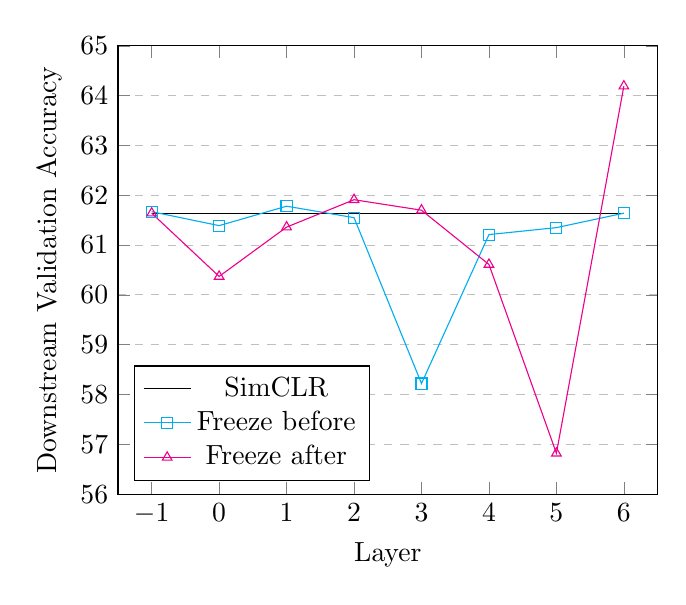
\begin{tikzpicture}
\begin{axis}[
    %title={Temperature dependence of CuSO\(_4\cdot\)5H\(_2\)O solubility},
    % width=0.8\textwidth,
    % height=0.5\textwidth,
    xlabel={Layer},
    ylabel={Downstream Validation Accuracy},
    xmin=-1.5, xmax=6.5,
    ymin=56, ymax=65,
    xtick={-1,0,1,2,3,4,5,6,7}, %,11,12,13},
    ytick={56, 57, 58, 59, 60, 61, 62, 63, 64, 65},
    %ytick={0,0.2,0.4,0.6,0.8,1.0}, %,0.6,0.7,0.8,0.9,1.0},
    legend pos=south west,
    ymajorgrids=true,
    grid style=dashed,
]
% \addplot[
%     color=black,
%     mark=diamond,
%     ]
%     coordinates {
%     % (300,62.14999771118164)(600,63.15999984741211)(900,62.91999816894531)(1200,62.29999923706055)(1500,61.93000030517578)
%     (0,61.64)
%     (1,61.64)
%     (2,61.64)
%     (3,61.64)
%     (4,61.64)
%     (5,61.64)
%     (6,61.64)
%     (7,61.64)
%     };
%     \addlegendentry{SimCLR}
\addplot[
    %dotted,
    %dashed,
    mark options={solid},
    color=black,
    %mark=diamond,
    ]
    coordinates {
    % (300,62.14999771118164)(600,63.15999984741211)(900,62.91999816894531)(1200,62.29999923706055)(1500,61.93000030517578)
    (-1,61.64)
    (0,61.64)
    (1,61.64)
    (2,61.64)
    (3,61.64)
    (4,61.64)
    (5,61.64)
    (6,61.64)
    % below is conitnue simclr
    % (-1,61.91999816894531)
    % (0,61.91999816894531)
    % (1,61.91999816894531)
    % (2,61.91999816894531)
    % (3,61.91999816894531)
    % (4,61.91999816894531)
    % (5,61.91999816894531)
    % (6,61.91999816894531)
    };
    \addlegendentry{SimCLR}
\addplot[
    color=cyan,
    mark=square,
    ]
    coordinates {
    (-1, 61.66999816894531)
    (0, 61.38999938964844)
    (1, 61.779998779296875)
    (2, 61.54999923706055)
    (3, 58.21999740600586)
    (4, 61.209999084472656)
    (5, 61.349998474121094)
    (6, 61.64)
    };
    \addlegendentry{Freeze before}
% \addplot[
%     dashed,
%     mark options={solid},
%     color=blue,
%     mark=square,
%     ]
%     coordinates {
%     (0, 61.66999816894531)
%     (1, 61.47999954223633)
%     (2, 61.939998626708984)
%     (3, 62.0099983215332)
%     (4, 62.93000030517578)
%     (5, 64.0999984741211)
%     (6, 60.09000015258789)
%     (7, 64.18999481201172)
%     };
%     \addlegendentry{Stop*}
\addplot[
    color=magenta,
    mark=triangle,
    ]
    coordinates {
    (-1, 61.64)
    (0, 60.369998931884766)
    (1, 61.3599967956543)
    (2, 61.90999984741211)
    (3, 61.69999694824219)
    (4, 60.6099967956543)
    (5, 56.81999969482422)
    (6, 64.18999481201172) % 61.91999816894531)
    };
    \addlegendentry{Freeze after}
% \addplot[
%     dashed,
%     mark options={solid},
%     color=red,
%     mark=triangle,
%     ]
%     coordinates {
%     (0, 61.66999816894531)
%     (1, 61.59000015258789)
%     (2, 61.55999755859375)
%     (3, 61.849998474121094)
%     (4, 62.21999740600586)
%     (5, 59.62999725341797)
%     (6, 58.68000030517578)
%     (7, 61.5099983215332)
%     };
%     \addlegendentry{w/o Stop*}


\end{axis}
\end{tikzpicture}
}
\vspace{-.2in}
%\caption{Continue Cifar100-Cifar100}
\caption{Freezing layers before and after Deep Augmentation with stop-gradient, initialized with pre-trained SimCLR model. For ``Freeze before," Layer -1 freezes nothing, and for ``Freeze after" Layer 6 freezes nothing.\vspace{-.2in}}
\label{fig:cifar100-cifar100-freeze}
%\vspace{-0.5cm}
\end{figure}





% \begin{figure}[ht]
% \resizebox{0.5\columnwidth}{!}{
% \centering
% \begin{tikzpicture}
% \begin{axis}[
%     %title={Temperature dependence of CuSO\(_4\cdot\)5H\(_2\)O solubility},
%     % width=0.8\textwidth,
%     % height=0.5\textwidth,
%     xlabel={Num. Epochs Pre-training},
%     ylabel={Downstream Validation Accuracy},
%     xmin=230, xmax=1540,
%     ymin=57, ymax=65,
%     xtick={200,400,600,800,1000,1200,1400}, %,11,12,13},
%     ytick={57, 58, 59, 60, 61, 62, 63, 64, 65},
%     %ytick={0,0.2,0.4,0.6,0.8,1.0}, %,0.6,0.7,0.8,0.9,1.0},
%     legend pos=south west,
%     ymajorgrids=true,
%     grid style=dashed,
% ]
% \addplot[
%     color=black,
%     mark=diamond,
%     ]
%     coordinates {
%     (300,62.79999923706055)(600,62.5)(900,62.87999725341797)(1200,62.28999710083008)(1500,61.91999816894531)
%     };
%     \addlegendentry{S}
% \addplot[
%     color=blue,
%     mark=square,
%     ]
%     coordinates {
%     (600,61.94999694824219)(900,62.209999084472656)(1200,61.939998626708984)(1500,61.66999816894531)
%     %(300,60.39999771118164)(600,61.98999786376953)(900,62.3599967956543)(1200,61.73999786376953)(1500,61.7599983215332)
%     };
%     \addlegendentry{L-1}
% \addplot[
%     color=red,
%     mark=triangle,
%     ]
%     coordinates {
%     (300,62.189998626708984)(600,62.2599983215332)(900,61.98999786376953)(1200,62.07999801635742)(1500,61.38999938964844)
%     %(300,61.03999710083008)(600,62.3599967956543)(900,62.1099967956543)(1200,62.43000030517578)(1500,61.769996643066406)
%     };
%     \addlegendentry{L0}
% \addplot[
%     color=green,
%     mark=otimes,
%     ]
%     coordinates {
%     (300,61.81999969482422)(600,62.94999694824219)(900,63.56999969482422)(1200,62.25)(1500,61.779998779296875)
%     %(300,62.28999710083008)(600,62.869998931884766)(900,63.439998626708984)(1200,63.09000015258789)(1500,62.0099983215332)
%     };
%     \addlegendentry{L1}
% \addplot[
%     color=pink,
%     mark=square,
%     ]
%     coordinates {
%     (300,61.869998931884766)(600,63.279998779296875)(900,63.69999694824219)(1200,62.03999710083008)(1500,61.54999923706055)
%     %(300,62.16999816894531)(600,62.959999084472656)(900,62.21999740600586)(1200,61.459999084472656)(1500,61.40999984741211)
%     };
%     \addlegendentry{L2}
% \addplot[
%     color=orange,
%     mark=diamond,
%     ]
%     coordinates {
%     (300,55.57999801635742)(600,55.46999740600586)(900,57.29999923706055)(1200,57.69999694824219)(1500,58.21999740600586)
%     };
%     \addlegendentry{L3}
% \addplot[
%     color=yellow,
%     mark=triangle,
%     ]
%     coordinates {
%     (300,59.97999954223633)(600,59.22999954223633)(900,60.439998626708984)(1200,60.79999923706055)(1500,61.209999084472656)
%     };
%     \addlegendentry{L4}
% \addplot[
%     color=purple,
%     mark=otimes,
%     ]
%     coordinates {
%     (300,59.30999755859375)(600,59.349998474121094)(900,59.84000015258789)(1200,60.90999984741211)(1500,61.349998474121094)
%     };
%     \addlegendentry{L5}
% % \addplot[
% %     color=teal,
% %     mark=square,
% %     ]
% %     coordinates {
% %     (300,59.599998474121094)(600,59.28999710083008)(900,60.30999755859375)(1200,60.63999938964844)(1500,61.07999801635742)
% %     % (300,59.63999938964844)(600,60.80999755859375)(900,62.57999801635742)(1200,64.29000091552734)(1500,64.18999481201172)
% %     };
% %     \addlegendentry{25}

% \end{axis}
% \end{tikzpicture}
% }
% %\vspace{-.1in}
% \caption{Freeze Continue Cifar100-Cifar100}
% \label{fig:freeze-continue-cifar100-cifar100}
% %\vspace{-0.5cm}
% \end{figure}

% \begin{figure}[ht]
% \resizebox{0.5\columnwidth}{!}{
% \centering
% \begin{tikzpicture}
% \begin{axis}[
%     %title={Temperature dependence of CuSO\(_4\cdot\)5H\(_2\)O solubility},
%     % width=0.8\textwidth,
%     % height=0.5\textwidth,
%     xlabel={Num. Epochs Pre-training},
%     ylabel={Downstream Validation Accuracy},
%     xmin=230, xmax=1540,
%     ymin=57, ymax=64,
%     xtick={200,400,600,800,1000,1200,1400}, %,11,12,13},
%     ytick={57, 58, 59, 60, 61, 62, 63, 64},
%     %ytick={0,0.2,0.4,0.6,0.8,1.0}, %,0.6,0.7,0.8,0.9,1.0},
%     legend pos=south west,
%     ymajorgrids=true,
%     grid style=dashed,
% ]
% \addplot[
%     color=black,
%     mark=diamond,
%     ]
%     coordinates {
%     (300,62.79999923706055)(600,62.5)(900,62.87999725341797)(1200,62.28999710083008)(1500,61.91999816894531)
%     };
%     \addlegendentry{S}
% % \addplot[
% %     color=blue,
% %     mark=square,
% %     ]
% %     coordinates {
% %     (600,61.94999694824219)(900,62.209999084472656)(1200,61.939998626708984)(1500,61.66999816894531)
% %     };
% %     \addlegendentry{L-1}
% \addplot[
%     color=red,
%     mark=triangle,
%     ]
%     coordinates {
%     (300,58.37999725341797)(600,58.30999755859375)(900,58.64999771118164)(1200,59.80999755859375)(1500,60.369998931884766)
%     };
%     \addlegendentry{L0}
% \addplot[
%     color=green,
%     mark=otimes,
%     ]
%     coordinates {
%     (300,59.38999938964844)(600,59.019996643066406)(900,59.8599967956543)(1200,60.28999710083008)(1500,61.3599967956543)
%     };
%     \addlegendentry{L1}
% \addplot[
%     color=pink,
%     mark=square,
%     ]
%     coordinates {
%     (300,58.68000030517578)(600,59.1099967956543)(900,60.16999816894531)(1200,61.06999969482422)(1500,61.90999984741211)
%     };
%     \addlegendentry{L2}
% \addplot[
%     color=orange,
%     mark=diamond,
%     ]
%     coordinates {
%     (300,58.519996643066406)(600,60.34000015258789)(900,59.689998626708984)(1200,61.209999084472656)(1500,61.69999694824219)
%     };
%     \addlegendentry{L3}
% \addplot[
%     color=yellow,
%     mark=triangle,
%     ]
%     coordinates {
%     (300,59.32999801635742)(600,60.05999755859375)(900,61.38999938964844)(1200,60.25)(1500,60.6099967956543)
%     };
%     \addlegendentry{L4}
% \addplot[
%     color=purple,
%     mark=otimes,
%     ]
%     coordinates {
%     (300,56.07999801635742)(600,56.53999710083008)(900,57.7599983215332)(1200,57.57999801635742)(1500,56.81999969482422)
%     };
%     \addlegendentry{L5}
% % \addplot[
% %     color=teal,
% %     mark=square,
% %     ]
% %     coordinates {
% %     (300,61.63999938964844)(600,61.97999954223633)(900,62.91999816894531)(1200,62.62999725341797)(1500,61.5099983215332)
% %     };
% %     \addlegendentry{L6}

% \end{axis}
% \end{tikzpicture}
% }
% %\vspace{-.1in}
% \caption{Continue Freeze Reverse Cifar100-Cifar100}
% \label{fig:freeze-reverse-continue-cifar100-cifar100}
% %\vspace{-0.5cm}
% \end{figure}

\subsubsection{Architecture}

% In an additional attempt to understand what makes a targeted dropout work at some layers but not others, w
Consider the layers of ResNet18 documented in Figure \ref{table:resnet18}. Layer 5 averages the convolutional filters in Layer 4; however, the performance difference between them in Figure \ref{fig:cifar100-cifar100-stop-vs-not} is considerable, while it is small for ``Freeze before" in Figure \ref{fig:cifar100-cifar100-freeze}. For Deep Augmentation, dropping information within the $4\times 4$ convolutional filters in Layer 4 is more useful than dropping complete filters. This corresponds to dropping spatial information rather than along channels (e.g.\ pixels versus colors in the input data). ``Freezing before" (Figure \ref{fig:cifar100-cifar100-freeze}) might maintain inherited spatial invariances, while not freezing (Figure \ref{fig:cifar100-cifar100-stop-vs-not}) causes the CNN to diverge from the spatial invariances, leading to reduced performance in Layer 5. 
% \justin{not sure what this means:}
%, thus explaining the difference in performance of Layer 4.
% { \color{red} 
% Perhaps for CNN architecture, dropping spatial information is more useful than along channels. In the data space, this corresponds to dropping pixels and removing a color, respectively, but it is unclear what it corresponds to higher up in the network. Initial experiment indicated that 2D-dropout (dropping complete filters) perform less well than regular dropout. Freezing (as in Figure \ref{fig:cifar100-cifar100-freeze}) could force the network to better maintain the spatial bias implicit in CNNs while training all layers (as in Figure \ref{fig:cifar100-cifar100-stop-vs-not}) could allow the NN to diverge from the spatial bias and find parameters that generalize less well, thus explaining the difference in performance of Layer 4.
% }

 

% \subsubsection{Why does it work?}

% Exploring what might affect performance, we try using the Alignment and Uniformity measures to measure the quality of an embedding space. However, these measures are defined with respect to a specific set of transformations or data augmentations. Since we make use of higher-layer transformations, it is not clear how to compare across our different experiments. We try using the SimCLR input data transformations across methods, see Figure \ref{fig:align_uniform} for results for five checkpoints (at epochs 300, 600, 900, 1200, 1500) per method. For each method, more training always lead to better (lower) Uniformity on the test data, while Alignment is always improved with more training on the Training data.


% \begin{figure}[ht]
% \resizebox{\columnwidth}{!}{%
% \begin{tikzpicture}
% \begin{axis}[
%     enlargelimits=true,
%     grid style=dashed,
%     xlabel={Uniformity},
%     ylabel={Alignment},
%     legend pos=south east,
%     % xtick={-2.77, -2.76, -2.75, -2.74, -2.73, -2.72}, %,11,12,13},
%     % ytick={1.99, 2},
% ]
% \addplot[
%     color=black,
%     only marks,
%     mark=o,
%     mark size=2.9pt]
% table[meta=Alignment]
% {data/scattered_simclr100.dat};
% \addlegendentry{SimCLR}
% \addplot[
%     color=blue,
%     only marks,
%     %scatter,
%     mark=square,
%     mark size=2.9pt]
% table[meta=Alignment]
% {data/scattered_a100l4.dat};
% \addlegendentry{L4}
% \addplot[
%     color=orange,
%     only marks,
%     %scatter,
%     mark=pentagon,
%     mark size=2.9pt]
% table[meta=Alignment]
% {data/scattered_at100l4.dat};
% \addlegendentry{TL4}
% \addplot[
%     color=red,
%     only marks,
%     %scatter,
%     mark=diamond,
%     mark size=2.9pt]
% table[meta=Alignment]
% {data/scattered_a100l5.dat};
% \addlegendentry{L5}
% \addplot[
%     color=green,
%     only marks,
%     %scatter,
%     mark=triangle,
%     mark size=2.9pt]
% table[meta=Alignment]
% {data/scattered_a100l6.dat};
% \addlegendentry{L6}
% \end{axis}
% \end{tikzpicture}
% % \caption{Alignment and Uniformity}
% % \label{fig:align_uniform}
% % \end{figure}

% % \begin{figure}[ht]
% \begin{tikzpicture}
% \begin{axis}[
%     enlargelimits=true,
%     grid style=dashed,
%     xlabel={Uniformity},
%     ylabel={Alignment},
%     legend pos=south east,
%     % xtick={-2.77, -2.76, -2.75, -2.74, -2.73, -2.72}, %,11,12,13},
%     % ytick={1.99, 2},
% ]
% \addplot[
%     color=black,
%     only marks,
%     mark=o,
%     mark size=2.9pt]
% table[meta=Alignment]
% {data_train/scattered_simclr100.dat};
% \addlegendentry{SimCLR}
% \addplot[
%     color=blue,
%     only marks,
%     %scatter,
%     mark=square,
%     mark size=2.9pt]
% table[meta=Alignment]
% {data_train/scattered_a100l4.dat};
% \addlegendentry{L4}
% \addplot[
%     color=orange,
%     only marks,
%     %scatter,
%     mark=pentagon,
%     mark size=2.9pt]
% table[meta=Alignment]
% {data_train/scattered_at100l4.dat};
% \addlegendentry{TL4}
% \addplot[
%     color=red,
%     only marks,
%     %scatter,
%     mark=diamond,
%     mark size=2.9pt]
% table[meta=Alignment]
% {data_train/scattered_a100l5.dat};
% \addlegendentry{L5}
% \addplot[
%     color=green,
%     only marks,
%     %scatter,
%     mark=triangle,
%     mark size=2.9pt]
% table[meta=Alignment]
% {data_train/scattered_a100l6.dat};
% \addlegendentry{L6}
% \end{axis}
% \end{tikzpicture}
% }
% \caption{Alignment and Uniformity (lower is better). Left: Test data. Right: Training Data}
% \label{fig:align_uniform}
% \end{figure}

% On the test set, Layer 4 and Layer 6 is beating SimCLR at its own game, i.e. it's own augmentations, achieving both better Alignmnet and Uniformity with respect to the SimCLR data augmentations. Looking at the Alignment and Uniformity on the training data, we see that Layer 4 and Layer 6 achieve better Uniformity, but that trainable Layer 4 and SimCLR achieve stronger Alignment---overfitting to the training set as Alignment on the test set increases during training. The measures of Layer 5 is worse on both training and test set, in accordance with it's downstream performance. However, even though SimCLR and trainable Layer 4 perform substantially different on the downstream task, their Alignment and Uniformity is surprisingly similar, indicating that Alignment and Uniformity does not provide a complete picture. Indeed, relying on measures dependent on the transformations or augmentations used to asses the quality of an latent space is insufficient.

% Further trying to understand why Deep Augmentation works and on what layers we use the centered kernel alignment (CKA) as a similarity index between layers across the NN. In Figure \ref{figure:barsresnet18} we include CKA for a random initialized ResNet18, after it has been trained with SimCLR, and after it has been trained with trainable Deep Augmentation after Layer 4. We include the plots for more settings in the Appendix, but most look either like SimCLR or trainable Layer 4. We note that there is a strong co-adaptation between Layer 4 and Layer 5 after they have been trained with SimCLR but not before. We also see that the poorly performing trainable Layer 4 has an even increased co-adaptation between Layer 4 and Layer 5, which is also true for poorly performing Layer 5 in the Appendix. In contrast, top performing Layer 4 and Layer 6 are very close to SimCLR. Thus, this indicates that a failure case is increased co-adaptation between layers, and that Layer 4 might be special because it is a layer after which ResNet18 is particularly susceptible to co-adaptation between itself and subsequent layers. This hints at an interpretation of Deep Augmentation as affecting co-adaptation between layers, yet it also makes sense that learning invariances to a greater granularity of augmentations leads to more specialized layers.


% \begin{figure}[ht]
% \includegraphics[width=\linewidth]{images/Bars1.png}
% \caption{Indications of why Layer 4 is special, as it is the major divide between co-adaptation across layers. All high performing NNs have the pattern of SimCLR and failure cases of T4 and Layer 5 has the pattern with stronger co-adaptation between Layer 4 and Layer 5. }
% \label{figure:barsresnet18}
% \end{figure}



% \subsection{ImageNet100 and ResNet}

% We now test the generalizability of four of our configurations to larger datasets. To accomplish this, we conducted experiments on ImageNet100 using a ResNet50 neural network, training for 1000 epochs. The results, as depicted in Figure \ref{table:imagenet100}, indicate that the overall trend is consistent across the various configurations, with Layer 6 without stop-gradient performing the best, closely followed by Layer 4 with stop-gradient. Our approach demonstrated a significant improvement over SimCLR, with an increase of nearly 3\%. This may be attributed to the small image size of the CIFAR dataset (32x32), which may result in lower quality higher-level features and reduced benefits from learning invariances with respect to them. Conversely, a more nuanced dataset with a greater variety of features may allow for greater utility in learning invariances with respect to higher-level features.

% \begin{figure}[ht]
% \centering
% \begin{tabular}{ |p{1.1cm}||p{2.2cm}|p{2.6cm}|  }
%  \hline
%  \multicolumn{3}{|c|}{ResNet50 on ImageNet100} \\
%  \hline
%  Layer & Stop-Gradient & Downstream Acc.  \\
%  \hline
%  SimCLR & N/A & 76.86\% \\
%  L4    & No        & 77.52\%  \\
%  L4     & Yes    & 79.64\%    \\
%  L5     & No    & 78.62\% \\
%  L5     & Yes    &  76.06\% \\
%  L6     & No    & 79.80\%    \\
%  L6     & Yes   & 78.62\%   \\
%  % L3     & Conv(k=3, s=2)    & 8^2\times256=16384    \\
%  % L4     & Conv(k=3, s=2)    & 4^2\times512=8192     \\
%  % L5     & Avgpool           & 512                   \\
%  % L6     & MLP               & 128                   \\
%  \hline
% \end{tabular}
% \caption{Training for a 1000 epochs on ImageNet100}
% \label{table:imagenet100}
% \end{figure}

\subsection{Sentence Embeddings and Transformer}

We experiment with Deep Augmentation applied to Transformers trained to produce sentence embeddings, using SimCSE \citep{gao-etal-2021-simcse} as a baseline.  SimCSE uses non-targeted dropout as a means of augmentation to create contrastive learning pairs.


%SimCSE employs a development set for early stopping of training that is conducted for a maximum of one epoch, finding that batch size does not significantly impact performance. 

SimCSE employs a \emph{labeled} development set, which they use to identify the best-performing model among several trained for one epoch with different hyperparameters. 
%
This labeled data is often not available in self-supervised learning.
%
Moreover, SimCSE limits training to one epoch to avoid ``forgetting'' features learned in the pre-trained BERT model, thus reducing the benefits of prolonged training. In the absence of a development set, it is essential for the training procedure to be able to generate high-quality models for a range of hyperparameters and numbers of epochs. %, as the optimal stopping point is not known a priori.

In Section \ref{sec:cifar}, we train for 1500 epochs. It was essential to employ both the SimCLR transformations and higher-layer transformations to avoid obviating the benefits of SimCLR alone. This strategy preserves the invariances from the SimCLR transformations and adds a granularity of features, from local to global,  provided by Deep Augmentation. %Invariances with respect to higher-layer invariances are global, thus it is also important to maintain the more local invariances.

For sentence embedding, SimCSE initializes with a pretrained BERT model \citep{bert}, but maintaining BERT's MLM objective in addition to SimCSE's objective severely hinders performance. The success of SimCSE may be attributed to its limited training and use of a development set, while our experiments suggest that dropout as an augmentation for sentence embeddings can be made more robust. % via Deep Augmentation.
%\justin{finish}


%, precisely adjusting the BERT latent space to new data without forgetting the pre-trained invariances from BERT's MLM objective. 

%This results in a sensitivity that is undesirable in the typical settings where a development set is not available. 


%\subsubsection{Deep Augmentation Only}

\paragraph*{Deep Augmentation Only.}
We first incorporate Deep Augmentation into the SimCSE setup without MLM; see Figure \ref{fig:simcsetop}. Layers demonstrating the best performance with stop-gradient correspond to the worst performing layers without stop-gradient, and vice versa. As in Section \ref{sec:cifar}, the stop-gradient performs better at earlier layers compared to without. We trained both with and without the 10\% attention- and hidden-dropout that BERT as well as SimCSE use and we found that their presence improves performance, results for without can be found in Appendix. In Figure \ref{fig:simcsetop}, ``Stop" and ``w/o Stop" correspond to Deep Augmentation with and without stop-gradient, respectively, optimized over dropout rates of 50\%, 25\% and 12.5\% (note that SimCSE was optimized over rates 1\%, 5\%, 10\%, 15\%, 20\%, 50\%). ``Stop*" and ``w/o Stop*" correspond to dropout rates of 50\%, which performs well and show similar trends. Several configurations outperform SimCSE and demonstrate new state-of-the-art on the STS tasks \citep{agirre-etal-2012-semeval, cer-etal-2017-semeval, marelli-etal-2014-sick}, with the best checkpoints presented in Figure \ref{table:STS}.

\begin{figure}[ht]
\centering
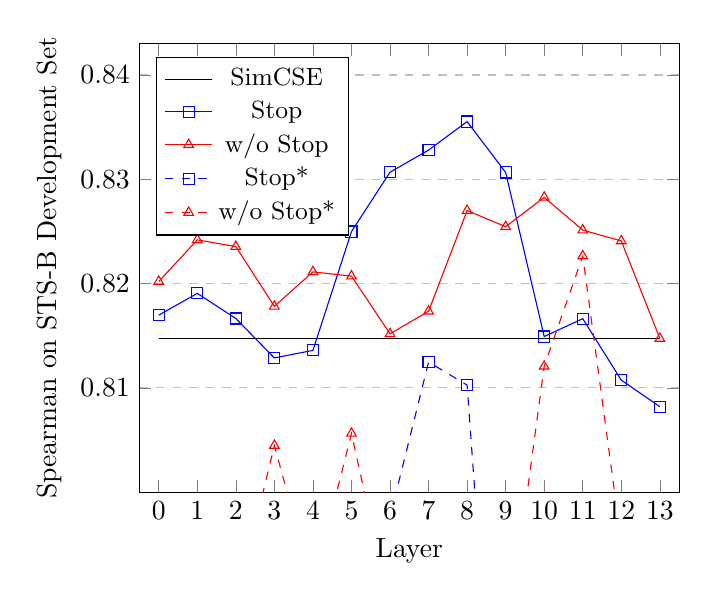
\begin{tikzpicture}
\begin{axis}[
    %title={Temperature dependence of CuSO\(_4\cdot\)5H\(_2\)O solubility},
    % width=0.8\textwidth,
    % height=0.5\textwidth,
    xlabel={Layer},
    ylabel={Spearman on STS-B Development Set},
    xmin=-0.5, xmax=13.5,
    ymin=0.8, ymax=0.843,
    xtick={0, 1, 2, 3, 4, 5, 6, 7, 8, 9, 10, 11, 12, 13}, %,11,12,13},
    ytick={0.81, 0.82, 0.83, 0.84},
    %ytick={0,0.2,0.4,0.6,0.8,1.0}, %,0.6,0.7,0.8,0.9,1.0},
    legend pos=north west,
    ymajorgrids=true,
    grid style=dashed,
]
\addplot[
    color=black,
    %mark=diamond,
    ]
    coordinates {
    (0,0.8147335170481025)(1,0.8147335170481025)(2,0.8147335170481025)(3,0.8147335170481025)(4,0.8147335170481025)(5,0.8147335170481025)(6,0.8147335170481025)(7,0.8147335170481025)(8,0.8147335170481025)(9,0.8147335170481025)(10,0.8147335170481025)(11,0.8147335170481025)(12,0.8147335170481025)(13,0.8147335170481025)
    };
    \addlegendentry{\small SimCSE}


\addplot[
    color=blue,
    mark=square,
    ]
    coordinates {
    (0,0.8169731103921712)
    (1,0.819057984441431)
    (2,0.8166468866942407)
    (3,0.812866365572481)
    (4,0.8135888411587529)
    (5,0.8249856728469834)
    (6,0.8306805778612282)
    (7,0.8328021611740035)
    (8,0.8355351495654609)
    (9,0.8306577921070178)
    (10,0.8149157851326303)
    (11,0.8166311607047543)
    (12,0.8107370794093145)
    (13,0.8081902128875393)
    };
    \addlegendentry{\small Stop}

\addplot[
    color=red,
    mark=triangle,
    ]
    coordinates {
    (0,0.8201958563827355)
    (1,0.824192633155200)
    (2,0.8235437910715707)
    (3,0.8178133056476282)
    (4,0.8211208445639191)
    (5,0.8207129410980774)
    (6,0.8151817237627103)
    (7,0.8173462234751712)
    (8,0.8270007756575324)
    (9,0.8254520877587794)
    (10,0.8282669249521344)
    (11,0.8251234611980554)
    (12,0.8240867548112837)
    (13,0.8147346771912509)
    };
    \addlegendentry{\small w/o Stop}

\addplot[
    dashed,
    mark options={solid},
    color=blue,
    mark=square,
    ]
    coordinates {
    (0,0.7632744193037913)
    (1,0.7887974973930733)
    (2,0.787675765303225)
    (3,0.7861854902547428)
    (4,0.7574942818680372)
    (5,0.7829649115225943)
    (6,0.7976033379818234)
    (7,0.8124762681613964)
    (8,0.8102590246403415)
    (9,0.7590563327667009)
    (10,0.7379011420294991)
    (11,0.6796433898476625)
    (12,0.6775176769243549)
    (13,0.691473581560862)
    };
    \addlegendentry{\small Stop*}

\addplot[
    dashed,
    mark options={solid},
    color=red,
    mark=triangle,
    ]
    coordinates {
    (0,0.7585592528117979)
    (1,0.7991558675216115)
    (2,0.7892084923382617)
    (3,0.8044671131751203)
    (4,0.7909274995641637)
    (5,0.8056261066829183)
    (6,0.7888484920901417)
    (7,0.79693944606518)
    (8,0.7913087589103663)
    (9,0.7845707685012719)
    (10,0.8120686878093089)
    (11,0.8226423410043743)
    (12,0.7952155961226167)
    (13,0.7878095073882856)
    
    };
    \addlegendentry{\small w/o Stop*}

\end{axis}
\end{tikzpicture}
\vspace{-.2in}
\caption{SimCSE vs.\ Deep Augmentation with and without stop-gradient. *: A non-tuned-dropout rate of 50\%. ``Stop": stop-gradient. Deep Augmentation outperforms SimCSE after tuning the dropout rate, and at a non-tuned 50\% dropout-rate shows similar peaks and performs on par with SimCSE, whose dropout rate was tuned extensively.\vspace{-.1in}}
\label{fig:simcsetop}
%\vspace{-0.5cm}
\end{figure}


%\subsubsection{Deep Augmentation together with MLM}
\paragraph*{Deep Augmentation together with MLM.}
We experiment with including BERT's MLM objective for all methods. By otherwise maintaining the experiment protocol of SimCSE, the results in Figure \ref{fig:simcse-mlm} were obtained. SimCSE demonstrates poor performance, even when re-optimized over dropout rates of 0\%, 1\%, 5\%, 10\%, 15\%, 20\% (``SimCSE*"). However, incorporating Deep Augmentation with an untuned 50\% dropout rate led to a significant improvement in performance. Thus, targeting a specific layer is crucial, successfully combining the invariances encouraged by MLM and the higher-layer invariances encouraged by Deep Augmentation, in a complementary manner. We believe this enables less sensitive training, less need for a development set, and the ability to train with Deep Augmentation together with MLM from scratch.

% Next we wish to explore using the MLM objective that BERT was trained with in addition to our approach, similar to what we found so useful in CIFAR and ImageNet100. Optimizing over a single epoch we find the results of \ref{fig:simcse-mlm}. SimCSE performs very badly. However, adding our targeted dropout, performance radically increases and we are approaching previous performance. By targeting a specific layer we might strike a natural balance between more local invariances encouraged by the MLM perspective as well as higher layer invariances, which allows us to use both in tandem. 

\begin{figure}[ht]
\centering
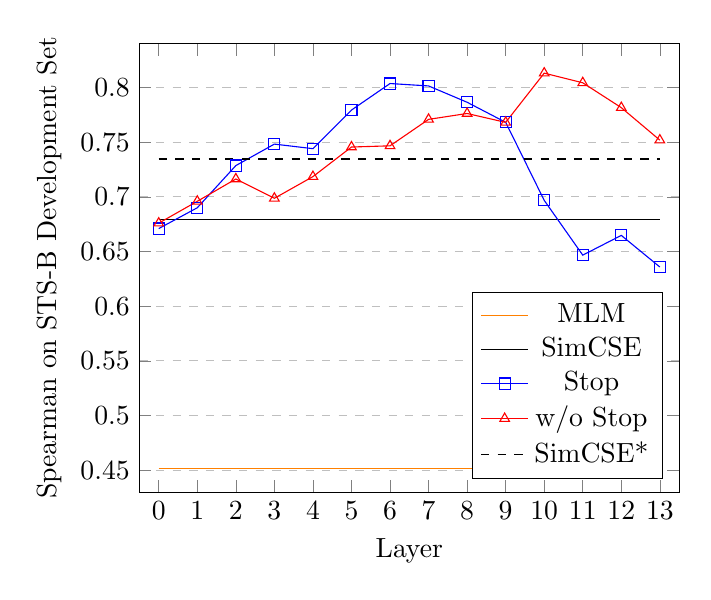
\begin{tikzpicture}
\begin{axis}[
    %title={Temperature dependence of CuSO\(_4\cdot\)5H\(_2\)O solubility},
    % width=0.8\textwidth,
    % height=0.5\textwidth,
    xlabel={Layer},
    ylabel={Spearman on STS-B Development Set},
    xmin=-0.5, xmax=13.5,
    ymin=0.43, ymax=0.84,
    xtick={0, 1, 2, 3, 4, 5, 6, 7, 8, 9, 10, 11, 12, 13}, %,11,12,13},
    ytick={0.45, 0.50, 0.55, 0.6, 0.65,0.7,0.75,0.8},
    %ytick={0,0.2,0.4,0.6,0.8,1.0}, %,0.6,0.7,0.8,0.9,1.0},
    legend pos=south east,
    ymajorgrids=true,
    grid style=dashed,
]
\addplot[
    color=orange,
    %mark=o,
    ]
    coordinates {
    (0,0.4517664038939373)(1,0.4517664038939373)(2,0.4517664038939373)(3,0.4517664038939373)(4,0.4517664038939373)(5,0.4517664038939373)(6,0.4517664038939373)(7,0.4517664038939373)(8,0.4517664038939373)(9,0.4517664038939373)(10,0.4517664038939373)(11,0.4517664038939373)(12,0.4517664038939373)(13,0.4517664038939373)
    };
    \addlegendentry{MLM}


\addplot[
    color=black,
    %mark=diamond,
    ]
    coordinates {
    (0,0.6794310092039192)(1,0.6794310092039192)(2,0.6794310092039192)(3,0.6794310092039192)(4,0.6794310092039192)(5,0.6794310092039192)(6,0.6794310092039192)(7,0.6794310092039192)(8,0.6794310092039192)(9,0.6794310092039192)(10,0.6794310092039192)(11,0.6794310092039192)(12,0.6794310092039192)(13,0.6794310092039192)
    };
    \addlegendentry{SimCSE}

\addplot[
    color=blue,
    mark=square,
    ]
    coordinates {
    (0,0.6710064393405828)
    (1,0.6900287205210686)
    (2,0.72860088650924)
    (3,0.7482461022310182)
    (4,0.744069669412655)
    (5,0.7793759991035901)
    (6,0.8036405432104125)
    (7,0.8014485968598176)
    (8,0.786510552756363)
    (9,0.7681913230485004)
    (10,0.6968147347082932)
    (11,0.6467046002123376)
    (12,0.6647613549651601)
    (13,0.6358397869890808)
    };
    \addlegendentry{Stop}

\addplot[
    color=red,
    mark=triangle,
    ]
    coordinates {
    (0,0.6759434516400763)
    (1,0.6959413906899954)
    (2,0.7163384047480618)
    (3,0.698689917495372)
    (4,0.7185099809778556)
    (5,0.7455810616864732)
    (6,0.7466678117727463)
    (7,0.7708708391301566)
    (8,0.7762493303816139)
    (9,0.7681124689016257)
    (10,0.8131356618542991)
    (11,0.8043112767687819)
    (12,0.7815920242604428)
    (13,0.7518832279573735)
    };
    \addlegendentry{w/o Stop}

\addplot[
    dashed,
    mark options={solid},
    color=black,
    %mark=diamond,
    ]
    coordinates {
    (0,0.734639170030387)
    (1,0.734639170030387)
    (2,0.734639170030387)
    (3,0.734639170030387)
    (4,0.734639170030387)
    (5,0.734639170030387)
    (6,0.734639170030387)
    (7,0.734639170030387)
    (8,0.734639170030387)
    (9,0.734639170030387)
    (10,0.734639170030387)
    (11,0.734639170030387)
    (12,0.734639170030387)
    (13,0.734639170030387)
    };
    \addlegendentry{SimCSE*}


\end{axis}
\end{tikzpicture}
\vspace{-.2in}
\caption{SimCSE vs.\ Deep Augmentation with and without stop-gradient, both with MLM. ``Stop": stop-gradient. *: includes hyperparameter search over dropout rates.\vspace{-.2in}}
\label{fig:simcse-mlm}
%\vspace{-0.5cm}
\end{figure}




\begin{figure*}[ht]
\centering
\begin{tabular}{ |p{3.2cm}||p{1.0cm}|p{1.0cm}|p{1.0cm}|p{1.0cm}|p{1.0cm}|p{1.0cm}|p{1.2cm}|p{1.0cm}|  }
 \hline
 Model & STS12 & STS13 & STS14 & STS15 & STS16 & STS-B & SICK-R & Avg. \\
 \hline
 SimCSE & 66.59 & 81.05 & 73.82 & 81.08 & \bf{79.05} & 77.55 & 71.91 & 75.86 \\
 SimCSE MLM & 49.15 & 68.76 & 54.65 & 69.64 & 72.49 & 58.02 & 63.71 & 62.35 \\
 SimCSE* MLM & 59.20 & 73.84 & 62.27 & 75.45 & 75.32 & 69.62 &  69.46 & 69.31 \\
 %Ours (S7) & 67.24 & 81.16 & 73.10 & \bf{81.48} & 78.87 & 77.29 & 70.25 & 75.63 \\
  Ours MLM (w/o Stop) & 65.25 & 80.44 & 70.65 & 79.63 & 76.75 & 76.94 & 70.58 & 74.32 \\
 Ours MLM (Stop) & 63.56 & 76.75 & 68.22 & 79.02 & 77.00 & 73.84 & 69.47 & 72.55 \\
 Ours (w/o Stop) & 68.50 & \bf{82.45} & 73.70 & 81.32 & 78.32 & 78.15 & \bf{72.12} & 76.37 \\ 
 Ours (Stop) & \bf{70.35} & 81.66 & \bf{74.11} & \bf{82.13} & 78.20 & \bf{78.59} & 72.03 &  \bf{76.72} \\
 \hline
\end{tabular}
\caption{Sentence embedding performance on STS tasks (Spearman’s correlation)}
\label{table:STS}
\end{figure*}



\section{Analysis}
\label{sec:analysis}


\subsection{Co-adaptation between Layers}
\label{sec:Co-adaptation-between-Layers}

%\subsubsection{Images and ResNet}

\paragraph*{Images and ResNet.}
%Further trying to understand why Deep Augmentation works and on what layers 
We use the centered kernel alignment (CKA) \citep{CKAsimilarity} as a similarity index between layers across a NN. Figure \ref{figure:barsresnet18} shows CKA for a random initialized ResNet18, after it has been trained with SimCLR, and after it has been trained with Deep Augmentation without stop-gradient after Layer 4. We include results for more settings in the Appendix, but most look either like ``SimCLR" or ``Layer 4 without Stop." There is strong co-adaptation between Layer 4 and 5 after training with SimCLR but not before, and poorly performing ``Layer 4 without Stop" has further increased co-adaptation between Layer 4 and 5 (which is also true for poorly performing Layer 5 in the Appendix). In contrast, top performing Layer 4 and 6 are similar to ``SimCLR." This suggests a failure case involving increased co-adaptation between layers, and that Layer 4 is special because ResNet18 is particularly susceptible to co-adaptation between Layer 4 and subsequent layers. Deep Augmentation affects co-adaptation between layers, and learning invariances to a greater granularity of augmentations should arguably lead to more specialized layers.


\begin{figure}[ht]
\includegraphics[width=\linewidth]{images/Bars1f.pdf}
\caption{Indications of why Layer 4 is special in Figure~\protect\ref{fig:cifar100-cifar100-stop-vs-not}, as it is the major divide between co-adaptation across layers. Layers 0-4 are convolutional. All high-performing NNs have the pattern of SimCLR, and failure cases have stronger co-adaptation between Layers 4 and 5. ``Layer 4 without Stop" corresponds to the failure case of Deep Augmentation without stop-gradient at Layer 4. }
\label{figure:barsresnet18}
\vspace{-.1in}
\end{figure}

%\subsubsection{Sentence Embeddings and Transformer}

\paragraph*{Sentence Embeddings and Transformer.}

\begin{figure*}[ht]
\includegraphics[width=\linewidth]{images/simcse_barsf.pdf}
\caption{CKA similarity index for ``BERT", ``SimCSE", ``Layer 10 without Stop" (Deep Augmentation without stop-gradient at Layer 10), and ``Layer 8 with Stop" (Deep Augmentation with stop-gradient at Layer 8) on STS-B. Black crosses indicate start and end of a co-adaptation region in BERT, and red crosses in ``Layer 10 without Stop" and ``Layer 8 with Stop" indicate Deep Augmentation's targets. The layers at which Deep Augmentation performs best are around the black crosses at the initialization ``BERT". CKA demonstrates the effects of Deep Augmentation as well as suggests layers to target.\vspace{-.1in}}

\label{fig:simcse_bars}
\end{figure*}

We compute the CKA similarity index for the Transformer trained under various settings, see Figure \ref{fig:simcse_bars}. ``BERT" is the starting point for both SimCSE and Deep Augmentation (``Layer 10 without Stop" and ``Layer 8 with Stop" correspond to Layer 8 with stop-gradient and Layer 10 without stop-gradient, respectively). ``BERT" has a stretch of co-adaptation between layers 8 through 11 as indicated by the two black crosses. Mirroring ResNet18 on CIFAR, it is around these two crosses that Deep Augmentation is most effective, with stop-gradient at the earlier cross and without stop-gradient at the later cross. ``SimCSE" reduces the co-adaptation across layers, especially between layers 11-10-12. In ``Layer 10 without Stop" and ``Layer 8 with Stop" the red cross indicates where Deep Augmentation was applied. ``Layer 10 without Stop" and ``Layer 8 with Stop" supersede SimCSE in their reduction of the co-adaptation among the layers following their application. 

CKA similarity index serves as a pathology and determines at what layer Deep Augmentation should be applied. Future work may investigate if simultaneously targeting multiple suitable layers further improves performance.

\subsection{Alignment and Uniformity}
\label{sec:alignment-uniformity}

% \subsubsection{Images and ResNet}
% \label{sec:alignment-uniformity-images}
\paragraph*{Images and ResNet.}

We apply the Alignment and Uniformity measures \citep{wang2020hypersphere} to assess the quality of representations. However, these measures are defined with respect to a specific set of augmentations. Since we use higher-layer transformations, it is not clear how to compare across our experiments. Thus, we use the SimCLR data transformations across methods; see Figure \ref{fig:align_uniform} for results for five checkpoints (at epochs 300, 600, 900, 1200, 1500) per method. For each method, more training leads to better (lower) Uniformity on the test data, while Alignment improves with more training on the training data.

\begin{figure}[ht]
\resizebox{\columnwidth}{!}{%
\begin{tikzpicture}
\begin{axis}[
    enlargelimits=true,
    grid style=dashed,
    xlabel={Uniformity},
    ylabel={Alignment},
    legend pos=south east,
    % xtick={-2.77, -2.76, -2.75, -2.74, -2.73, -2.72}, %,11,12,13},
    % ytick={1.99, 2},
]
\addplot[
    color=black,
    only marks,
    mark=o,
    mark size=2.9pt]
table[meta=Alignment]
{data/scattered_simclr100.dat};
\addlegendentry{SimCLR}
\addplot[
    color=blue,
    only marks,
    %scatter,
    mark=square,
    mark size=2.9pt]
table[meta=Alignment]
{data/scattered_a100l4.dat};
\addlegendentry{L4 w/ S}
\addplot[
    color=orange,
    only marks,
    %scatter,
    mark=pentagon,
    mark size=2.9pt]
table[meta=Alignment]
{data/scattered_at100l4.dat};
\addlegendentry{L4 w/o S}
\addplot[
    color=red,
    only marks,
    %scatter,
    mark=diamond,
    mark size=2.9pt]
table[meta=Alignment]
{data/scattered_a100l5.dat};
\addlegendentry{L5 w/ S}
\addplot[
    color=green,
    only marks,
    %scatter,
    mark=triangle,
    mark size=2.9pt]
table[meta=Alignment]
{data/scattered_a100l6.dat};
\addlegendentry{L6 w/ S}

\coordinate (a1) at (axis cs:-2.725,0.3);
\coordinate (a2) at (axis cs:-2.75,0.3);
\draw[->] (a1) -- (a2) node[midway,fill=white] {\emph{training}};

\end{axis}
\end{tikzpicture}
% \caption{Alignment and Uniformity}
% \label{fig:align_uniform}
% \end{figure}

% \begin{figure}[ht]
\begin{tikzpicture}
\begin{axis}[
    enlargelimits=true,
    grid style=dashed,
    xlabel={Uniformity},
    ylabel={Alignment},
    legend pos=south east,
    % xtick={-2.77, -2.76, -2.75, -2.74, -2.73, -2.72}, %,11,12,13},
    % ytick={1.99, 2},
]
\addplot[
    color=black,
    only marks,
    mark=o,
    mark size=2.9pt]
table[meta=Alignment]
{data_train/scattered_simclr100.dat};
\addlegendentry{SimCLR}
\addplot[
    color=blue,
    only marks,
    %scatter,
    mark=square,
    mark size=2.9pt]
table[meta=Alignment]
{data_train/scattered_a100l4.dat};
\addlegendentry{L4 w/ S}
\addplot[
    color=orange,
    only marks,
    %scatter,
    mark=pentagon,
    mark size=2.9pt]
table[meta=Alignment]
{data_train/scattered_at100l4.dat};
\addlegendentry{L4 w/o S}
\addplot[
    color=red,
    only marks,
    %scatter,
    mark=diamond,
    mark size=2.9pt]
table[meta=Alignment]
{data_train/scattered_a100l5.dat};
\addlegendentry{L5 w/ S}
\addplot[
    color=green,
    only marks,
    %scatter,
    mark=triangle,
    mark size=2.9pt]
table[meta=Alignment]
{data_train/scattered_a100l6.dat};
\addlegendentry{L6 w/ S}

% \draw[->] (A) -- (B) node[midway,fill=white] {\emph{success}};

\coordinate (a1) at (axis cs:-2.768,0.265);
\coordinate (a2) at (axis cs:-2.768,0.188);
\draw[->] (a1) -- (a2) node[midway,fill=white] {\emph{training}};

\end{axis}
\end{tikzpicture}
}
\vspace{-.1in}

\caption{Alignment and Uniformity (lower is better) of SimCLR augmentations on CIFAR test set. Left: Test data. Right: Training data. Deep Augmentation outperforms SimCLR when measuring alignment and uniformity \emph{using SimCLR's augmentations} on the test set, and SimCLR overfits at Alignment on the training set. ``L" is short for Layer and ``S" is short for stop-gradient. \vspace{-.1in}}
\label{fig:align_uniform}
\end{figure}

On the test set, Layer 4 and 6 (both with stop-gradient) achieve better Alignment and Uniformity with respect to the SimCLR data augmentations. The measures on the training data show that Layer 4 and 6, with stop-gradient, achieve better Uniformity. On the other hand, Layer 4 without stop-gradient and SimCLR achieves stronger Alignment---hence overfitting to the training set as Alignment on the test set worsens during training. Layer 5's measures are worse on both the training and test set, in accordance with its downstream performance. However, even though SimCLR and Layer 4 without stop-gradient perform substantially different on the downstream task, their Alignment and Uniformity are surprisingly similar, indicating that Alignment and Uniformity do not provide a complete picture. Indeed, relying on measures defined with respect to a specific augmentation, to assess the quality of a latent space is insufficient, which is why we prefer the CKA similarity index.

% \subsubsection{Sentence Embeddings and Transformer}
% \label{sec:alignment-uniformity-text}
\paragraph*{Sentence Embeddings and Transformer.}

% (which were  also used to characterize SimCSE when it was introduced)
Alignment and Uniformity measures for multiple sentence embedding methods are found in Figure \ref{fig:align_uniform_simcse}; computed in the same way as in the SimCSE work \citep{gao-etal-2021-simcse}, i.e.\ with respect to ground truth data (STS-B development set), during training, and with methods converging to higher density regions.  

\begin{figure}[ht]
\begin{tikzpicture}
\begin{axis}[
    enlargelimits=true,
    grid style=dashed,
    xlabel={Uniformity},
    ylabel={Alignment},
    % xtick={-2.77, -2.76, -2.75, -2.74, -2.73, -2.72}, %,11,12,13},
    % ytick={1.99, 2},
]

\addplot[
    color=black,
    only marks,
    mark=o,
    mark size=2.9pt
] table [x expr=\thisrowno{1},y expr=\thisrowno{0}] {data2/rep_best.txt};
\addlegendentry{SimCSE}
\addplot[
    color=blue,
    only marks,
    %scatter,
    mark=square,
    mark size=2.9pt
] table [x expr=\thisrowno{1},y expr=\thisrowno{0}] {data2/reg_best.txt};
\addlegendentry{S}
% \addplot[
%     color=blue,
%     only marks,
%     %scatter,
%     mark=square,
%     mark size=2.9pt]
% table[meta=Uniformity]
% {data2/reg_best.txt};
% \addlegendentry{L4}
\addplot[
    color=orange,
    only marks,
    %scatter,
    mark=pentagon,
    mark size=2.9pt
] table [x expr=\thisrowno{1},y expr=\thisrowno{0}] {data2/train_best.txt};
\addlegendentry{w/o S}
\addplot[
    color=red,
    only marks,
    %scatter,
    mark=triangle,
    mark size=2.9pt
] table [x expr=\thisrowno{1},y expr=\thisrowno{0}] {data2/BestREPMLM.txt};
\addlegendentry{SimCSE+MLM}
\addplot[
    color=yellow,
    only marks,
    %scatter,
    mark=o,
    mark size=2.9pt
] table [x expr=\thisrowno{1},y expr=\thisrowno{0}] {data2/REGbestMLM.txt};
\addlegendentry{S+MLM}
\addplot[
    color=green,
    only marks,
    %scatter,
    mark=triangle,
    mark size=2.9pt
] table [x expr=\thisrowno{1},y expr=\thisrowno{0}] {data2/TMLMBEST.txt};
\addlegendentry{w/o S+MLM}


% \draw[->] (A) -- (B) node[midway,fill=white] {\emph{success}};

\coordinate (o2) at (axis cs:-2.48,0.54);
\coordinate (o1) at (axis cs:-2.4,0.46);
\draw [->,orange](o1) -- (o2);
\coordinate (g1) at (axis cs:-2.40,0.44);
\coordinate (g2) at (axis cs:-2.355,0.412);
\draw [->,green](g1) -- (g2);
\coordinate (b1) at (axis cs:-2.269,0.429);
\coordinate (b2) at (axis cs:-2.333,0.47);
\draw [->,blue](b1) -- (b2);
\coordinate (s1) at (axis cs:-2.14,0.43);
\coordinate (s2) at (axis cs:-2.2,0.47);
\draw [->,black](s1) -- (s2);
\coordinate (r1) at (axis cs:-2.08,0.403);
\coordinate (r2) at (axis cs:-1.92,0.34);
\draw [->,red](r1) -- (r2);
\coordinate (y1) at (axis cs:-2.15,0.39);
\coordinate (y2) at (axis cs:-2.01,0.33);
\draw [->,yellow](y1) -- (y2);

%\draw[->,red] (3,3) -- ( $ (a)!.25!(0,0) $ ) node [midway, sloped, above] {12 m/s};

% \coordinate (a) at (3,3);
% \coordinate (b) at (3,0);
% \coordinate (c) at (-3,3);
% \node (O) at (0,0) {origin};
% \draw[->,red] (3,3) -- ( $ (a)!.25!(0,0) $ ) node [midway, sloped, above] {12 m/s};
% \draw[->,blue] (b) -- ( $ (b)!.8!(0,0) $ ) node [midway, sloped, above] {12 m/s};
% \draw[->,magenta] (c) -- ( $ (c)!.5!(0,0) $ ) node [midway, sloped, above] {12 m/s};

\end{axis}
\end{tikzpicture}
\caption{Alignment and Uniformity (lower is better) for sentence embeddings on STS-B: SimCSE vs.\ Deep Augmentation (with and without stop-gradient). We also include these methods combined with the pre-training method of BERT, i.e., Masked Language Modeling (MLM). Arrows indicate the direction during training, which  reverses when MLM is introduced. ``S" is short for stop-gradient.}
\label{fig:align_uniform_simcse}
\vspace{-.1in}
\end{figure}

Without MLM, all methods converge toward better Uniformity at the expense of Alignment. ``S" is consistently better in both measures than ``SimCSE," while ``w/o S" further encourages Uniformity at the expense of Alignment. With MLM, the direction reverses and all methods converge toward improved Alignment. Again ``S+mlm" (corresponding to MLM together with Deep Augmentation with stop-gradient) is consistently better than ``SimCSE+mlm" in both Alignment and Uniformity. On the contrary, ``w/o S+mlm" (the same but without stop-gradient) is consistently below ``S" and ``SimCSE" in both Alignment and Uniformity, but performs worse than them on downstream tasks, indicating that these measures do not paint a complete picture. %This may be due to STS-Benchmark set is a development set and thus merely a useful proxy.

\section{Discussion}

We studied higher layer transformations for enhanced self-supervised learning. Our findings demonstrate that this approach is effective when applied to both image-based contrastive learning using a ResNet architecture and sentence embedding generation using a Transformer model. We also examined the use of stop-gradient operations as well as the relationship between traditional input data transformations and higher layer transformations. Finally, we provided an interpretation of our approach as alleviating co-adaptation between layers.

% In this work we have explored the use of higher layer transformation for improved self-supervision. We show that this is useful in contrastive learning applied to images using a ResNet and to sentence embeddings using a Transformer. We explored the use of stop-gradient operation and showed that it displays distinct behavior, as well as the interactions between traditional input data transformations and the higher layer transformations. 

%%%%%%%%%%%%%%%%%%%%%%%%%
%%%%%%%%%%%%%%%%%%%%%%%%%
%%%%%%%%%%%%%%%%%%%%%%%%%
% Future research endeavors may focus on fine-tuning the hyperparameters of the proposed approach, such as determining optimal dropout rates and pairing of higher and lower transformations. It may also examine the combining of multiple targeted layers in place of a single layer.

% Another avenue would be to gain a deeper understanding of what factors contribute to the relative effectiveness of certain layers in the context of higher layer transformations, as well as explore how to design neural networks that are particularly receptive to this approach.

% Lastly, further investigation into the performance of the proposed method on larger datasets, such as the ImageNet dataset, is warranted as it holds potential for significant improvement.
%%%%%%%%%%%%%%%%%%%%%%%%%
%%%%%%%%%%%%%%%%%%%%%%%%%
%%%%%%%%%%%%%%%%%%%%%%%%%

% Future work may spend more time on tuning hyperparameters, like the dropout rate as well as at what rates to pair higher and lower transformations optimally. We should also further explore performance to bigger datasets, it looks promising to apply this approach to the full ImageNet. 

% In addition to the aforementioned areas of investigation, future work may also involve the examination of combining multiple targeted layers in place of a single layer.

%, as well as targeting layers in a sequential order. Our findings indicate that freezing early layers of a SimCLR pretrained neural network and training it with targeted transformations does improve performance. It may be worth exploring the potential benefits of iteratively moving one layer up at a time, while freezing the preceding layers, as a means of further improving performance and speed up training.

% We may also explore combining multiple targeted layers instead of a single one, as well as targeting layers in a sequential order. We found that freezing early layers of a SimCLR pretrained NN and training it with targeted transformations did improve performance. One can imagine iteratively moving one layer up at a time, freezing the preceding layers. 



% It is also interesting to better understand what makes certain layers work better than others and how one may design networks to make them extra susceptible to higher layer transformations.  

% Tune hyperparameters

% Bigger datasets

% Other networks (fix architectures so they are more appropriate for higher transformations)

% Moving up one layer at a time

% Training NN such that they're more receptible to higher transformations 

% Multiple layers targeted


{\small
\bibliographystyle{ieee_fullname}
\bibliography{egbib}
}

\clearpage
\newpage
\appendix

%%%%%%%%%%%%%%%%%%%%%%%%%%%%%%%%%%%%%%%%%%%%%%
%%%%%%%%%%%%%%%%%%%%%%%%%%%%%%%%%%%%%%%%%%%%%%
%%%%%%%%%%%%%%%%%%%%%%%%%%%%%%%%%%%%%%%%%%%%%%
%%%%%%%%%%%%%%%%%%%%%%%%%%%%%%%%%%%%%%%%%%%%%%
%%%%%%%%%%%%%%%%%%%%%%%%%%%%%%%%%%%%%%%%%%%%%%
%%%%%%%%%%%%%%%%%%%%%%%%%%%%%%%%%%%%%%%%%%%%%%
%%%%%%%%%%%%%%%%%%%%%%%%%%%%%%%%%%%%%%%%%%%%%%
%%%%%%%%%%%%%%%%%%%%%%%%%%%%%%%%%%%%%%%%%%%%%%
%%%%%%%%%%%%%%%%%%%%%%%%%%%%%%%%%%%%%%%%%%%%%%
%%%%%%%%%%%%%%%%%%%%%%%%%%%%%%%%%%%%%%%%%%%%%%
%%%%%%%%%%%%%%%%%%%%%%%%%%%%%%%%%%%%%%%%%%%%%%
%%%%%%%%%%%%%%%%%%%%%%%%%%%%%%%%%%%%%%%%%%%%%%
%%%%%%%%%%%%%%%%%%%%%%%%%%%%%%%%%%%%%%%%%%%%%%
%%%%%%%%%%%%%%%%%%%%%%%%%%%%%%%%%%%%%%%%%%%%%%
%%%%%%%%%%%%%%%%%%%%%%%%%%%%%%%%%%%%%%%%%%%%%%
%%%%%%%%%%%%%%%%%%%%%%%%%%%%%%%%%%%%%%%%%%%%%%
%%%%%%%%%      APPENDIX
%%%%%%%%%%%%%%%%%%%%%%%%%%%%%%%%%%%%%%%%%%%%%%
%%%%%%%%%%%%%%%%%%%%%%%%%%%%%%%%%%%%%%%%%%%%%%
%%%%%%%%%%%%%%%%%%%%%%%%%%%%%%%%%%%%%%%%%%%%%%
%%%%%%%%%%%%%%%%%%%%%%%%%%%%%%%%%%%%%%%%%%%%%%
%%%%%%%%%%%%%%%%%%%%%%%%%%%%%%%%%%%%%%%%%%%%%%
%%%%%%%%%%%%%%%%%%%%%%%%%%%%%%%%%%%%%%%%%%%%%%
%%%%%%%%%%%%%%%%%%%%%%%%%%%%%%%%%%%%%%%%%%%%%%
%%%%%%%%%%%%%%%%%%%%%%%%%%%%%%%%%%%%%%%%%%%%%%
%%%%%%%%%%%%%%%%%%%%%%%%%%%%%%%%%%%%%%%%%%%%%%
%%%%%%%%%%%%%%%%%%%%%%%%%%%%%%%%%%%%%%%%%%%%%%
%%%%%%%%%%%%%%%%%%%%%%%%%%%%%%%%%%%%%%%%%%%%%%
%%%%%%%%%%%%%%%%%%%%%%%%%%%%%%%%%%%%%%%%%%%%%%
%%%%%%%%%%%%%%%%%%%%%%%%%%%%%%%%%%%%%%%%%%%%%%
%%%%%%%%%%%%%%%%%%%%%%%%%%%%%%%%%%%%%%%%%%%%%%
%%%%%%%%%%%%%%%%%%%%%%%%%%%%%%%%%%%%%%%%%%%%%%
%%%%%%%%%%%%%%%%%%%%%%%%%%%%%%%%%%%%%%%%%%%%%%



\section{CIFAR}

In this section, we provide training details for our experiments on CIFAR datasets, as well as additional results and comparisons.

\subsection{Training Details}

We used the code released by \citep{supcontrast} at \href{https://github.com/HobbitLong/SupContrast}{link}. We used a batch-size of 1024 and trained each method for 1500 epochs. 

\subsection{Dropout-rates: Layer vs. Neurons}

When we specify the dropout rate for a layer, that dropout rate is only applied to that layer. Therefore, 50\% dropout at a single layer drops much fewer neurons compared to dropping 50\% of all neurons across all layers. The same dropout rate, when applied on different layers, may drop different number of neurons, as some layers have more neurons than others.

\subsection{Na\"{i}ve Deep Augmentation with stop-gradient on Cifar100}

In Figure \ref{fig:two-sided-dropout-cifar100-cifar100}, we include results of 50\% dropout with stop-gradient at individual layers on 100\% of the batch. Such na\"{i}ve augmentations generally give poor performances. All layers besides the input data layer lead to downstream accuracy of 1\% (equivalent with random guess). The input data layer arrives at a downstream accuracy of 61.38\%. 

\begin{figure}[ht]
\centering
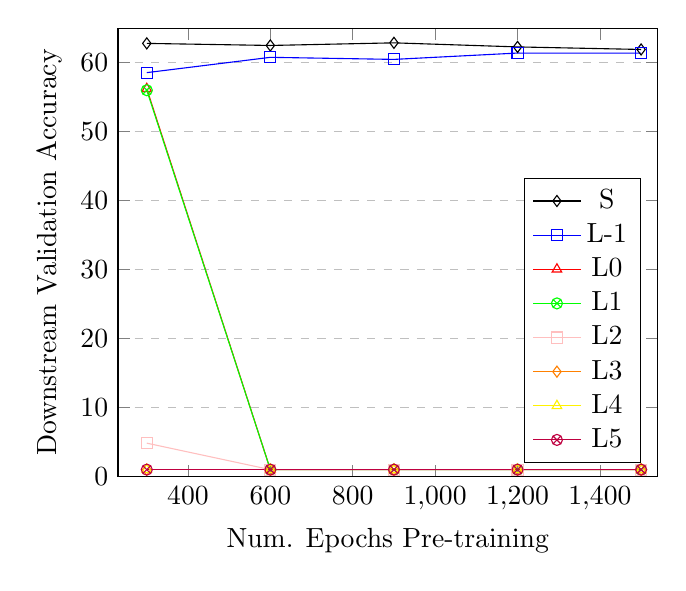
\begin{tikzpicture}
\begin{axis}[
    %title={Temperature dependence of CuSO\(_4\cdot\)5H\(_2\)O solubility},
    % width=0.8\textwidth,
    % height=0.5\textwidth,
    xlabel={Num. Epochs Pre-training},
    ylabel={Downstream Validation Accuracy},
    xmin=230, xmax=1540,
    ymin=0, ymax=65,
    xtick={200,400,600,800,1000,1200,1400}, %,11,12,13},
    ytick={0,10, 20, 30, 40, 50, 60},
    %ytick={0,0.2,0.4,0.6,0.8,1.0}, %,0.6,0.7,0.8,0.9,1.0},
    legend pos=south east,
    ymajorgrids=true,
    grid style=dashed,
]
\addplot[
    color=black,
    mark=diamond,
    ]
    coordinates {
    (300,62.79999923706055)(600,62.5)(900,62.87999725341797)(1200,62.28999710083008)(1500,61.91999816894531)
    };
    \addlegendentry{S}

\addplot[
    color=blue,
    mark=square,
    ]
    coordinates {
    (300,58.55999755859375)(600,60.779998779296875)(900,60.47999954223633)(1200,61.39999771118164)(1500,61.37999725341797)
    };
    \addlegendentry{L-1}
\addplot[
    color=red,
    mark=triangle,
    ]
    coordinates {
    (300,56.21999740600586)(600,1.0)(900,1.0)(1200,1.0)(1500,1.0)
    };
    \addlegendentry{L0}
\addplot[
    color=green,
    mark=otimes,
    ]
    coordinates {
    (300,56.0099983215332)(600,1.0)(900,1.0)(1200,1.0)(1500,1.0)
    };
    \addlegendentry{L1}
\addplot[
    color=pink,
    mark=square,
    ]
    coordinates {
    (300,4.839999675750732)(600,1.0)(900,1.0)(1200,1.0)(1500,1.0)
    };
    \addlegendentry{L2}
\addplot[
    color=orange,
    mark=diamond,
    ]
    coordinates {
    (300,1.0)(600,1.0)(900,1.0)(1200,1.0)(1500,1.0)
    };
    \addlegendentry{L3}
\addplot[
    color=yellow,
    mark=triangle,
    ]
    coordinates {
    (300,1.0)(600,1.0)(900,1.0)(1200,1.0)(1500,1.0)
    };
    \addlegendentry{L4}
\addplot[
    color=purple,
    mark=otimes,
    ]
    coordinates {
    (300,1.0)(600,1.0)(900,1.0)(1200,1.0)(1500,1.0)
    };
    \addlegendentry{L5}

\end{axis}
\end{tikzpicture}
%\vspace{-.1in}
\caption{Cifar100. 50\% dropout with stop-gradient applied at individual layers on 100\% of the batch. I.e. freezing earlier layers to random weights.}
\label{fig:two-sided-dropout-cifar100-cifar100}
%\vspace{-0.5cm}
\end{figure}

\subsection{Including Deep Augmentation w/o stop gradient initialized with SimCLR}

For completion, we also include Deep Augmentation without stop gradient, initialized with pre-trained SimCLR model, together with the other variants---see Figure \ref{fig:cifar100-cifar100-stop-vs-not-full}. We did not include it in the main part because we felt the figure got cluttered.

\begin{figure}[ht]
\centering
\resizebox{1.0\columnwidth}{!}{%
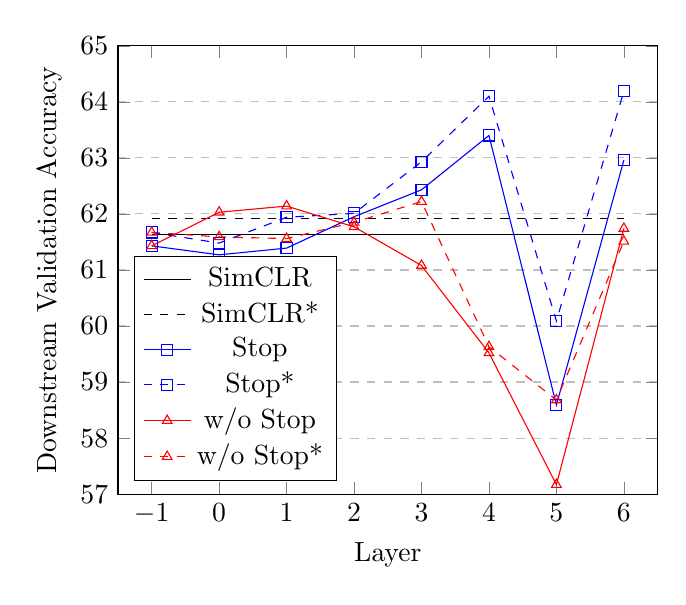
\begin{tikzpicture}
\begin{axis}[
    %title={Temperature dependence of CuSO\(_4\cdot\)5H\(_2\)O solubility},
    % width=0.8\textwidth,
    % height=0.5\textwidth,
    xlabel={Layer},
    ylabel={Downstream Validation Accuracy},
    xmin=-1.5, xmax=6.5,
    ymin=57, ymax=65,
    xtick={-1,0,1,2,3,4,5,6,7}, %,11,12,13},
    ytick={57, 58, 59, 60, 61, 62, 63, 64, 65},
    %ytick={0,0.2,0.4,0.6,0.8,1.0}, %,0.6,0.7,0.8,0.9,1.0},
    legend pos=south west,
    ymajorgrids=true,
    grid style=dashed,
]
\addplot[
    color=black,
    %mark=diamond,
    ]
    coordinates {
    % (300,62.14999771118164)(600,63.15999984741211)(900,62.91999816894531)(1200,62.29999923706055)(1500,61.93000030517578)
    (-1,61.64)
    (0,61.64)
    (1,61.64)
    (2,61.64)
    (3,61.64)
    (4,61.64)
    (5,61.64)
    (6,61.64)
    };
    \addlegendentry{SimCLR}
\addplot[
    %dotted,
    dashed,
    mark options={solid},
    color=black,
    %mark=diamond,
    ]
    coordinates {
    % (300,62.14999771118164)(600,63.15999984741211)(900,62.91999816894531)(1200,62.29999923706055)(1500,61.93000030517578)
    (-1,61.91999816894531)
    (0,61.91999816894531)
    (1,61.91999816894531)
    (2,61.91999816894531)
    (3,61.91999816894531)
    (4,61.91999816894531)
    (5,61.91999816894531)
    (6,61.91999816894531)
    };
    \addlegendentry{SimCLR*}
\addplot[
    color=blue,
    mark=square,
    ]
    coordinates {
    (-1, 61.43000030517578)
    (0, 61.269996643066406) 
    (1, 61.38999938964844)
    (2, 61.94999694824219)
    (3, 62.43000030517578)
    (4, 63.39999771118164)
    (5, 58.59000015258789)
    (6, 62.959999084472656)
    };
    \addlegendentry{Stop}
\addplot[
    dashed,
    mark options={solid},
    color=blue,
    mark=square,
    ]
    coordinates {
    (-1, 61.66999816894531)
    (0, 61.47999954223633)
    (1, 61.939998626708984)
    (2, 62.0099983215332)
    (3, 62.93000030517578)
    (4, 64.0999984741211)
    (5, 60.09000015258789)
    (6, 64.18999481201172)
    };
    \addlegendentry{Stop*}
\addplot[
    color=red,
    mark=triangle,
    ]
    coordinates {
    (-1, 61.43000030517578)
    (0, 62.029998779296875)
    (1, 62.13999938964844)
    (2, 61.769996643066406)
    (3, 61.07999801635742)
    (4, 59.519996643066406)
    (5, 57.16999816894531)
    (6, 61.73999786376953)
    };
    \addlegendentry{w/o Stop}
\addplot[
    dashed,
    mark options={solid},
    color=red,
    mark=triangle,
    ]
    coordinates {
    (-1, 61.66999816894531)
    (0, 61.59000015258789)
    (1, 61.55999755859375)
    (2, 61.849998474121094)
    (3, 62.21999740600586)
    (4, 59.62999725341797)
    (5, 58.68000030517578)
    (6, 61.5099983215332)
    };
    \addlegendentry{w/o Stop*}


\end{axis}
\end{tikzpicture}
}
%\vspace{-.1in}
%\caption{Continue Cifar100-Cifar100}
\caption{Comparing sampling 50\% and applying 50\% dropout, with or without stop-gradient. *: initialized with pre-trained SimCLR model. Stop: short for stop-gradient.}
\label{fig:cifar100-cifar100-stop-vs-not-full}
%\vspace{-0.5cm}
\end{figure}

\subsection{Domain-transfer: Cifar100 to Cifar10}
%\subsection{Cifar100 to Cifar10 domain transfer}

We perform basic domain-transfer experiments by taking networks pretrained on Cifar100 and finetuning them on Cifar10. In Figure \ref{fig:cifar100-cifar10-domain-transfer} we include results comparing SimCLR with Deep Augmentation with and without stop-gradient, across layers. We also include performance for different checkpoints across training, see Figure \ref{fig:cifar100-cifar10-stop} and Figure \ref{fig:cifar100-cifar10-train} for Deep Augmentation with and without stop gradient, respectively. Note the overfitting tendencies.

\begin{figure}[ht]
\centering
\resizebox{1.0\columnwidth}{!}{%
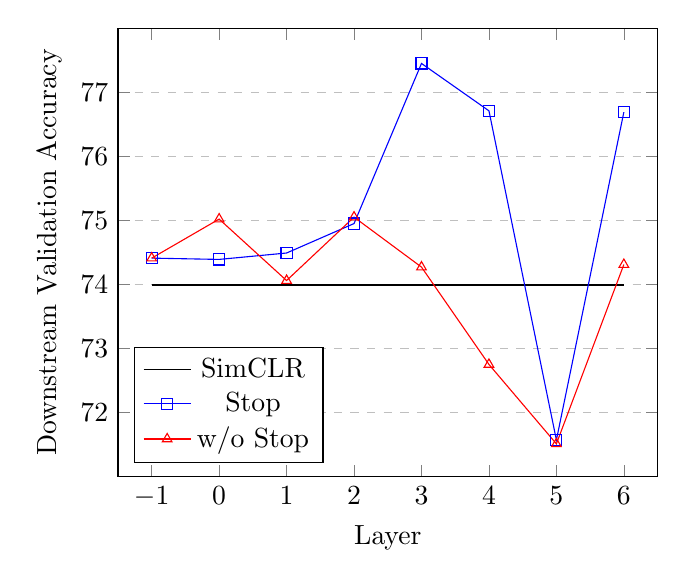
\begin{tikzpicture}
\begin{axis}[
    %title={Temperature dependence of CuSO\(_4\cdot\)5H\(_2\)O solubility},
    % width=0.8\textwidth,
    % height=0.5\textwidth,
    xlabel={Layer},
    ylabel={Downstream Validation Accuracy},
    xmin=-1.5, xmax=6.5,
    ymin=71, ymax=78,
    xtick={-1,0,1,2,3,4,5,6,7}, %,11,12,13},
    ytick={72,73,74,75,76,77},
    %ytick={0,0.2,0.4,0.6,0.8,1.0}, %,0.6,0.7,0.8,0.9,1.0},
    legend pos=south west,
    ymajorgrids=true,
    grid style=dashed,
]
\addplot[
    color=black,
    %mark=diamond,
    ]
    coordinates {
    % (300,62.14999771118164)(600,63.15999984741211)(900,62.91999816894531)(1200,62.29999923706055)(1500,61.93000030517578)
    (-1,73.98999786376953)
    (0,73.98999786376953)
    (1,73.98999786376953)
    (2,73.98999786376953)
    (3,73.98999786376953)
    (4,73.98999786376953)
    (5,73.98999786376953)
    (6,73.98999786376953)
    };
    \addlegendentry{SimCLR}
% \addplot[
%     %dotted,
%     dashed,
%     mark options={solid},
%     color=black,
%     mark=diamond,
%     ]
%     coordinates {
%     % (300,62.14999771118164)(600,63.15999984741211)(900,62.91999816894531)(1200,62.29999923706055)(1500,61.93000030517578)
%     (-1,61.91999816894531)
%     (0,61.91999816894531)
%     (1,61.91999816894531)
%     (2,61.91999816894531)
%     (3,61.91999816894531)
%     (4,61.91999816894531)
%     (5,61.91999816894531)
%     (6,61.91999816894531)
%     };
%     \addlegendentry{S}
\addplot[
    color=blue,
    mark=square,
    ]
    coordinates {
    (-1, 74.40999603271484)
    (0, 74.38999938964844)
    (1, 74.48999786376953)
    (2, 74.94999694824219)
    (3, 77.45)
    (4, 76.70999908447266)
    (5, 71.56999969482422)
    (6, 76.68999481201172)
    };
    \addlegendentry{Stop}
% \addplot[
%     dashed,
%     mark options={solid},
%     color=blue,
%     mark=square,
%     ]
%     coordinates {
%     (-1, 61.66999816894531)
%     (0, 61.47999954223633)
%     (1, 61.939998626708984)
%     (2, 62.0099983215332)
%     (3, 62.93000030517578)
%     (4, 64.0999984741211)
%     (5, 60.09000015258789)
%     (6, 64.18999481201172)
%     };
%     \addlegendentry{Stop*}
\addplot[
    color=red,
    mark=triangle,
    ]
    coordinates {
    (-1, 74.40999603271484)
    (0, 75.0199966430664)
    (1, 74.05999755859375)
    (2, 75.04999542236328)
    (3, 74.2699966430664)
    (4, 72.75)
    (5, 71.50999450683594)
    (6, 74.30999755859375)
    };
    \addlegendentry{w/o Stop}
% \addplot[
%     dashed,
%     mark options={solid},
%     color=red,
%     mark=triangle,
%     ]
%     coordinates {
%     (0, 61.66999816894531)
%     (1, 61.59000015258789)
%     (2, 61.55999755859375)
%     (3, 61.849998474121094)
%     (4, 62.21999740600586)
%     (5, 59.62999725341797)
%     (6, 58.68000030517578)
%     (7, 61.5099983215332)
%     };
%     \addlegendentry{w/o Stop*}


\end{axis}
\end{tikzpicture}
}
%\vspace{-.1in}
%\caption{Continue Cifar100-Cifar100}
\caption{Finetuning on Cifar10 of networks pre-trained on Cifar100. Comparing SimCLR with Deep Augmentation with and without stop-gradient. Stop: short for stop-gradient.}
\label{fig:cifar100-cifar10-domain-transfer}
%\vspace{-0.5cm}
\end{figure}

% \begin{figure}[ht]
% \centering
% \begin{tikzpicture}
% \begin{axis}[
%     %title={Temperature dependence of CuSO\(_4\cdot\)5H\(_2\)O solubility},
%     % width=0.8\textwidth,
%     % height=0.5\textwidth,
%     xlabel={Num. Epochs},
%     ylabel={Downstream Validation Accuracy},
%     xmin=230, xmax=1540,
%     ymin=74, ymax=80,
%     xtick={200,400,600,800,1000,1200,1400}, %,11,12,13},
%     ytick={75,76,77,78,79,80},
%     %ytick={0,0.2,0.4,0.6,0.8,1.0}, %,0.6,0.7,0.8,0.9,1.0},
%     legend pos=south west,
%     ymajorgrids=true,
%     grid style=dashed,
% ]
% \addplot[
%     color=black,
%     mark=diamond,
%     ]
%     coordinates {
%     (300,77.36000061035156)(600,77.79000091552734)(900,76.87999725341797)(1200,75.47000122070312)(1500,73.98999786376953)
%     };
%     \addlegendentry{S}

% \addplot[
%     color=blue,
%     mark=square,
%     ]
%     coordinates {
%     (600,76.98999786376953)(900,76.72000122070312)(1200,75.50999450683594)(1500,74.40999603271484)
%     };
%     \addlegendentry{L-1}
    
% \addplot[
%     color=red,
%     mark=triangle,
%     ]
%     coordinates {
%     (600,77.22000122070312)(900,76.94999694824219)(1200,74.88999938964844)(1500,74.38999938964844)
%     };
%     \addlegendentry{L0}
% \addplot[
%     color=green,
%     mark=otimes,
%     ]
%     coordinates {
%     (600,77.61000061035156)(900,77.25999450683594)(1200,75.38999938964844)(1500,74.48999786376953)
%     };
%     \addlegendentry{L1}
    
% \addplot[
%     color=pink,
%     mark=square,
%     ]
%     coordinates {
%     (600,77.83000183105469)(900,76.04999542236328)(1200,75.79000091552734)(1500,74.94999694824219)
%     };
%     \addlegendentry{L2}
% \addplot[
%     color=orange,
%     mark=diamond,
%     ]
%     coordinates {
%     (600,76.37999725341797)(900,76.75)(1200,76.93000030517578)(1500,77.45)
%     };
%     \addlegendentry{L3}
% \addplot[
%     color=yellow,
%     mark=triangle,
%     ]
%     coordinates {
%     (600,78.0199966430664)(900,79.18999481201172)(1200,78.1500015258789)(1500,76.70999908447266)
%     };
%     \addlegendentry{L4}
% \addplot[
%     color=purple,
%     mark=otimes,
%     ]
%     coordinates {
%     (600,75.16999816894531)(900,74.86000061035156)(1200,73.45999908447266)(1500,71.56999969482422)
%     };
%     \addlegendentry{L5}
% \addplot[
%     color=teal,
%     mark=square,
%     ]
%     coordinates {
%     (600,76.52999877929688)(900,78.55999755859375)(1200,78.0999984741211)(1500,76.68999481201172)
%     };
%     \addlegendentry{L6}

% \end{axis}
% \end{tikzpicture}
% %\vspace{-.1in}
% \caption{SimCLR and Deep Augmenation with stop-gradient pre-trained on Cifar100 and finetuned on Cifar10, for different checkpoint during training. Observe the overfitting behavior.}
% \label{fig:cifar100-cifar10-stop}
% %\vspace{-0.5cm}
% \end{figure}

% \begin{figure}[ht]
% \centering
% \begin{tikzpicture}
% \begin{axis}[
%     %title={Temperature dependence of CuSO\(_4\cdot\)5H\(_2\)O solubility},
%     % width=0.8\textwidth,
%     % height=0.5\textwidth,
%     xlabel={Num. Epochs},
%     ylabel={Downstream Validation Accuracy},
%     xmin=230, xmax=1540,
%     ymin=74, ymax=80,
%     xtick={200,400,600,800,1000,1200,1400}, %,11,12,13},
%     ytick={75,76,77,78,79,80},
%     %ytick={0,0.2,0.4,0.6,0.8,1.0}, %,0.6,0.7,0.8,0.9,1.0},
%     legend pos=south west,
%     ymajorgrids=true,
%     grid style=dashed,
% ]
% \addplot[
%     color=black,
%     mark=diamond,
%     ]
%     coordinates {
%     (300,77.36000061035156)(600,77.79000091552734)(900,76.87999725341797)(1200,75.47000122070312)(1500,73.98999786376953)
%     };
%     \addlegendentry{S}
% \addplot[
%     color=blue,
%     mark=square,
%     ]
%     coordinates {
%     (600,76.98999786376953)(900,76.72000122070312)(1200,75.50999450683594)(1500,74.40999603271484)
%     };
%     \addlegendentry{L-1}
% \addplot[
%     color=red,
%     mark=triangle,
%     ]
%     coordinates {
%     (600,77.88999938964844)(900,77.16999816894531)(1200,76.0199966430664)(1500,75.0199966430664)
%     };
%     \addlegendentry{L0}
% \addplot[
%     color=green,
%     mark=otimes,
%     ]
%     coordinates {
%     (600,77.9000015258789)(900,76.87999725341797)(1200,75.62999725341797)(1500,74.05999755859375)
%     };
%     \addlegendentry{L1}
    
% \addplot[
%     color=pink,
%     mark=square,
%     ]
%     coordinates {
%     (600,77.72000122070312)(900,77.2699966430664)(1200,75.72000122070312)(1500,75.04999542236328)
%     };
%     \addlegendentry{L2}
% \addplot[
%     color=orange,
%     mark=diamond,
%     ]
%     coordinates {
%     (600,77.83000183105469)(900,76.44999694824219)(1200,76.15999603271484)(1500,74.2699966430664)
%     };
%     \addlegendentry{L3}
% \addplot[
%     color=yellow,
%     mark=triangle,
%     ]
%     coordinates {
%     (600,75.0999984741211)(900,74.9000015258789)(1200,74.38999938964844)(1500,72.75)
%     };
%     \addlegendentry{L4}
% \addplot[
%     color=purple,
%     mark=otimes,
%     ]
%     coordinates {
%     (600,74.6500015258789)(900,73.94999694824219)(1200,72.54999542236328)(1500,71.50999450683594)
%     };
    
%     \addlegendentry{L5}
% \addplot[
%     color=teal,
%     mark=square,
%     ]
%     coordinates {
%     (600,78.22999572753906)(900,77.80999755859375)(1200,76.73999786376953)(1500,74.30999755859375)
%     };
%     \addlegendentry{L6}

% \end{axis}
% \end{tikzpicture}
% %\vspace{-.1in}
% \caption{SimCLR and Deep Augmenation without stop-gradient pre-trained on Cifar100 and finetuned on Cifar10, for different checkpoint during training. Observe the overfitting behavior.}
% \label{fig:cifar100-cifar10-train}
% %\vspace{-0.5cm}
% \end{figure}


\begin{figure}
\begin{subfigure}{.49\columnwidth}
\resizebox{\columnwidth}{!}{%
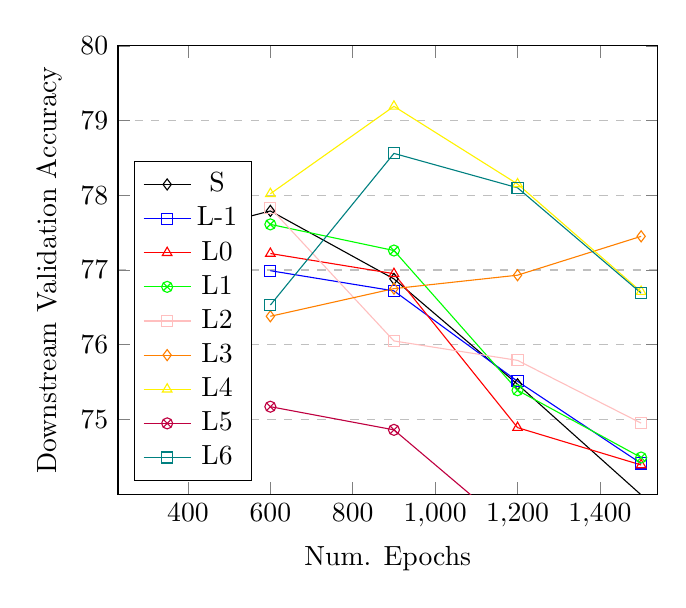
\begin{tikzpicture}
\begin{axis}[
    %title={Temperature dependence of CuSO\(_4\cdot\)5H\(_2\)O solubility},
    % width=0.8\textwidth,
    % height=0.5\textwidth,
    xlabel={Num. Epochs},
    ylabel={Downstream Validation Accuracy},
    xmin=230, xmax=1540,
    ymin=74, ymax=80,
    xtick={200,400,600,800,1000,1200,1400}, %,11,12,13},
    ytick={75,76,77,78,79,80},
    %ytick={0,0.2,0.4,0.6,0.8,1.0}, %,0.6,0.7,0.8,0.9,1.0},
    legend pos=south west,
    ymajorgrids=true,
    grid style=dashed,
]
\addplot[
    color=black,
    mark=diamond,
    ]
    coordinates {
    (300,77.36000061035156)(600,77.79000091552734)(900,76.87999725341797)(1200,75.47000122070312)(1500,73.98999786376953)
    };
    \addlegendentry{S}

\addplot[
    color=blue,
    mark=square,
    ]
    coordinates {
    (600,76.98999786376953)(900,76.72000122070312)(1200,75.50999450683594)(1500,74.40999603271484)
    };
    \addlegendentry{L-1}
    
\addplot[
    color=red,
    mark=triangle,
    ]
    coordinates {
    (600,77.22000122070312)(900,76.94999694824219)(1200,74.88999938964844)(1500,74.38999938964844)
    };
    \addlegendentry{L0}
\addplot[
    color=green,
    mark=otimes,
    ]
    coordinates {
    (600,77.61000061035156)(900,77.25999450683594)(1200,75.38999938964844)(1500,74.48999786376953)
    };
    \addlegendentry{L1}
    
\addplot[
    color=pink,
    mark=square,
    ]
    coordinates {
    (600,77.83000183105469)(900,76.04999542236328)(1200,75.79000091552734)(1500,74.94999694824219)
    };
    \addlegendentry{L2}
\addplot[
    color=orange,
    mark=diamond,
    ]
    coordinates {
    (600,76.37999725341797)(900,76.75)(1200,76.93000030517578)(1500,77.45)
    };
    \addlegendentry{L3}
\addplot[
    color=yellow,
    mark=triangle,
    ]
    coordinates {
    (600,78.0199966430664)(900,79.18999481201172)(1200,78.1500015258789)(1500,76.70999908447266)
    };
    \addlegendentry{L4}
\addplot[
    color=purple,
    mark=otimes,
    ]
    coordinates {
    (600,75.16999816894531)(900,74.86000061035156)(1200,73.45999908447266)(1500,71.56999969482422)
    };
    \addlegendentry{L5}
\addplot[
    color=teal,
    mark=square,
    ]
    coordinates {
    (600,76.52999877929688)(900,78.55999755859375)(1200,78.0999984741211)(1500,76.68999481201172)
    };
    \addlegendentry{L6}
    
\end{axis}
\end{tikzpicture}
%\vspace{-.1in}

}
%\vspace{-.1in}
\caption{With stop-gradient.}
\label{fig:cifar100-cifar10-stop}
\end{subfigure}%
\hspace{0.005\columnwidth}
\begin{subfigure}{.49\columnwidth}
\centering
\resizebox{\columnwidth}{!}{%
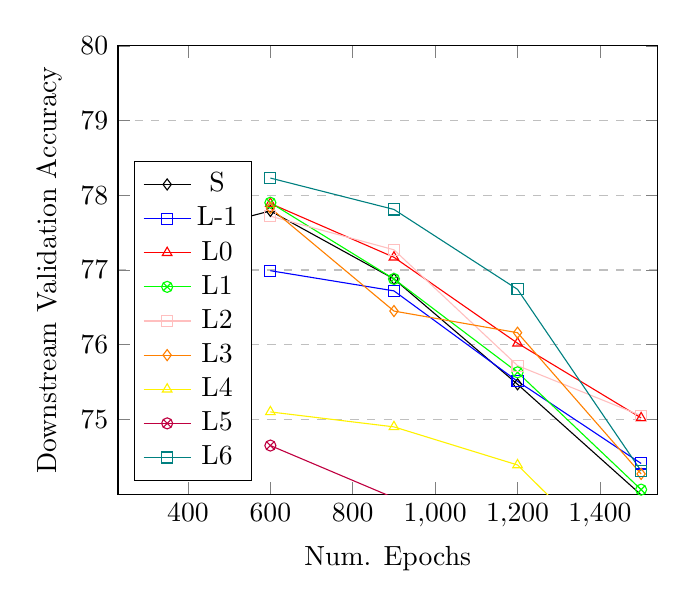
\begin{tikzpicture}
\begin{axis}[
    %title={Temperature dependence of CuSO\(_4\cdot\)5H\(_2\)O solubility},
    % width=0.8\textwidth,
    % height=0.5\textwidth,
    xlabel={Num. Epochs},
    ylabel={Downstream Validation Accuracy},
    xmin=230, xmax=1540,
    ymin=74, ymax=80,
    xtick={200,400,600,800,1000,1200,1400}, %,11,12,13},
    ytick={75,76,77,78,79,80},
    %ytick={0,0.2,0.4,0.6,0.8,1.0}, %,0.6,0.7,0.8,0.9,1.0},
    legend pos=south west,
    ymajorgrids=true,
    grid style=dashed,
]
\addplot[
    color=black,
    mark=diamond,
    ]
    coordinates {
    (300,77.36000061035156)(600,77.79000091552734)(900,76.87999725341797)(1200,75.47000122070312)(1500,73.98999786376953)
    };
    \addlegendentry{S}
\addplot[
    color=blue,
    mark=square,
    ]
    coordinates {
    (600,76.98999786376953)(900,76.72000122070312)(1200,75.50999450683594)(1500,74.40999603271484)
    };
    \addlegendentry{L-1}
\addplot[
    color=red,
    mark=triangle,
    ]
    coordinates {
    (600,77.88999938964844)(900,77.16999816894531)(1200,76.0199966430664)(1500,75.0199966430664)
    };
    \addlegendentry{L0}
\addplot[
    color=green,
    mark=otimes,
    ]
    coordinates {
    (600,77.9000015258789)(900,76.87999725341797)(1200,75.62999725341797)(1500,74.05999755859375)
    };
    \addlegendentry{L1}
    
\addplot[
    color=pink,
    mark=square,
    ]
    coordinates {
    (600,77.72000122070312)(900,77.2699966430664)(1200,75.72000122070312)(1500,75.04999542236328)
    };
    \addlegendentry{L2}
\addplot[
    color=orange,
    mark=diamond,
    ]
    coordinates {
    (600,77.83000183105469)(900,76.44999694824219)(1200,76.15999603271484)(1500,74.2699966430664)
    };
    \addlegendentry{L3}
\addplot[
    color=yellow,
    mark=triangle,
    ]
    coordinates {
    (600,75.0999984741211)(900,74.9000015258789)(1200,74.38999938964844)(1500,72.75)
    };
    \addlegendentry{L4}
\addplot[
    color=purple,
    mark=otimes,
    ]
    coordinates {
    (600,74.6500015258789)(900,73.94999694824219)(1200,72.54999542236328)(1500,71.50999450683594)
    };
    
    \addlegendentry{L5}
\addplot[
    color=teal,
    mark=square,
    ]
    coordinates {
    (600,78.22999572753906)(900,77.80999755859375)(1200,76.73999786376953)(1500,74.30999755859375)
    };
    \addlegendentry{L6}

\end{axis}
\end{tikzpicture}


}
\caption{Without stop-gradient}
\label{fig:cifar100-cifar10-train}
\end{subfigure}
\caption{SimCLR and Deep Augmenation with and without stop-gradient pre-trained on Cifar100 and finetuned on Cifar10, for different checkpoints during training. Observe the overfitting behavior.}
\label{fig:cifar100-cifar10}
\end{figure}

\subsection{Cifar10}

We include results on most of the experiments that were run on Cifar100, also on Cifar10. In general, results show the same trends as for Cifar100. In Figure \ref{fig:cifar10-cifar10-drop-all-vs-layer}, we include results comparing dropout rates across all layers to 50\% dropout at single layers. Again, we see targeted dropout at some layers showing much better performance than dropout across all layers. 

In Figure \ref{fig:cifar10-compare} we include results of sampling 50\% of batch and performing 50\% dropout with and without stop-gradient, called ``Stop" and ``w/o Stop" respectively. We also include a benchmark of SimCLR. Here ``*" refers to the networks being initialized by a pre-trained SimCLR model. Again, we see Layer 4 (with stop-gradient) and Layer 6 (with and without stop-gradient) stand out. It is also interesting to note that when initializing with a pre-trained SimCLR model, performance differs significantly more for Deep Augmentation with stop-gradient than without.

In Figure \ref{fig:cifar10-freeze}, we include results of Deep Augmentation with stop-gradient but freezing layers up to the targeted layer versus freezing after the targeted layer. Again, we see the performance change, especially Layer 3 and 4 degrading, while Layer 2 improves. 

We perform basic domain-transfer experiments by taking networks pretrained on Cifar10 and finetuning them on Cifar100. In Figure \ref{fig:cifar10-cifar100-domain} we include results comparing SimCLR with Deep Augmentation with and without stop-gradient, across layers. We also include performance for different checkpoints across training, see Figure \ref{fig:cifar10-cifar100-stop} and Figure \ref{fig:cifar10-cifar100-train} for Deep Augmentation with and without stop gradient, respectively. Note the overfitting tendencies.

\begin{figure}[ht]
\centering
\resizebox{1.0\columnwidth}{!}{%
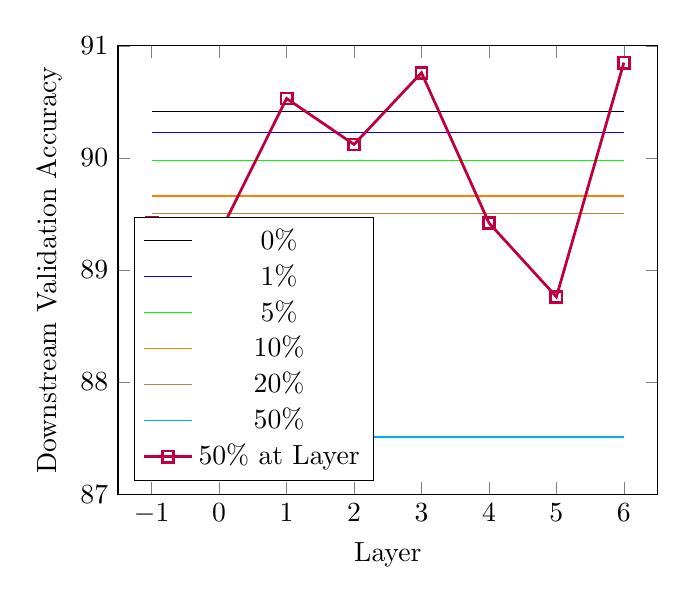
\begin{tikzpicture}
\begin{axis}[
    %title={Temperature dependence of CuSO\(_4\cdot\)5H\(_2\)O solubility},
    % width=0.8\textwidth,
    % height=0.5\textwidth,
    xlabel={Layer},
    ylabel={Downstream Validation Accuracy},
    xmin=-1.5, xmax=6.5,
    ymin=87, ymax=91,
    xtick={-1,0,1,2,3,4,5,6,7}, %,11,12,13},
    %ytick={51,52,53,54,55,56,57,58,59,60,61,62,63,64,65},
    ytick={87,88,89,90,91}, % ,52,53,54,55,56,57,58,59,60,61,62,63,64,65},
    %ytick={0,0.2,0.4,0.6,0.8,1.0}, %,0.6,0.7,0.8,0.9,1.0},
    legend pos=south west,
    %ymajorgrids=true,
    %grid style=dashed,
]
\addplot[
    %dashed,
    mark options={solid},
    color=black,
    %mark=diamond,
    ]
    coordinates {
    % (300,62.14999771118164)(600,63.15999984741211)(900,62.91999816894531)(1200,62.29999923706055)(1500,61.93000030517578)
    (-1,90.40999603271484)
    (0,90.40999603271484)
    (1,90.40999603271484)
    (2,90.40999603271484)
    (3,90.40999603271484)
    (4,90.40999603271484)
    (5,90.40999603271484)
    (6,90.40999603271484)
    };
    \addlegendentry{0\%}
\addplot[
    %dashed,
    mark options={solid},
    color=blue,
    %mark=pentagon,
    ]
    coordinates {
    (-1, 90.22999572753906)
    (0, 90.22999572753906) 
    (1, 90.22999572753906)
    (2, 90.22999572753906)
    (3, 90.22999572753906)
    (4, 90.22999572753906)
    (5, 90.22999572753906)
    (6, 90.22999572753906)
    };
    \addlegendentry{1\%}
\addplot[
    %dashed,
    mark options={solid},
    color=green,
    %mark=triangle,
    ]
    coordinates {
    (-1, 89.97999572753906)
    (0, 89.97999572753906)
    (1, 89.97999572753906)
    (2, 89.97999572753906)
    (3, 89.97999572753906)
    (4, 89.97999572753906)
    (5, 89.97999572753906)
    (6, 89.97999572753906)
    };
    \addlegendentry{5\%}
\addplot[
    %dashed,
    mark options={solid},
    color=orange,
    %mark=o,
    ]
    coordinates {
    (-1, 89.65999603271484)
    (0, 89.65999603271484)
    (1, 89.65999603271484)
    (2, 89.65999603271484)
    (3, 89.65999603271484)
    (4, 89.65999603271484)
    (5, 89.65999603271484)
    (6, 89.65999603271484)
    };
    \addlegendentry{10\%}
\addplot[
    %dashed,
    mark options={solid},
    color=brown,
    %mark=diamond,
    ]
    coordinates {
    (-1, 89.5)
    (0, 89.5)
    (1, 89.5)
    (2, 89.5)
    (3, 89.5)
    (4, 89.5)
    (5, 89.5)
    (6, 89.5)
    };
    \addlegendentry{20\%}
\addplot[
    %dashed,
    mark options={solid},
    color=cyan,
    %mark=square,
    ]
    coordinates {
    (-1, 87.50999450683594)
    (0, 87.50999450683594)
    (1, 87.50999450683594)
    (2, 87.50999450683594)
    (3, 87.50999450683594)
    (4, 87.50999450683594)
    (5, 87.50999450683594)
    (6, 87.50999450683594)
    };
    \addlegendentry{50\%}

\addplot[
    % dashed,
    % mark options={solid},
    %very thick,
    line width=1pt,
    color=purple,
    mark=square,
    ]
    coordinates {
    (-1, 89.41999816894531)
    (0, 89.31999969482422)
    (1, 90.52999877929688)
    (2, 90.1199951171875)
    (3, 90.75999450683594)
    (4, 89.41999816894531)
    (5, 88.75999450683594)
    (6, 90.8499984741211)
    % (-1, 90.3699951171875)
    % (0, 90.41999816894531)
    % (1, 90.54000091552734)
    % (2, 90.40999603271484)
    % (3, 90.40999603271484)
    % (4, 89.80999755859375)
    % (5, 89.5)
    % (6, 90.82999420166016)
    };
    \addlegendentry{50\% at Layer}


\end{axis}
\end{tikzpicture}
}
%\vspace{-.1in}
%\caption{Continue Cifar100-Cifar100}
\caption{Cifar10: Comparing dropout rates at all layers versus 50\% dropout targeted at a specific layer.}
\label{fig:cifar10-cifar10-drop-all-vs-layer}
%\vspace{-0.5cm}
\end{figure}

\begin{figure}[ht]
\centering
\resizebox{1.0\columnwidth}{!}{%
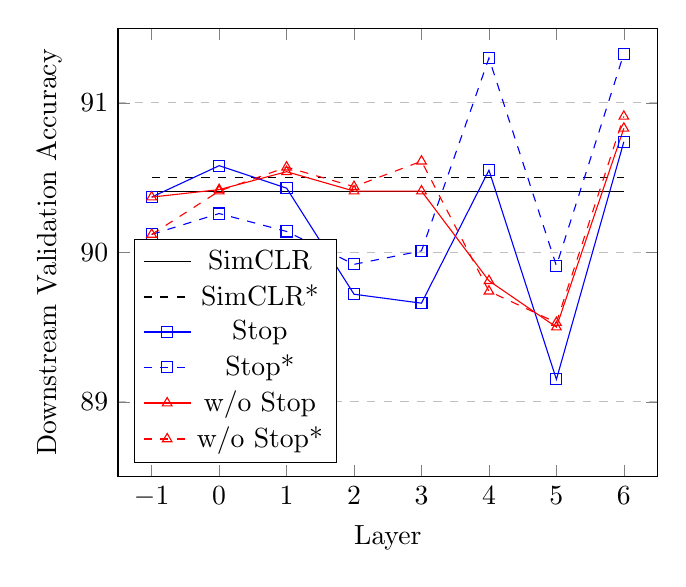
\begin{tikzpicture}
\begin{axis}[
    %title={Temperature dependence of CuSO\(_4\cdot\)5H\(_2\)O solubility},
    % width=0.8\textwidth,
    % height=0.5\textwidth,
    xlabel={Layer},
    ylabel={Downstream Validation Accuracy},
    xmin=-1.5, xmax=6.5,
    ymin=88.5, ymax=91.5,
    xtick={-1,0,1,2,3,4,5,6,7}, %,11,12,13},
    ytick={89,90,91},
    %ytick={0,0.2,0.4,0.6,0.8,1.0}, %,0.6,0.7,0.8,0.9,1.0},
    legend pos=south west,
    ymajorgrids=true,
    grid style=dashed,
]
\addplot[
    color=black,
    %mark=diamond,
    ]
    coordinates {
    % (300,62.14999771118164)(600,63.15999984741211)(900,62.91999816894531)(1200,62.29999923706055)(1500,61.93000030517578)
    (-1,90.40999603271484)
    (0,90.40999603271484)
    (1,90.40999603271484)
    (2,90.40999603271484)
    (3,90.40999603271484)
    (4,90.40999603271484)
    (5,90.40999603271484)
    (6,90.40999603271484)
    
    };
    \addlegendentry{SimCLR}
\addplot[
    %dotted,
    dashed,
    mark options={solid},
    color=black,
    %mark=diamond,
    ]
    coordinates {
    % (300,62.14999771118164)(600,63.15999984741211)(900,62.91999816894531)(1200,62.29999923706055)(1500,61.93000030517578)
    (-1,90.5)
    (0,90.5)
    (1,90.5)
    (2,90.5)
    (3,90.5)
    (4,90.5)
    (5,90.5)
    (6,90.5)
    };
    \addlegendentry{SimCLR*}
\addplot[
    color=blue,
    mark=square,
    ]
    coordinates {
    (-1, 90.3699951171875)
    (0, 90.57999420166016)
    (1, 90.43000030517578)
    (2, 89.72000122070312)
    (3, 89.65999603271484)
    (4, 90.54999542236328)
    (5, 89.1500015258789)
    (6, 90.73999786376953)
    
    % (-1,90.1199951171875)
    % (0, 90.25999450683594)
    % (1, 90.13999938964844)
    % (2, 89.91999816894531)
    % (3, 90.00999450683594)
    % (4, 91.29999542236328)
    % (5, 89.90999603271484)
    % (6, 91.32999420166016)
    };
    \addlegendentry{Stop}
\addplot[
    dashed,
    mark options={solid},
    color=blue,
    mark=square,
    ]
    coordinates {
    (-1,90.1199951171875)
    (0, 90.25999450683594)
    (1, 90.13999938964844)
    (2, 89.91999816894531)
    (3, 90.00999450683594)
    (4, 91.29999542236328)
    (5, 89.90999603271484)
    (6, 91.32999420166016)
    };
    \addlegendentry{Stop*}
\addplot[
    color=red,
    mark=triangle,
    ]
    coordinates {
    (-1, 90.3699951171875)
    (0, 90.41999816894531)
    (1, 90.54000091552734)
    (2, 90.40999603271484)
    (3, 90.40999603271484)
    (4, 89.80999755859375)
    (5, 89.5)
    (6, 90.82999420166016)
    };
    \addlegendentry{w/o Stop}
\addplot[
    dashed,
    mark options={solid},
    color=red,
    mark=triangle,
    ]
    coordinates {
    (-1, 90.1199951171875)
    (0, 90.40999603271484)
    (1, 90.56999969482422)
    (2, 90.43999481201172)
    (3, 90.61000061035156)
    (4, 89.73999786376953)
    (5, 89.52999877929688)
    (6, 90.90999603271484)
    };
    \addlegendentry{w/o Stop*}


\end{axis}
\end{tikzpicture}
}
%\vspace{-.1in}
%\caption{Continue Cifar100-Cifar100}
\caption{Cifar10: Comparing SimCLR with Deep Augmentation with and without stop-gradient. *: Initialized with pre-trained SimCLR model. Stop: short for stop-gradient.}
\label{fig:cifar10-compare}
%\vspace{-0.5cm}
\end{figure}


\begin{figure}[ht]
\centering
\resizebox{1.0\columnwidth}{!}{%
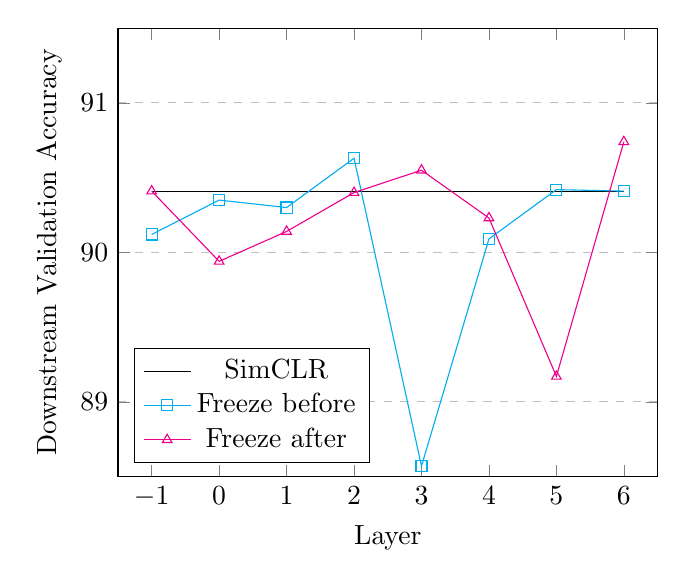
\begin{tikzpicture}
\begin{axis}[
    %title={Temperature dependence of CuSO\(_4\cdot\)5H\(_2\)O solubility},
    % width=0.8\textwidth,
    % height=0.5\textwidth,
    xlabel={Layer},
    ylabel={Downstream Validation Accuracy},
    xmin=-1.5, xmax=6.5,
    ymin=88.5, ymax=91.5,
    xtick={-1,0,1,2,3,4,5,6,7}, %,11,12,13},
    ytick={89,90,91},
    %ytick={0,0.2,0.4,0.6,0.8,1.0}, %,0.6,0.7,0.8,0.9,1.0},
    legend pos=south west,
    ymajorgrids=true,
    grid style=dashed,
]
\addplot[
    color=black,
    %mark=diamond,
    ]
    coordinates {
    % (300,62.14999771118164)(600,63.15999984741211)(900,62.91999816894531)(1200,62.29999923706055)(1500,61.93000030517578)
    (-1,90.40999603271484)
    (0,90.40999603271484)
    (1,90.40999603271484)
    (2,90.40999603271484)
    (3,90.40999603271484)
    (4,90.40999603271484)
    (5,90.40999603271484)
    (6,90.40999603271484)
    
    };
    \addlegendentry{SimCLR}
\addplot[
    color=cyan,
    mark=square,
    ]
    coordinates {
    (-1, 90.1199951171875)
    (0, 90.3499984741211)
    (1, 90.29999542236328)
    (2, 90.62999725341797)
    (3, 88.56999969482422)
    (4, 90.08999633789062)
    (5, 90.41999816894531)
    (6, 90.40999603271484)
    
    % (-1, 90.3699951171875)
    % (0, 90.41999816894531)
    % (1, 90.54000091552734)
    % (2, 90.40999603271484)
    % (3, 90.40999603271484)
    % (4, 89.80999755859375)
    % (5, 89.5)
    % (6, 90.40999603271484) % 90.82999420166016)
    
    % (-1,90.1199951171875)
    % (0, 90.25999450683594)
    % (1, 90.13999938964844)
    % (2, 89.91999816894531)
    % (3, 90.00999450683594)
    % (4, 91.29999542236328)
    % (5, 89.90999603271484)
    % (6, 91.32999420166016)
    };
    \addlegendentry{Freeze before}

\addplot[
    color=magenta,
    mark=triangle,
    ]
    coordinates {
    (-1,90.40999603271484)
    (0, 89.93999481201172)
    (1, 90.13999938964844)
    (2, 90.4000015258789)
    (3, 90.54999542236328)
    (4, 90.22999572753906)
    (5, 89.16999816894531)
    (6, 90.73999786376953)
    };
    \addlegendentry{Freeze after}



\end{axis}
\end{tikzpicture}
}
%\vspace{-.1in}
%\caption{Continue Cifar100-Cifar100}
\caption{Cifar10: Comparing freezing layers before or after Deep Augmentation with stop-gradient, initialized with pre-trained SimCLR model. Note that for "Freeze before" Layer -1 freezes nothing, and for "Freeze after" Layer 6 freezes nothing.}
\label{fig:cifar10-freeze}
%\vspace{-0.5cm}
\end{figure}


\begin{figure}[ht]
\centering
\resizebox{1.0\columnwidth}{!}{%
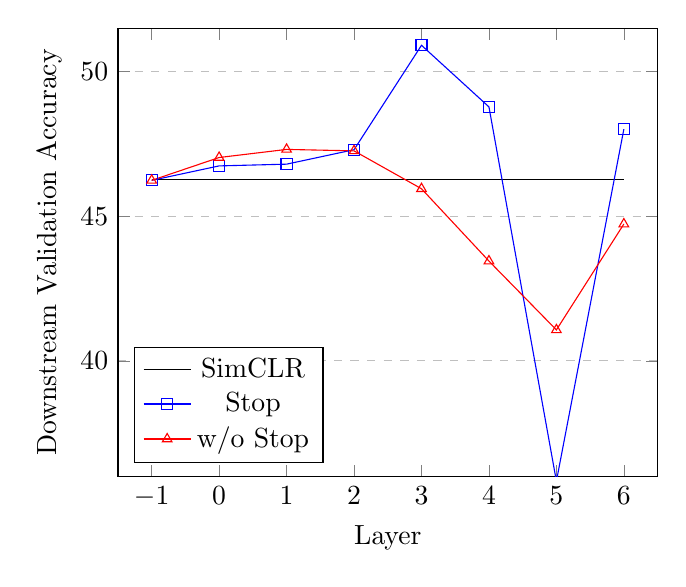
\begin{tikzpicture}
\begin{axis}[
    %title={Temperature dependence of CuSO\(_4\cdot\)5H\(_2\)O solubility},
    % width=0.8\textwidth,
    % height=0.5\textwidth,
    xlabel={Layer},
    ylabel={Downstream Validation Accuracy},
    xmin=-1.5, xmax=6.5,
    ymin=36, ymax=51.5,
    xtick={-1,0,1,2,3,4,5,6,7}, %,11,12,13},
    ytick={40,45,50},
    %ytick={0,0.2,0.4,0.6,0.8,1.0}, %,0.6,0.7,0.8,0.9,1.0},
    legend pos=south west,
    ymajorgrids=true,
    grid style=dashed,
]
\addplot[
    color=black,
    %mark=diamond,
    ]
    coordinates {
    % (300,62.14999771118164)(600,63.15999984741211)(900,62.91999816894531)(1200,62.29999923706055)(1500,61.93000030517578)
    (-1,46.27000045776367)
    (0,46.27000045776367)
    (1,46.27000045776367)
    (2,46.27000045776367)
    (3,46.27000045776367)
    (4,46.27000045776367)
    (5,46.27000045776367)
    (6,46.27000045776367)
    
    };
    \addlegendentry{SimCLR}
\addplot[
    color=blue,
    mark=square,
    ]
    coordinates {
    (-1, 46.23999786376953)
    (0, 46.73999786376953)
    (1, 46.79999923706055)
    (2, 47.29999923706055)
    (3, 50.90999984741211)
    (4, 48.779998779296875)
    (5, 35.84000015258789)
    (6, 48.0099983215332)
    };
    \addlegendentry{Stop}
\addplot[
    color=red,
    mark=triangle,
    ]
    coordinates {
    (-1, 46.23999786376953)
    (0, 47.029998779296875)
    (1, 47.30999755859375)
    (2, 47.2599983215332)
    (3, 45.94999694824219)
    (4, 43.45000076293945)
    (5, 41.06999969482422)
    (6, 44.72999954223633)
    };
    \addlegendentry{w/o Stop}


\end{axis}
\end{tikzpicture}
}
%\vspace{-.1in}
%\caption{Continue Cifar100-Cifar100}
\caption{Finetuning on Cifar100 of networks pre-trained on Cifar10. Comparing SimCLR with Deep Augmentation with and without stop-gradient.}
\label{fig:cifar10-cifar100-domain}
%\vspace{-0.5cm}
\end{figure}

% \subsection{Early Layers and Data Distribution}

% Early layers have fewer parameters to learn to be invariant to these transformations with respect to non-augmented images. This fools the network into believing the data-distribution is different from how it actually looks like at test time; the NN effectively never sees non-augmented data during training, and dropout is not creating realistic looking images as opposed to typical image transformations like cropping.

%Either way, training a NN with dropout should lead to less co-adaptation and in turn make higher layer transformations more useful. 
%This logic suggests that a NN trained with Deep Augmentation at a certain layer may be suitable for further training on a new dataset (optionally frozen up to that layer) using Deep Augmentation at the same layer.
%Future work may investigate ways to optimally train a NN so that dropout serves as a useful higher transformation. 
%}

\subsection{Cifar100 across epochs}
\label{sec:cifar100-across-epochs}


We include results where we finetuned and tested checkpoints at different epochs for various experiments.

In Figure \ref{fig:cifar100-everywhere-vs-layer-epochs}, we include results for dropout everywhere at different rates and 50\% dropout at single layers. 

In Figure \ref{fig:cifar100-with-sg-without-sg-epochs}, we include results for sampling 50\% of each batch and performing 50\% dropout on that sample, with and without stop-gradient. 

In Figure \ref{fig:cifar100-freezingbeforeafter-epochs}, we compare freezing layers before or after Deep Augmentation with stop-gradient initialized with pre-trained SimCLR model. 

In Figure \ref{fig:continue-cifar100-epochs}, we inlcude results for 50\% sampling, 50\% dropout, with and without stop-gradient, and initialized with pre-trained SimCLR model.

\begin{figure}
\begin{subfigure}{.49\columnwidth}
\resizebox{\columnwidth}{!}{%
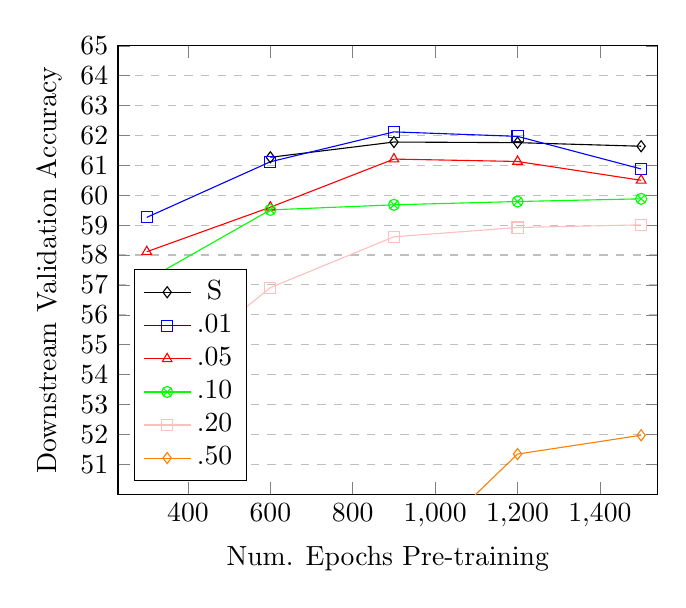
\begin{tikzpicture}
\begin{axis}[
    xlabel={Num. Epochs Pre-training},
    ylabel={Downstream Validation Accuracy},
    xmin=230, xmax=1540,
    ymin=50, ymax=65,
    xtick={200,400,600,800,1000,1200,1400}, %,11,12,13},
    ytick={51,52,53,54,55,56,57,58,59,60,61,62,63,64,65},
    %ytick={0,0.2,0.4,0.6,0.8,1.0}, %,0.6,0.7,0.8,0.9,1.0},
    legend pos=south west,
    ymajorgrids=true,
    grid style=dashed,
]
\addplot[
    color=black,
    mark=diamond,
    ]
    coordinates {
    (600,61.27)(900,61.78)(1200,61.76)(1500,61.64)
    };
    \addlegendentry{S}
\addplot[
    color=blue,
    mark=square,
    ]
    coordinates {
   (300,59.2599983215332)(600,61.119998931884766)(900,62.119998931884766)(1200,61.96999740600586)(1500,60.87999725341797)
    };
    \addlegendentry{.01}
\addplot[
    color=red,
    mark=triangle,
    ]
    coordinates {
    (300,58.1099967956543)(600,59.599998474121094)(900,61.209999084472656)(1200,61.12999725341797)(1500,60.5)
    };
    \addlegendentry{.05}
\addplot[
    color=green,
    mark=otimes,
    ]
    coordinates {
    (300,57.15999984741211)(600,59.5099983215332)(900,59.68000030517578)(1200,59.78999710083008)(1500,59.87999725341797)
    };
    \addlegendentry{.10}
\addplot[
    color=pink,
    mark=square,
    ]
    coordinates {
    (300,53.54999923706055)(600,56.90999984741211)(900,58.6099967956543)(1200,58.91999816894531)(1500,59.0099983215332)
    };
    \addlegendentry{.20}
\addplot[
    color=orange,
    mark=diamond,
    ]
    coordinates {
    (300,37.86000061035156)(600,43.47999954223633)(900,47.349998474121094)(1200,51.34000015258789)(1500,51.96999740600586)
    };
    \addlegendentry{.50}


\end{axis}
\end{tikzpicture}
}
%\vspace{-.1in}
\caption{Dropout at all layers}
\label{fig:drop_everywhere_cifar100} 
\end{subfigure}%
\hspace{0.005\columnwidth}
\begin{subfigure}{.49\columnwidth}
\centering
\resizebox{\columnwidth}{!}{%
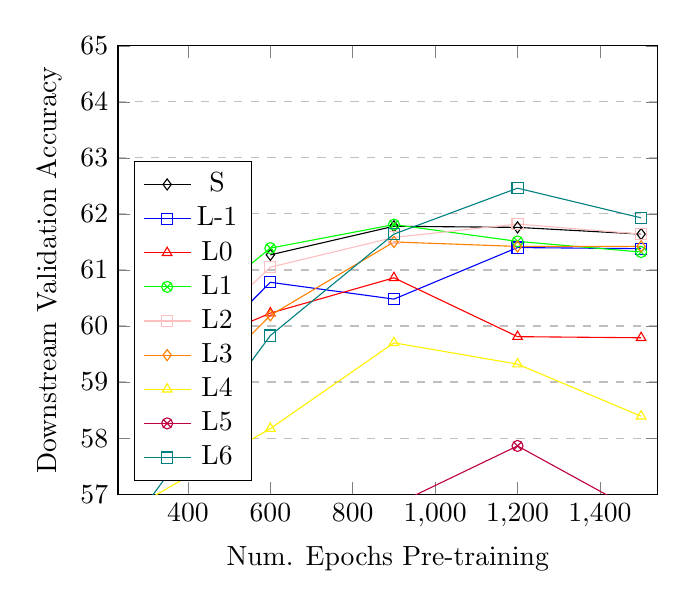
\begin{tikzpicture}
\begin{axis}[
    %title={Temperature dependence of CuSO\(_4\cdot\)5H\(_2\)O solubility},
    % width=0.8\textwidth,
    % height=0.5\textwidth,
    xlabel={Num. Epochs Pre-training},
    ylabel={Downstream Validation Accuracy},
    xmin=230, xmax=1540,
    ymin=57, ymax=65,
    xtick={200,400,600,800,1000,1200,1400}, %,11,12,13},
    ytick={57, 58, 59, 60, 61, 62, 63, 64, 65},
    %ytick={0,0.2,0.4,0.6,0.8,1.0}, %,0.6,0.7,0.8,0.9,1.0},
    legend pos=south west,
    ymajorgrids=true,
    grid style=dashed,
]
\addplot[
    color=black,
    mark=diamond,
    ]
    coordinates {
    (600,61.27)(900,61.78)(1200,61.76)(1500,61.64)
    };
    \addlegendentry{S}

\addplot[
    color=blue,
    mark=square,
    ]
    coordinates {
    (300,58.55999755859375)(600,60.779998779296875)(900,60.47999954223633)(1200,61.39999771118164)(1500,61.37999725341797)
    };
    \addlegendentry{L-1}
\addplot[
    color=red,
    mark=triangle,
    ]
    coordinates {
    (300,59.28999710083008)(600,60.22999954223633)(900,60.8599967956543)(1200,59.80999755859375)(1500,59.78999710083008)
    };
    
    \addlegendentry{L0}
\addplot[
    color=green,
    mark=otimes,
    ]
    coordinates {
    (300,59.59000015258789)(600,61.38999938964844)(900,61.80999755859375)(1200,61.5099983215332)(1500,61.31999969482422)
    };
    
    \addlegendentry{L1}
\addplot[
    color=pink,
    mark=square,
    ]
    coordinates {
    (300,58.94999694824219)(600,61.04999923706055)(900,61.57999801635742)(1200,61.81999969482422)(1500,61.63999938964844)
    
    };
    \addlegendentry{L2}
\addplot[
    color=orange,
    mark=diamond,
    ]
    coordinates {
    (300,57.959999084472656)(600,60.189998626708984)(900,61.5)(1200,61.41999816894531)(1500,61.41999816894531)
    };
    \addlegendentry{L3}
    
\addplot[
    color=yellow,
    mark=triangle,
    ]
    coordinates {
    (300,56.88999938964844)(600,58.16999816894531)(900,59.69999694824219)(1200,59.31999969482422)(1500,58.38999938964844)
    
    };
    \addlegendentry{L4}
\addplot[
    color=purple,
    mark=otimes,
    ]
    coordinates {
    (300,52.099998474121094)(600,55.30999755859375)(900,56.79999923706055)(1200,57.8599967956543)(1500,56.64999771118164)
    };
    
    \addlegendentry{L5}
\addplot[
    color=teal,
    mark=square,
    ]
    coordinates {
    (300,56.84000015258789)(600,59.82999801635742)(900,61.63999938964844)(1200,62.459999084472656)(1500,61.93000030517578)
    };
    \addlegendentry{L6}

\end{axis}
\end{tikzpicture}
}
%\vspace{-.1in}
\caption{50\% dropout at single layer}
\label{fig:trainble-two-sided-cifar100}
\end{subfigure}
\caption{Cifar100. Comparing dropout rates at all layers versus 50\% dropout targeted at a specific layer. Note difference in $y$-axis.}
\label{fig:cifar100-everywhere-vs-layer-epochs}
\end{figure}

\begin{figure}
\begin{subfigure}{.49\columnwidth}
\resizebox{\columnwidth}{!}{%
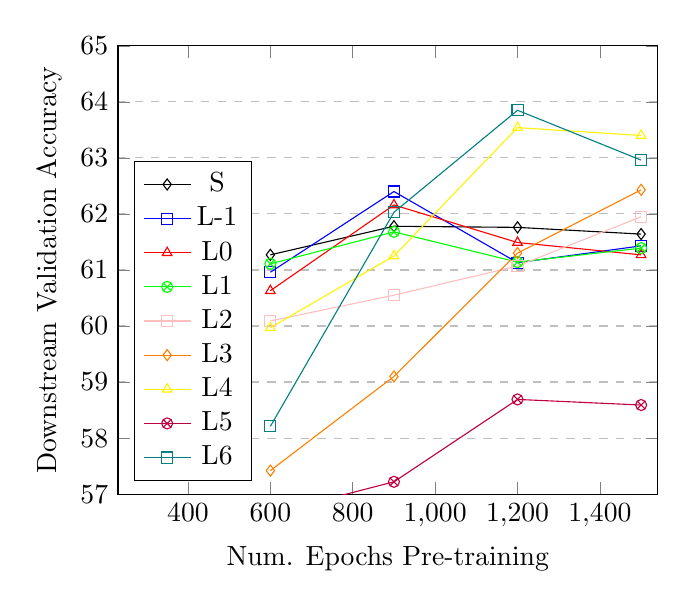
\begin{tikzpicture}
\begin{axis}[
    %title={Temperature dependence of CuSO\(_4\cdot\)5H\(_2\)O solubility},
    % width=0.8\textwidth,
    % height=0.5\textwidth,
    xlabel={Num. Epochs Pre-training},
    ylabel={Downstream Validation Accuracy},
    xmin=230, xmax=1540,
    ymin=57, ymax=65,
    xtick={200,400,600,800,1000,1200,1400}, %,11,12,13},
    ytick={57, 58, 59, 60, 61, 62, 63, 64, 65},
    %ytick={0,0.2,0.4,0.6,0.8,1.0}, %,0.6,0.7,0.8,0.9,1.0},
    legend pos=south west,
    ymajorgrids=true,
    grid style=dashed,
]
\addplot[
    color=black,
    mark=diamond,
    ]
    coordinates {
    (600,61.27)(900,61.78)(1200,61.76)(1500,61.64)
    };
    \addlegendentry{S}
\addplot[
    color=blue,
    mark=square,
    ]
    coordinates {
    (600,60.959999084472656)(900,62.39999771118164)(1200,61.12999725341797)(1500,61.43000030517578)
    };
    \addlegendentry{L-1}
\addplot[
    color=red,
    mark=triangle,
    ]
    coordinates {
    (600,60.62999725341797)(900,62.15999984741211)(1200,61.48999786376953)(1500,61.269996643066406)
    };
    \addlegendentry{L0}
\addplot[
    color=green,
    mark=otimes,
    ]
    coordinates {
    (600,61.1099967956543)(900,61.68000030517578)(1200,61.13999938964844)(1500,61.38999938964844)
    };
    \addlegendentry{L1}
\addplot[
    color=pink,
    mark=square,
    ]
    coordinates {
    (600,60.09000015258789)(900,60.54999923706055)(1200,61.06999969482422)(1500,61.94999694824219)
    };
    \addlegendentry{L2}
\addplot[
    color=orange,
    mark=diamond,
    ]
    coordinates {
    (600,57.41999816894531)(900,59.099998474121094)(1200,61.29999923706055)(1500,62.43000030517578)
    };
    \addlegendentry{L3}
\addplot[
    color=yellow,
    mark=triangle,
    ]
    coordinates {
    (600,59.96999740600586)(900,61.25)(1200,63.53999710083008)(1500,63.39999771118164)
    };
    \addlegendentry{L4}
\addplot[
    color=purple,
    mark=otimes,
    ]
    coordinates {
    (600,56.64999771118164)(900,57.21999740600586)(1200,58.689998626708984)(1500,58.59000015258789)
    };
    \addlegendentry{L5}
\addplot[
    color=teal,
    mark=square,
    ]
    coordinates {
    (600,58.209999084472656)(900,62.029998779296875)(1200,63.849998474121094)(1500,62.959999084472656)
    };
    \addlegendentry{L6}
% \addplot[
%     color=green,
%     mark=square,
%     ]
%     coordinates {
%     (300,55.84000015258789)(600,59.32999801635742)(900,61.41999816894531)(1200,62.869998931884766)(1500,63.56999969482422)
%     };
%     \addlegendentry{L4L6}

% \addplot[
%     color=brown,
%     mark=square,
%     ]
%     coordinates {
%     (300,56.28999710083008)(600,59.189998626708984)(900,62.6099967956543)(1200,62.82999801635742)(1500,62.89999771118164)
%     };
%     \addlegendentry{L4}

    

\end{axis}
\end{tikzpicture}
%\vspace{-.1in}

}
\caption{With stop-gradient}
\label{fig:cifar100-cifar100}
\end{subfigure}%
\hspace{0.005\columnwidth}
\begin{subfigure}{.49\columnwidth}
\centering
\resizebox{\columnwidth}{!}{%
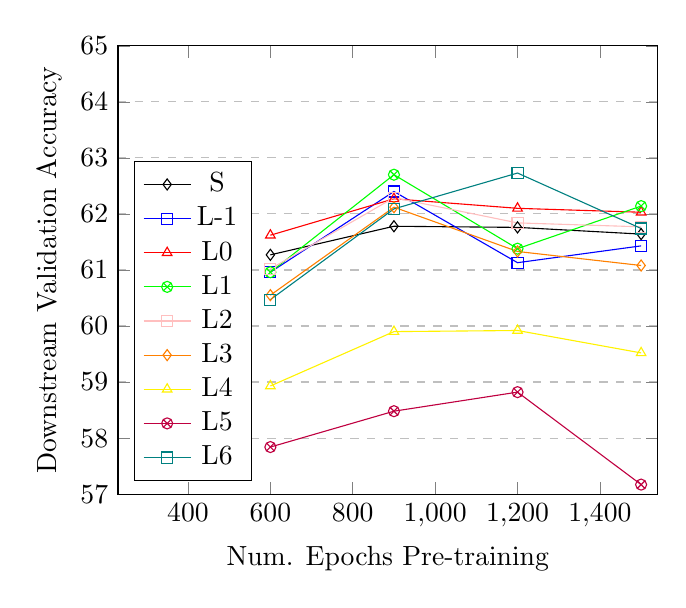
\begin{tikzpicture}
\begin{axis}[
    %title={Temperature dependence of CuSO\(_4\cdot\)5H\(_2\)O solubility},
    % width=0.8\textwidth,
    % height=0.5\textwidth,
    xlabel={Num. Epochs Pre-training},
    ylabel={Downstream Validation Accuracy},
    xmin=230, xmax=1540,
    ymin=57, ymax=65,
    xtick={200,400,600,800,1000,1200,1400}, %,11,12,13},
    ytick={57, 58, 59, 60, 61, 62, 63, 64, 65},
    %ytick={0,0.2,0.4,0.6,0.8,1.0}, %,0.6,0.7,0.8,0.9,1.0},
    legend pos=south west,
    ymajorgrids=true,
    grid style=dashed,
]
\addplot[
    color=black,
    mark=diamond,
    ]
    coordinates {
    (600,61.27)(900,61.78)(1200,61.76)(1500,61.64)
    };
    \addlegendentry{S}
\addplot[
    color=blue,
    mark=square,
    ]
    coordinates {
    (600,60.959999084472656)(900,62.39999771118164)(1200,61.12999725341797)(1500,61.43000030517578)
    };
    \addlegendentry{L-1}
\addplot[
    color=red,
    mark=triangle,
    ]
    coordinates {
    (600,61.619998931884766)(900,62.269996643066406)(1200,62.099998474121094)(1500,62.029998779296875)
    };
    \addlegendentry{L0}
\addplot[
    color=green,
    mark=otimes,
    ]
    coordinates {
    (600,60.959999084472656)(900,62.69999694824219)(1200,61.37999725341797)(1500,62.13999938964844)
    };
    \addlegendentry{L1}
\addplot[
    color=pink,
    mark=square,
    ]
    coordinates {
    (600,61.019996643066406)(900,62.28999710083008)(1200,61.84000015258789)(1500,61.769996643066406)
    };
    \addlegendentry{L2}
\addplot[
    color=orange,
    mark=diamond,
    ]
    coordinates {
    (600,60.54999923706055)(900,62.119998931884766)(1200,61.32999801635742)(1500,61.07999801635742)
    };
    \addlegendentry{L3}
\addplot[
    color=yellow,
    mark=triangle,
    ]
    coordinates {
    (600,58.93000030517578)(900,59.89999771118164)(1200,59.91999816894531)(1500,59.519996643066406)
    };
    \addlegendentry{L4}
\addplot[
    color=purple,
    mark=otimes,
    ]
    coordinates {
    (600,57.84000015258789)(900,58.47999954223633)(1200,58.81999969482422)(1500,57.16999816894531)
    };
    \addlegendentry{L5}
\addplot[
    color=teal,
    mark=square,
    ]
    coordinates {
    (600,60.46999740600586)(900,62.09000015258789)(1200,62.72999954223633)(1500,61.73999786376953)
    };
    \addlegendentry{L6}

% \addplot[
%     color=teal,
%     mark=square,
%     ]
%     coordinates {
%     (300,58.599998474121094)(600,61.279998779296875)(900,62.62999725341797)(1200,62.14999771118164)(1500,61.91999816894531)
%     };
%     \addlegendentry{L6}

    

\end{axis}
\end{tikzpicture}
%\vspace{-.1in}

}
%\vspace{-.1in}
\caption{Without stop-gradient}
\label{fig:trainble-cifar100-cifar100}
\end{subfigure}
\caption{Cifar100. Comparing sampling 50\% and applying 50\% dropout, with or without stop-gradient.}
\label{fig:cifar100-with-sg-without-sg-epochs}
\end{figure}



\begin{figure}
\begin{subfigure}{.49\columnwidth}
  \centering
  \resizebox{1.0\columnwidth}{!}{
  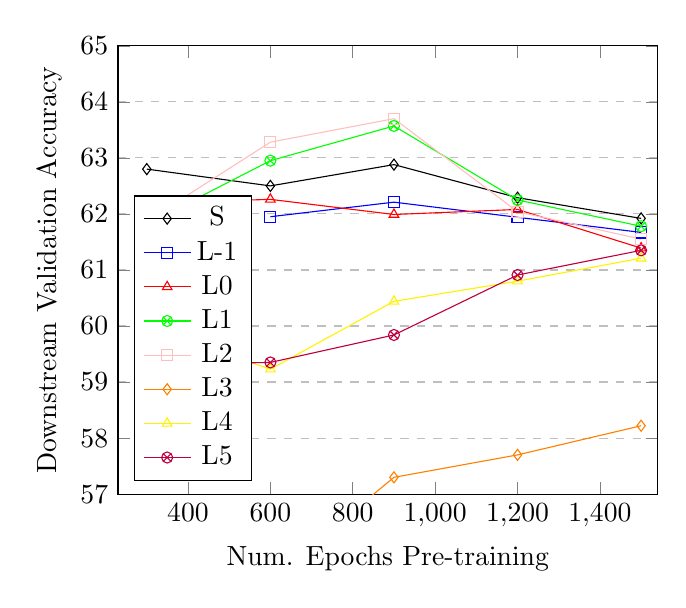
\begin{tikzpicture}
\begin{axis}[
    %title={Temperature dependence of CuSO\(_4\cdot\)5H\(_2\)O solubility},
    % width=0.8\textwidth,
    % height=0.5\textwidth,
    xlabel={Num. Epochs Pre-training},
    ylabel={Downstream Validation Accuracy},
    xmin=230, xmax=1540,
    ymin=57, ymax=65,
    xtick={200,400,600,800,1000,1200,1400}, %,11,12,13},
    ytick={57, 58, 59, 60, 61, 62, 63, 64, 65},
    %ytick={0,0.2,0.4,0.6,0.8,1.0}, %,0.6,0.7,0.8,0.9,1.0},
    legend pos=south west,
    ymajorgrids=true,
    grid style=dashed,
]
\addplot[
    color=black,
    mark=diamond,
    ]
    coordinates {
    (300,62.79999923706055)(600,62.5)(900,62.87999725341797)(1200,62.28999710083008)(1500,61.91999816894531)
    };
    \addlegendentry{S}
\addplot[
    color=blue,
    mark=square,
    ]
    coordinates {
    (600,61.94999694824219)(900,62.209999084472656)(1200,61.939998626708984)(1500,61.66999816894531)
    %(300,60.39999771118164)(600,61.98999786376953)(900,62.3599967956543)(1200,61.73999786376953)(1500,61.7599983215332)
    };
    \addlegendentry{L-1}
\addplot[
    color=red,
    mark=triangle,
    ]
    coordinates {
    (300,62.189998626708984)(600,62.2599983215332)(900,61.98999786376953)(1200,62.07999801635742)(1500,61.38999938964844)
    %(300,61.03999710083008)(600,62.3599967956543)(900,62.1099967956543)(1200,62.43000030517578)(1500,61.769996643066406)
    
    };
    \addlegendentry{L0}
\addplot[
    color=green,
    mark=otimes,
    ]
    coordinates {
    (300,61.81999969482422)(600,62.94999694824219)(900,63.56999969482422)(1200,62.25)(1500,61.779998779296875)
    %(300,62.28999710083008)(600,62.869998931884766)(900,63.439998626708984)(1200,63.09000015258789)(1500,62.0099983215332)
    
    };
    \addlegendentry{L1}
\addplot[
    color=pink,
    mark=square,
    ]
    coordinates {
    (300,61.869998931884766)(600,63.279998779296875)(900,63.69999694824219)(1200,62.03999710083008)(1500,61.54999923706055)
    %(300,62.16999816894531)(600,62.959999084472656)(900,62.21999740600586)(1200,61.459999084472656)(1500,61.40999984741211)
    
    };
    \addlegendentry{L2}
\addplot[
    color=orange,
    mark=diamond,
    ]
    coordinates {
    (300,55.57999801635742)(600,55.46999740600586)(900,57.29999923706055)(1200,57.69999694824219)(1500,58.21999740600586)
    
    };
    \addlegendentry{L3}
\addplot[
    color=yellow,
    mark=triangle,
    ]
    coordinates {
    (300,59.97999954223633)(600,59.22999954223633)(900,60.439998626708984)(1200,60.79999923706055)(1500,61.209999084472656)
    
    };
    \addlegendentry{L4}
\addplot[
    color=purple,
    mark=otimes,
    ]
    coordinates {
    (300,59.30999755859375)(600,59.349998474121094)(900,59.84000015258789)(1200,60.90999984741211)(1500,61.349998474121094)
    
    };
    \addlegendentry{L5}
% \addplot[
%     color=teal,
%     mark=square,
%     ]
%     coordinates {
%     (300,59.599998474121094)(600,59.28999710083008)(900,60.30999755859375)(1200,60.63999938964844)(1500,61.07999801635742)
%     % (300,59.63999938964844)(600,60.80999755859375)(900,62.57999801635742)(1200,64.29000091552734)(1500,64.18999481201172)
%     };
%     \addlegendentry{25}

\end{axis}
\end{tikzpicture}
}
%\caption{Freeze Continue Cifar100-Cifar100}
\caption{Freeze layers before Deep Augmentation}
\label{fig:freeze-continue-cifar100-cifar100}
\end{subfigure}%
\hspace{0.005\columnwidth}
\begin{subfigure}{.49\columnwidth}
  \centering
  \resizebox{1.0\columnwidth}{!}{
\centering
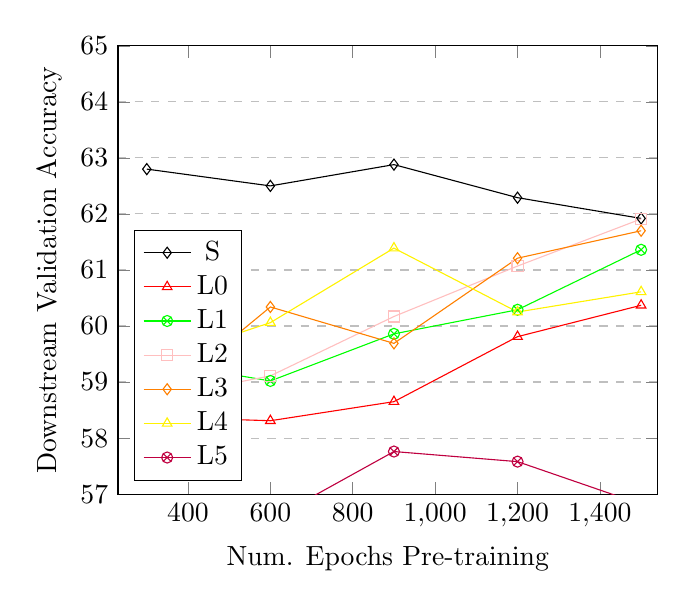
\begin{tikzpicture}
\begin{axis}[
    %title={Temperature dependence of CuSO\(_4\cdot\)5H\(_2\)O solubility},
    % width=0.8\textwidth,
    % height=0.5\textwidth,
    xlabel={Num. Epochs Pre-training},
    ylabel={Downstream Validation Accuracy},
    xmin=230, xmax=1540,
    ymin=57, ymax=65,
    xtick={200,400,600,800,1000,1200,1400}, %,11,12,13},
    ytick={57, 58, 59, 60, 61, 62, 63, 64, 65},
    %ytick={0,0.2,0.4,0.6,0.8,1.0}, %,0.6,0.7,0.8,0.9,1.0},
    legend pos=south west,
    ymajorgrids=true,
    grid style=dashed,
]
\addplot[
    color=black,
    mark=diamond,
    ]
    coordinates {
    (300,62.79999923706055)(600,62.5)(900,62.87999725341797)(1200,62.28999710083008)(1500,61.91999816894531)
    };
    \addlegendentry{S}
% \addplot[
%     color=blue,
%     mark=square,
%     ]
%     coordinates {
%     (600,61.94999694824219)(900,62.209999084472656)(1200,61.939998626708984)(1500,61.66999816894531)
%     };
%     \addlegendentry{L-1}
\addplot[
    color=red,
    mark=triangle,
    ]
    coordinates {
    (300,58.37999725341797)(600,58.30999755859375)(900,58.64999771118164)(1200,59.80999755859375)(1500,60.369998931884766)
    };
    \addlegendentry{L0}
\addplot[
    color=green,
    mark=otimes,
    ]
    coordinates {
    (300,59.38999938964844)(600,59.019996643066406)(900,59.8599967956543)(1200,60.28999710083008)(1500,61.3599967956543)
    };
    \addlegendentry{L1}
\addplot[
    color=pink,
    mark=square,
    ]
    coordinates {
    (300,58.68000030517578)(600,59.1099967956543)(900,60.16999816894531)(1200,61.06999969482422)(1500,61.90999984741211)
    };
    \addlegendentry{L2}
\addplot[
    color=orange,
    mark=diamond,
    ]
    coordinates {
    (300,58.519996643066406)(600,60.34000015258789)(900,59.689998626708984)(1200,61.209999084472656)(1500,61.69999694824219)
    };
    \addlegendentry{L3}
\addplot[
    color=yellow,
    mark=triangle,
    ]
    coordinates {
    (300,59.32999801635742)(600,60.05999755859375)(900,61.38999938964844)(1200,60.25)(1500,60.6099967956543)
    };
    \addlegendentry{L4}
\addplot[
    color=purple,
    mark=otimes,
    ]
    coordinates {
    (300,56.07999801635742)(600,56.53999710083008)(900,57.7599983215332)(1200,57.57999801635742)(1500,56.81999969482422)
    
    
    };
    \addlegendentry{L5}
% \addplot[
%     color=teal,
%     mark=square,
%     ]
%     coordinates {
%     (300,61.63999938964844)(600,61.97999954223633)(900,62.91999816894531)(1200,62.62999725341797)(1500,61.5099983215332)
%     };
%     \addlegendentry{L6}

\end{axis}
\end{tikzpicture}
}
%\vspace{-.1in}
%\caption{Continue Freeze Reverse Cifar100-Cifar100}
\caption{Freeze layers after Deep Augmentation}
\label{fig:freeze-reverse-continue-cifar100-cifar100}
\end{subfigure}
\caption{Cifar100. Comparing freezing layers before or after Deep Augmentation with stop-gradient initialized with pre-trained SimCLR model.}
\label{fig:cifar100-freezingbeforeafter-epochs}
\end{figure}




\begin{figure}
\begin{subfigure}{.49\columnwidth}
  \centering
  \resizebox{1.0\columnwidth}{!}{
  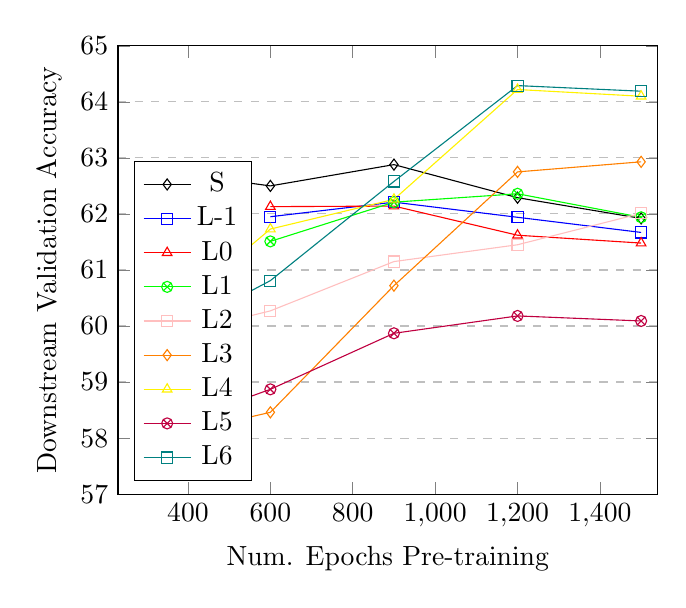
\begin{tikzpicture}
\begin{axis}[
    %title={Temperature dependence of CuSO\(_4\cdot\)5H\(_2\)O solubility},
    % width=0.8\textwidth,
    % height=0.5\textwidth,
    xlabel={Num. Epochs Pre-training},
    ylabel={Downstream Validation Accuracy},
    xmin=230, xmax=1540,
    ymin=57, ymax=65,
    xtick={200,400,600,800,1000,1200,1400}, %,11,12,13},
    ytick={57, 58, 59, 60, 61, 62, 63, 64, 65},
    %ytick={0,0.2,0.4,0.6,0.8,1.0}, %,0.6,0.7,0.8,0.9,1.0},
    legend pos=south west,
    ymajorgrids=true,
    grid style=dashed,
]
\addplot[
    color=black,
    mark=diamond,
    ]
    coordinates {
    % (300,62.14999771118164)(600,63.15999984741211)(900,62.91999816894531)(1200,62.29999923706055)(1500,61.93000030517578)
    (300,62.79999923706055)(600,62.5)(900,62.87999725341797)(1200,62.28999710083008)(1500,61.91999816894531)
    };
    \addlegendentry{S}
\addplot[
    color=blue,
    mark=square,
    ]
    coordinates {
    (600,61.94999694824219)(900,62.209999084472656)(1200,61.939998626708984)(1500,61.66999816894531)
    %(300,60.39999771118164)(600,61.98999786376953)(900,62.3599967956543)(1200,61.73999786376953)(1500,61.7599983215332)
    };
    \addlegendentry{L-1}
\addplot[
    color=red,
    mark=triangle,
    ]
    coordinates {
    (600,62.12999725341797)(900,62.13999938964844)(1200,61.619998931884766)(1500,61.47999954223633)
    %(300,60.779998779296875)(600,61.3599967956543)(900,62.15999984741211)(1200,61.119998931884766)(1500,60.91999816894531)
    };
    \addlegendentry{L0}
\addplot[
    color=green,
    mark=otimes,
    ]
    coordinates {
    (600,61.5099983215332)(900,62.209999084472656)(1200,62.3599967956543)(1500,61.939998626708984)
    %(300,60.119998931884766)(600,61.30999755859375)(900,62.769996643066406)(1200,61.619998931884766)(1500,61.80999755859375)
    };
    
    \addlegendentry{L1}
\addplot[
    color=pink,
    mark=square,
    ]
    coordinates {
    (300,59.72999954223633)(600,60.269996643066406)(900,61.14999771118164)(1200,61.44999694824219)(1500,62.0099983215332)
    %(300,59.72999954223633)(600,60.269996643066406)(900,61.14999771118164)(1200,61.44999694824219)(1500,62.0099983215332)
    };
    \addlegendentry{L2}
\addplot[
    color=orange,
    mark=diamond,
    ]
    coordinates {
    (300,57.94999694824219)(600,58.459999084472656)(900,60.71999740600586)(1200,62.75)(1500,62.93000030517578)
    };
    \addlegendentry{L3}
\addplot[
    color=yellow,
    mark=triangle,
    ]
    coordinates {
    (300,59.869998931884766)(600,61.72999954223633)(900,62.2599983215332)(1200,64.22000122070312)(1500,64.0999984741211)
    };
    \addlegendentry{L4}
\addplot[
    color=purple,
    mark=otimes,
    ]
    coordinates {
    (300,58.07999801635742)(600,58.869998931884766)(900,59.869998931884766)(1200,60.18000030517578)(1500,60.09000015258789)
    };
    \addlegendentry{L5}
\addplot[
    color=teal,
    mark=square,
    ]
    coordinates {
    (300,59.63999938964844)(600,60.80999755859375)(900,62.57999801635742)(1200,64.29000091552734)(1500,64.18999481201172)
    };
    \addlegendentry{L6}

\end{axis}
\end{tikzpicture}
}
\caption{With stop-gradient.}
\label{fig:continue-cifar100-cifar100}
\end{subfigure}%
\hspace{0.005\columnwidth}
\begin{subfigure}{.49\columnwidth}
  \centering
  \resizebox{1.0\columnwidth}{!}{
\centering
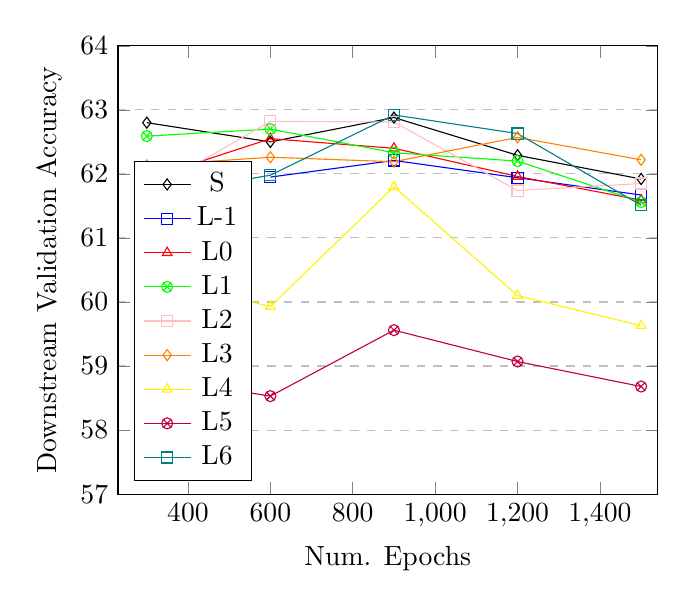
\begin{tikzpicture}
\begin{axis}[
    %title={Temperature dependence of CuSO\(_4\cdot\)5H\(_2\)O solubility},
    % width=0.8\textwidth,
    % height=0.5\textwidth,
    xlabel={Num. Epochs},
    ylabel={Downstream Validation Accuracy},
    xmin=230, xmax=1540,
    ymin=57, ymax=64,
    xtick={200,400,600,800,1000,1200,1400}, %,11,12,13},
    ytick={57, 58, 59, 60, 61, 62, 63, 64},
    %ytick={0,0.2,0.4,0.6,0.8,1.0}, %,0.6,0.7,0.8,0.9,1.0},
    legend pos=south west,
    ymajorgrids=true,
    grid style=dashed,
]
\addplot[
    color=black,
    mark=diamond,
    ]
    coordinates {
    (300,62.79999923706055)(600,62.5)(900,62.87999725341797)(1200,62.28999710083008)(1500,61.91999816894531)
    };
    \addlegendentry{S}
\addplot[
    color=blue,
    mark=square,
    ]
    coordinates {
    (600,61.94999694824219)(900,62.209999084472656)(1200,61.939998626708984)(1500,61.66999816894531)
    };
    \addlegendentry{L-1}
\addplot[
    color=red,
    mark=triangle,
    ]
    coordinates {
    (300,61.91999816894531)(600,62.54999923706055)(900,62.39999771118164)(1200,61.959999084472656)(1500,61.59000015258789)
    };
    \addlegendentry{L0}
\addplot[
    color=green,
    mark=otimes,
    ]
    coordinates {
    (300,62.59000015258789)(600,62.69999694824219)(900,62.32999801635742)(1200,62.19999694824219)(1500,61.55999755859375)
    };
    \addlegendentry{L1}
\addplot[
    color=pink,
    mark=square,
    ]
    coordinates {
    (300,61.709999084472656)(600,62.81999969482422)(900,62.80999755859375)(1200,61.73999786376953)(1500,61.849998474121094)
    };
    \addlegendentry{L2}
\addplot[
    color=orange,
    mark=diamond,
    ]
    coordinates {
    (300,62.12999725341797)(600,62.2599983215332)(900,62.189998626708984)(1200,62.56999969482422)(1500,62.21999740600586)
    };
    \addlegendentry{L3}
\addplot[
    color=yellow,
    mark=triangle,
    ]
    coordinates {
    (300,60.37999725341797)(600,59.93000030517578)(900,61.79999923706055)(1200,60.099998474121094)(1500,59.62999725341797)
    };
    \addlegendentry{L4}
\addplot[
    color=purple,
    mark=otimes,
    ]
    coordinates {
    (300,58.84000015258789)(600,58.529998779296875)(900,59.55999755859375)(1200,59.06999969482422)(1500,58.68000030517578)
    };
    \addlegendentry{L5}
\addplot[
    color=teal,
    mark=square,
    ]
    coordinates {
    (300,61.63999938964844)(600,61.97999954223633)(900,62.91999816894531)(1200,62.62999725341797)(1500,61.5099983215332)
    };
    \addlegendentry{L6}

\end{axis}
\end{tikzpicture}
%\vspace{-.1in}
}
\caption{Without stop-gradient.}
\label{fig:random_erdos}
\end{subfigure}
\caption{Cifar100. 50\% sampling, 50\% dropout, with and without stop-gradient, and initialized with pre-trained SimCLR model.}
\label{fig:continue-cifar100-epochs}
\end{figure}

%%%%%%%%%%%%


\subsection{Cifar10 across epochs}
\label{sec:cifar10-across-epochs}

We include results where we finetuned and tested checkpoints at different epochs for various experiments.

In Figure \ref{fig:cifar10-everywhere-vs-layer-epochs}, we include results for dropout everywhere at different rates and 50\% dropout at single layers. 

In Figure \ref{fig:cifar10-with-sg-without-sg-epochs}, we include results for sampling 50\% of each batch and performing 50\% dropout on that sample, with and without stop-gradient. 

In Figure \ref{fig:cifar10-freezingbeforeafter-epochs}, we compare freezing layers before or after Deep Augmentation with stop-gradient initialized with pre-trained SimCLR model. 

In Figure \ref{fig:continue-cifar10-epochs}, we inlcude results for 50\% sampling, 50\% dropout, with and without stop-gradient, and initialized with pre-trained SimCLR model.



\begin{figure}
\begin{subfigure}{.49\columnwidth}
\resizebox{\columnwidth}{!}{%
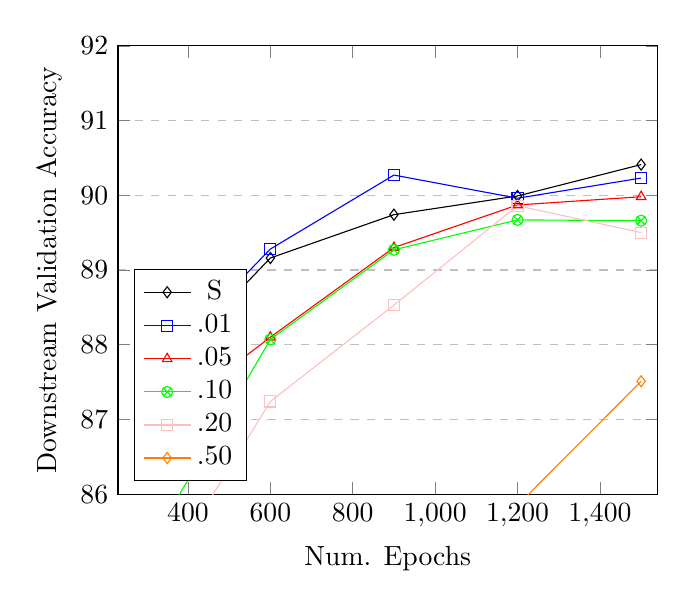
\begin{tikzpicture}
\begin{axis}[
    %title={Temperature dependence of CuSO\(_4\cdot\)5H\(_2\)O solubility},
    % width=0.8\textwidth,
    % height=0.5\textwidth,
    xlabel={Num. Epochs},
    ylabel={Downstream Validation Accuracy},
    xmin=230, xmax=1540,
    ymin=86, ymax=92,
    xtick={200,400,600,800,1000,1200,1400}, %,11,12,13},
    ytick={86,87,88,89,90,91,92},
    %ytick={0,0.2,0.4,0.6,0.8,1.0}, %,0.6,0.7,0.8,0.9,1.0},
    legend pos=south west,
    ymajorgrids=true,
    grid style=dashed,
]
\addplot[
    color=black,
    mark=diamond,
    ]
    coordinates {
    (300,87.43000030517578)(600,89.15999603271484)(900,89.73999786376953)(1200,89.98999786376953)(1500,90.40999603271484)
    };
    \addlegendentry{S}
\addplot[
    color=blue,
    mark=square,
    ]
    coordinates {
   (300,87.56999969482422)(600,89.27999877929688)(900,90.2699966430664)(1200,89.95999908447266)(1500,90.22999572753906)
    };
    \addlegendentry{.01}
    
\addplot[
    color=red,
    mark=triangle,
    ]
    coordinates {
    (300,86.83999633789062)(600,88.0999984741211)(900,89.29999542236328)(1200,89.8699951171875)(1500,89.97999572753906)
    };
    
    \addlegendentry{.05}
\addplot[
    color=green,
    mark=otimes,
    ]
    coordinates {
    (300,85.25)(600,88.06999969482422)(900,89.2699966430664)(1200,89.66999816894531)(1500,89.65999603271484)
    };
    
    \addlegendentry{.10}
\addplot[
    color=pink,
    mark=square,
    ]
    coordinates {
    (300,84.55999755859375)(600,87.23999786376953)(900,88.52999877929688)(1200,89.86000061035156)(1500,89.5)
    
    };
    \addlegendentry{.20}
\addplot[
    color=orange,
    mark=diamond,
    ]
    coordinates {
    (300,76.54999542236328)(600,80.56999969482422)(900,82.98999786376953)(1200,85.8499984741211)(1500,87.50999450683594)
    
    };
    \addlegendentry{.50}

\end{axis}
\end{tikzpicture}
%\vspace{-.1in}

}
\caption{Dropout at all layers}
\label{fig:cifar10-drop-everywhere-epochs}
\end{subfigure}%
\hspace{0.005\columnwidth}
\begin{subfigure}{.49\columnwidth}
\centering
\resizebox{\columnwidth}{!}{%

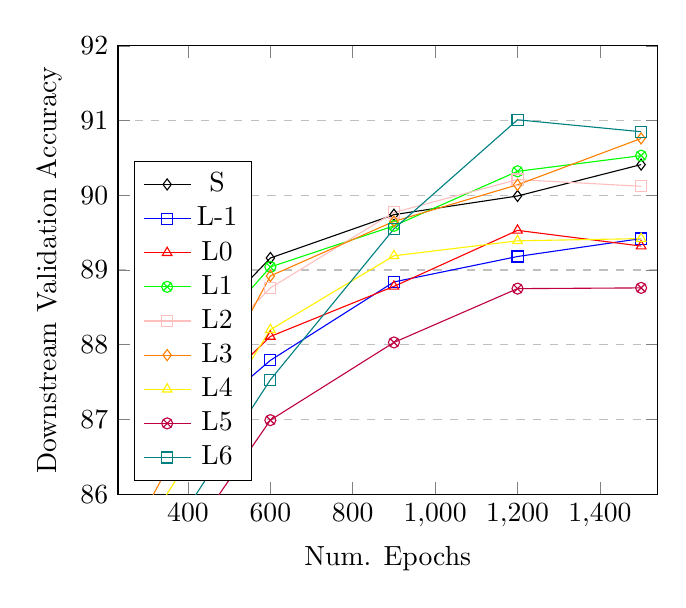
\begin{tikzpicture}
\begin{axis}[
    %title={Temperature dependence of CuSO\(_4\cdot\)5H\(_2\)O solubility},
    % width=0.8\textwidth,
    % height=0.5\textwidth,
    xlabel={Num. Epochs},
    ylabel={Downstream Validation Accuracy},
    xmin=230, xmax=1540,
    ymin=86, ymax=92,
    xtick={200,400,600,800,1000,1200,1400}, %,11,12,13},
    ytick={86,87,88,89,90,91,92},
    %ytick={0,0.2,0.4,0.6,0.8,1.0}, %,0.6,0.7,0.8,0.9,1.0},
    legend pos=south west,
    ymajorgrids=true,
    grid style=dashed,
]
\addplot[
    color=black,
    mark=diamond,
    ]
    coordinates {
    (300,87.43000030517578)(600,89.15999603271484)(900,89.73999786376953)(1200,89.98999786376953)(1500,90.40999603271484)
    };
    \addlegendentry{S}

\addplot[
    color=blue,
    mark=square,
    ]
    coordinates {
    (300,86.37999725341797)(600,87.79000091552734)(900,88.83999633789062)(1200,89.18000030517578)(1500,89.41999816894531)
    };
    
    \addlegendentry{L-1}
\addplot[
    color=red,
    mark=triangle,
    ]
    coordinates {
    (300,86.50999450683594)(600,88.11000061035156)(900,88.77999877929688)(1200,89.52999877929688)(1500,89.31999969482422)
    };
    
    \addlegendentry{L0}
\addplot[
    color=green,
    mark=otimes,
    ]
    coordinates {
    (300,87.15999603271484)(600,89.04000091552734)(900,89.58999633789062)(1200,90.31999969482422)(1500,90.52999877929688)
    };
    
    \addlegendentry{L1}
\addplot[
    color=pink,
    mark=square,
    ]
    coordinates {
    (300,87.06999969482422)(600,88.75999450683594)(900,89.7699966430664)(1200,90.20999908447266)(1500,90.1199951171875)
    
    };
    \addlegendentry{L2}
\addplot[
    color=orange,
    mark=diamond,
    ]
    coordinates {
    (300,85.82999420166016)(600,88.91999816894531)(900,89.6500015258789)(1200,90.13999938964844)(1500,90.75999450683594)
    
    };
    \addlegendentry{L3}
    
\addplot[
    color=yellow,
    mark=triangle,
    ]
    coordinates {
    (300,85.56999969482422)(600,88.19999694824219)(900,89.18999481201172)(1200,89.38999938964844)(1500,89.41999816894531)
    
    };
    \addlegendentry{L4}
\addplot[
    color=purple,
    mark=otimes,
    ]
    coordinates {
    (300,84.58999633789062)(600,86.98999786376953)(900,88.02999877929688)(1200,88.75)(1500,88.75999450683594)
    };
    
    \addlegendentry{L5}
\addplot[
    color=teal,
    mark=square,
    ]
    coordinates {
    (300,84.97999572753906)(600,87.52999877929688)(900,89.54999542236328)(1200,91.00999450683594)(1500,90.8499984741211)
    };
    
    \addlegendentry{L6}

\end{axis}
\end{tikzpicture}
    
}
%\vspace{-.1in}
\caption{50\% dropout at single layer}
\label{fig:trainble-two-sided-cifar10}
\end{subfigure}
\caption{Cifar10. Comparing dropout rates at all layers versus 50\% dropout targeted at a specific layer. Note difference in $y$-axis.}
\label{fig:cifar10-everywhere-vs-layer-epochs}
\end{figure}


\begin{figure}
\begin{subfigure}{.49\columnwidth}
\resizebox{\columnwidth}{!}{%
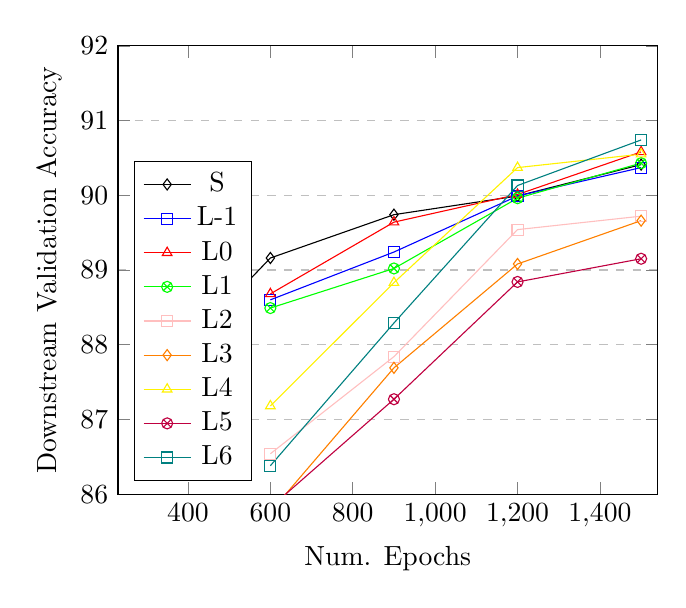
\begin{tikzpicture}
\begin{axis}[
    %title={Temperature dependence of CuSO\(_4\cdot\)5H\(_2\)O solubility},
    % width=0.8\textwidth,
    % height=0.5\textwidth,
    xlabel={Num. Epochs},
    ylabel={Downstream Validation Accuracy},
    xmin=230, xmax=1540,
    ymin=86, ymax=92,
    xtick={200,400,600,800,1000,1200,1400}, %,11,12,13},
    ytick={86,87,88,89,90,91,92},
    %ytick={0,0.2,0.4,0.6,0.8,1.0}, %,0.6,0.7,0.8,0.9,1.0},
    legend pos=south west,
    ymajorgrids=true,
    grid style=dashed,
]
\addplot[
    color=black,
    mark=diamond,
    ]
    coordinates {
    (300,87.43000030517578)(600,89.15999603271484)(900,89.73999786376953)(1200,89.98999786376953)(1500,90.40999603271484)
    };
    \addlegendentry{S}

\addplot[
    color=blue,
    mark=square,
    ]
    coordinates {
    (600,88.5999984741211)(900,89.23999786376953)(1200,89.98999786376953)(1500,90.3699951171875)
    };
    \addlegendentry{L-1}
\addplot[
    color=red,
    mark=triangle,
    ]
    coordinates {
    (600,88.68000030517578)(900,89.63999938964844)(1200,90.00999450683594)(1500,90.57999420166016)
    };
    
    \addlegendentry{L0}
\addplot[
    color=green,
    mark=otimes,
    ]
    coordinates {
    (600,88.48999786376953)(900,89.0199966430664)(1200,89.95999908447266)(1500,90.43000030517578)
    };
    
    \addlegendentry{L1}
\addplot[
    color=pink,
    mark=square,
    ]
    coordinates {
    (600,86.54000091552734)(900,87.83999633789062)(1200,89.54000091552734)(1500,89.72000122070312)
    };
    
    \addlegendentry{L2}
\addplot[
    color=orange,
    mark=diamond,
    ]
    coordinates {
    (600,85.75999450683594)(900,87.68999481201172)(1200,89.07999420166016)(1500,89.65999603271484)
    };
    
    \addlegendentry{L3}
\addplot[
    color=yellow,
    mark=triangle,
    ]
    coordinates {
    (600,87.18000030517578)(900,88.82999420166016)(1200,90.3699951171875)(1500,90.54999542236328)
    };
    
    \addlegendentry{L4}
\addplot[
    color=purple,
    mark=otimes,
    ]
    coordinates {
    (600,85.81999969482422)(900,87.2699966430664)(1200,88.83999633789062)(1500,89.1500015258789)
    };
    
    \addlegendentry{L5}
\addplot[
    color=teal,
    mark=square,
    ]
    coordinates {
    (600,86.37999725341797)(900,88.29000091552734)(1200,90.12999725341797)(1500,90.73999786376953)
    };
    \addlegendentry{L6}

\end{axis}
\end{tikzpicture}

}
\caption{With stop-gradient}
\label{fig:cifar10-cifar10}
\end{subfigure}%
\hspace{0.005\columnwidth}
\begin{subfigure}{.49\columnwidth}
\centering
\resizebox{\columnwidth}{!}{%
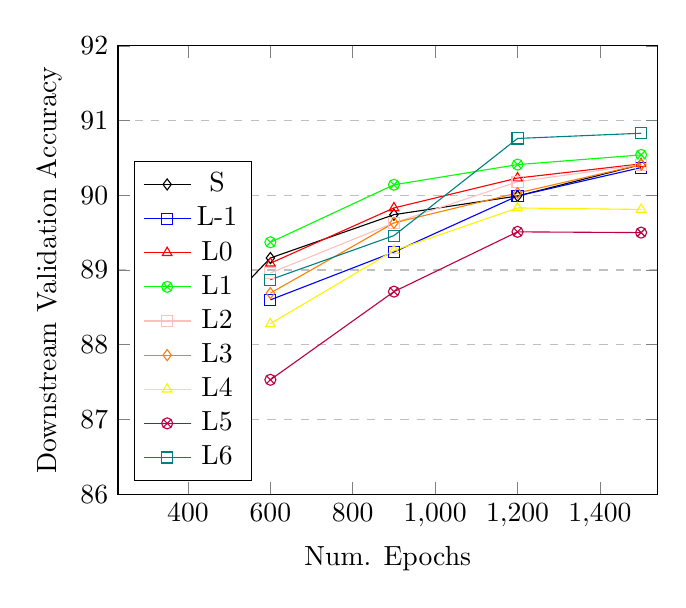
\begin{tikzpicture}
\begin{axis}[
    %title={Temperature dependence of CuSO\(_4\cdot\)5H\(_2\)O solubility},
    % width=0.8\textwidth,
    % height=0.5\textwidth,
    xlabel={Num. Epochs},
    ylabel={Downstream Validation Accuracy},
    xmin=230, xmax=1540,
    ymin=86, ymax=92,
    xtick={200,400,600,800,1000,1200,1400}, %,11,12,13},
    ytick={86,87,88,89,90,91,92},
    %ytick={0,0.2,0.4,0.6,0.8,1.0}, %,0.6,0.7,0.8,0.9,1.0},
    legend pos=south west,
    ymajorgrids=true,
    grid style=dashed,
]
\addplot[
    color=black,
    mark=diamond,
    ]
    coordinates {
    (300,87.43000030517578)(600,89.15999603271484)(900,89.73999786376953)(1200,89.98999786376953)(1500,90.40999603271484)
    };
    \addlegendentry{S}
\addplot[
    color=blue,
    mark=square,
    ]
    coordinates {
    (600,88.5999984741211)(900,89.23999786376953)(1200,89.98999786376953)(1500,90.3699951171875)
    };
    \addlegendentry{L-1}
\addplot[
    color=red,
    mark=triangle,
    ]
    coordinates {
    (600,89.08999633789062)(900,89.82999420166016)(1200,90.22999572753906)(1500,90.41999816894531)
    };
    
    \addlegendentry{L0}
\addplot[
    color=green,
    mark=otimes,
    ]
    coordinates {
    (600,89.3699951171875)(900,90.13999938964844)(1200,90.40999603271484)(1500,90.54000091552734)
    };
    
    \addlegendentry{L1}
\addplot[
    color=pink,
    mark=square,
    ]
    coordinates {
    (600,88.95999908447266)(900,89.62999725341797)(1200,90.18000030517578)(1500,90.40999603271484)
    };
    
    \addlegendentry{L2}
\addplot[
    color=orange,
    mark=diamond,
    ]
    coordinates {
    (600,88.68999481201172)(900,89.62999725341797)(1200,90.02999877929688)(1500,90.40999603271484)
    };
    
    \addlegendentry{L3}
\addplot[
    color=yellow,
    mark=triangle,
    ]
    coordinates {
    (600,88.27999877929688)(900,89.25999450683594)(1200,89.82999420166016)(1500,89.80999755859375)
    };
    
    \addlegendentry{L4}
\addplot[
    color=purple,
    mark=otimes,
    ]
    coordinates {
    (600,87.52999877929688)(900,88.70999908447266)(1200,89.50999450683594)(1500,89.5)
    };
    
    \addlegendentry{L5}
\addplot[
    color=teal,
    mark=square,
    ]
    coordinates {
    (600,88.8699951171875)(900,89.45999908447266)(1200,90.75999450683594)(1500,90.82999420166016)
    };
    \addlegendentry{L6}

\end{axis}
\end{tikzpicture}

}
%\vspace{-.1in}
\caption{Without stop-gradient}
\label{fig:trainble-cifar10-cifar10}
\end{subfigure}
\caption{Cifar10. Comparing sampling 50\% and applying 50\% dropout, with or without stop-gradient.}
\label{fig:cifar10-with-sg-without-sg-epochs}
\end{figure}

\begin{figure}
\begin{subfigure}{.49\columnwidth}
  \centering
  \resizebox{1.0\columnwidth}{!}{
  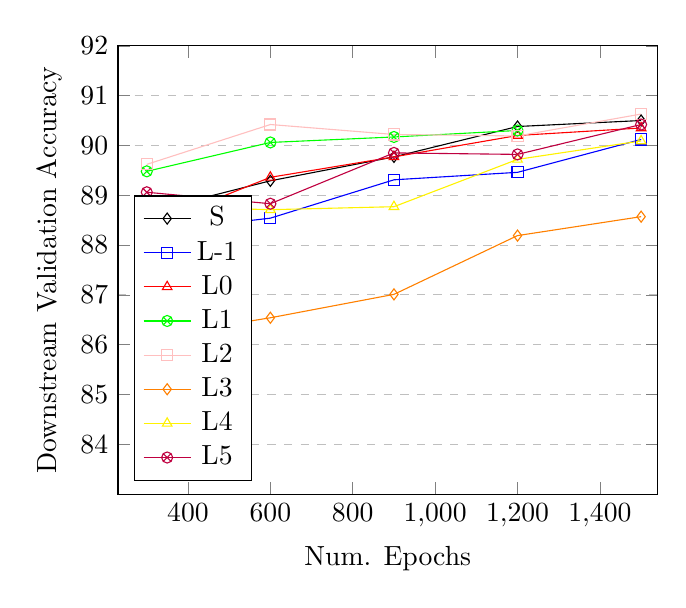
\begin{tikzpicture}
\begin{axis}[
    %title={Temperature dependence of CuSO\(_4\cdot\)5H\(_2\)O solubility},
    % width=0.8\textwidth,
    % height=0.5\textwidth,
    xlabel={Num. Epochs},
    ylabel={Downstream Validation Accuracy},
    xmin=230, xmax=1540,
    ymin=83, ymax=92,
    xtick={200,400,600,800,1000,1200,1400}, %,11,12,13},
    ytick={84,85,86,87,88,89,90,91,92},
    %ytick={0,0.2,0.4,0.6,0.8,1.0}, %,0.6,0.7,0.8,0.9,1.0},
    legend pos=south west,
    ymajorgrids=true,
    grid style=dashed,
]
\addplot[
    color=black,
    mark=diamond,
    ]
    coordinates {
    (300,88.65999603271484)(600,89.29000091552734)(900,89.7699966430664)(1200,90.37999725341797)(1500,90.5)
    };
    \addlegendentry{S}

\addplot[
    color=blue,
    mark=square,
    ]
    coordinates {
    (300,88.25)(600,88.54000091552734)(900,89.30999755859375)(1200,89.45999908447266)(1500,90.1199951171875)
    %(600,88.5999984741211)(900,89.23999786376953)(1200,89.98999786376953)(1500,90.3699951171875)
    };
    \addlegendentry{L-1}
\addplot[
    color=red,
    mark=triangle,
    ]
    coordinates {
    (300,88.3699951171875)(600,89.36000061035156)(900,89.7699966430664)(1200,90.19999694824219)(1500,90.3499984741211)
    };
    \addlegendentry{L0}
    
\addplot[
    color=green,
    mark=otimes,
    ]
    coordinates {
    (300,89.47999572753906)(600,90.05999755859375)(900,90.16999816894531)(1200,90.29999542236328)
    };
    
    \addlegendentry{L1}
\addplot[
    color=pink,
    mark=square,
    ]
    coordinates {
    (300,89.6199951171875)(600,90.41999816894531)(900,90.22000122070312)(1200,90.18999481201172)(1500,90.62999725341797)
    };
    
    \addlegendentry{L2}
\addplot[
    color=orange,
    mark=diamond,
    ]
    coordinates {
    (300,86.13999938964844)(600,86.54000091552734)(900,87.00999450683594)(1200,88.18999481201172)(1500,88.56999969482422)
    };
    \addlegendentry{L3}
    
\addplot[
    color=yellow,
    mark=triangle,
    ]
    coordinates {
    (300,88.77999877929688)(600,88.70999908447266)(900,88.7699966430664)(1200,89.72000122070312)(1500,90.08999633789062)
    };
    
    \addlegendentry{L4}
\addplot[
    color=purple,
    mark=otimes,
    ]
    coordinates {
    (300,89.05999755859375)(600,88.82999420166016)(900,89.8499984741211)(1200,89.81999969482422)(1500,90.41999816894531)
    };
    
    \addlegendentry{L5}
% \addplot[
%     color=teal,
%     mark=square,
%     ]
%     coordinates {
%     (300,86.8699951171875)(600,88.31999969482422)(900,89.6500015258789)(1200,90.31999969482422)(1500,91.32999420166016)
%     };
%     \addlegendentry{L6}

\end{axis}
\end{tikzpicture}
}
%\caption{Freeze Continue Cifar100-Cifar100}
\caption{Freeze layers before Deep Augmentation}
\label{fig:freeze-continue-cifar10-cifar10}
\end{subfigure}%
\hspace{0.005\columnwidth}
\begin{subfigure}{.49\columnwidth}
  \resizebox{1.0\columnwidth}{!}{
  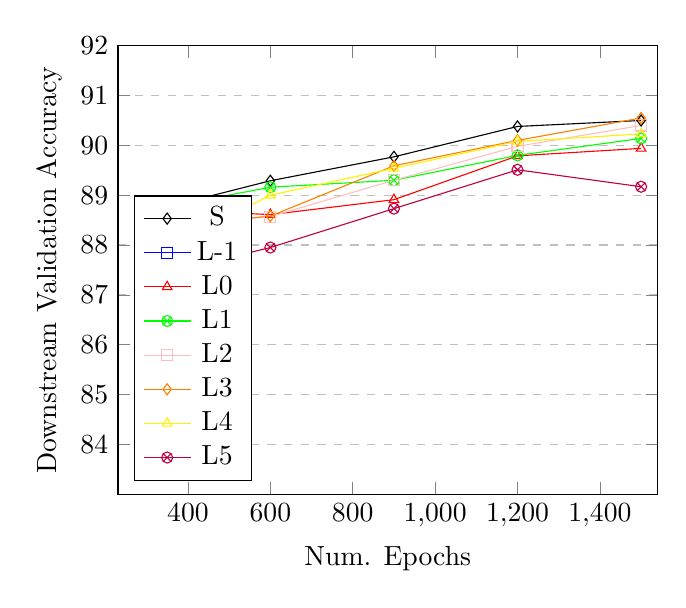
\begin{tikzpicture}
\begin{axis}[
    %title={Temperature dependence of CuSO\(_4\cdot\)5H\(_2\)O solubility},
    % width=0.8\textwidth,
    % height=0.5\textwidth,
    xlabel={Num. Epochs},
    ylabel={Downstream Validation Accuracy},
    xmin=230, xmax=1540,
    ymin=83, ymax=92,
    xtick={200,400,600,800,1000,1200,1400}, %,11,12,13},
    ytick={84,85,86,87,88,89,90,91,92},
    %ytick={0,0.2,0.4,0.6,0.8,1.0}, %,0.6,0.7,0.8,0.9,1.0},
    legend pos=south west,
    ymajorgrids=true,
    grid style=dashed,
]
\addplot[
    color=black,
    mark=diamond,
    ]
    coordinates {
    (300,88.65999603271484)(600,89.29000091552734)(900,89.7699966430664)(1200,90.37999725341797)(1500,90.5)
    };
    \addlegendentry{S}

\addplot[
    color=blue,
    mark=square,
    ]
    coordinates {(0,0)
    % (300,88.25)(600,88.54000091552734)(900,89.30999755859375)(1200,89.45999908447266)(1500,90.1199951171875)
    %(600,88.5999984741211)(900,89.23999786376953)(1200,89.98999786376953)(1500,90.3699951171875)
    };
    \addlegendentry{L-1}
\addplot[
    color=red,
    mark=triangle,
    ]
    coordinates {
    (300,88.72999572753906)(600,88.61000061035156)(900,88.90999603271484)(1200,89.79000091552734)(1500,89.93999481201172)
    };
    \addlegendentry{L0}
    
\addplot[
    color=green,
    mark=otimes,
    ]
    coordinates {
    (300,88.68999481201172)(600,89.15999603271484)(900,89.29999542236328)(1200,89.79999542236328)(1500,90.13999938964844)
    };
    
    \addlegendentry{L1}
\addplot[
    color=pink,
    mark=square,
    ]
    coordinates {
    (300,88.40999603271484)(600,88.56999969482422)(900,89.29999542236328)(1200,89.97999572753906)(1500,90.4000015258789)
    };
    
    \addlegendentry{L2}
\addplot[
    color=orange,
    mark=diamond,
    ]
    coordinates {
    (300,88.31999969482422)(600,88.57999420166016)(900,89.58999633789062)(1200,90.0999984741211)(1500,90.54999542236328)
    };
    \addlegendentry{L3}
    
    
\addplot[
    color=yellow,
    mark=triangle,
    ]
    coordinates {
    (300,87.72999572753906)(600,89.0)(900,89.54000091552734)(1200,90.07999420166016)(1500,90.22999572753906)
    };
    
    \addlegendentry{L4}
\addplot[
    color=purple,
    mark=otimes,
    ]
    coordinates {
    (300,87.33999633789062)(600,87.94999694824219)(900,88.72999572753906)(1200,89.50999450683594)(1500,89.16999816894531)
    };
    
    
    \addlegendentry{L5}
% \addplot[
%     color=teal,
%     mark=square,
%     ]
%     coordinates {
%     (300,86.8699951171875)(600,88.31999969482422)(900,89.6500015258789)(1200,90.31999969482422)(1500,91.32999420166016)
%     };
%     \addlegendentry{L6}

\end{axis}
\end{tikzpicture}
}
%\vspace{-.1in}
%\caption{Continue Freeze Reverse Cifar100-Cifar100}
\caption{Freeze layers after Deep Augmentation}
\label{fig:freeze-reverse-continue-cifar10-cifar10}
\end{subfigure}
\caption{Cifar10. Comparing freezing layers before or after Deep Augmentation with stop-gradient initialized with pre-trained SimCLR model.}
\label{fig:cifar10-freezingbeforeafter-epochs}
\end{figure}


\begin{figure}
\begin{subfigure}{.49\columnwidth}
  \centering
  \resizebox{1.0\columnwidth}{!}{
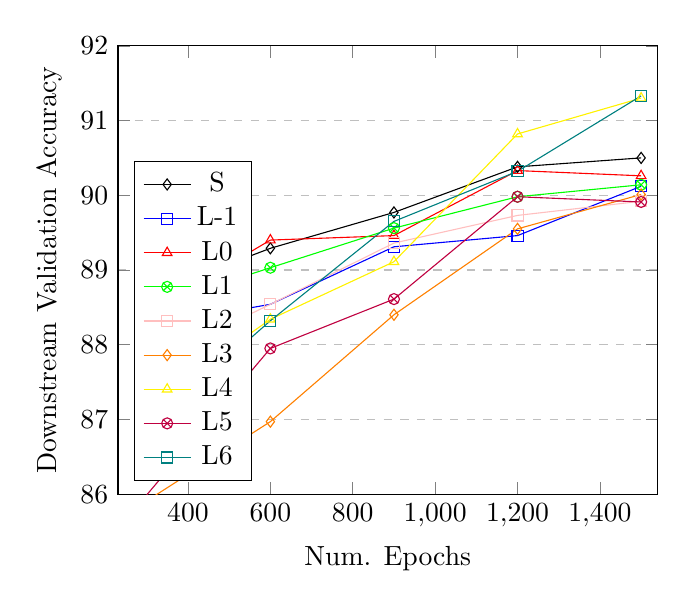
\begin{tikzpicture}
\begin{axis}[
    %title={Temperature dependence of CuSO\(_4\cdot\)5H\(_2\)O solubility},
    % width=0.8\textwidth,
    % height=0.5\textwidth,
    xlabel={Num. Epochs},
    ylabel={Downstream Validation Accuracy},
    xmin=230, xmax=1540,
    ymin=86, ymax=92,
    xtick={200,400,600,800,1000,1200,1400}, %,11,12,13},
    ytick={86,87,88,89,90,91,92},
    %ytick={0,0.2,0.4,0.6,0.8,1.0}, %,0.6,0.7,0.8,0.9,1.0},
    legend pos=south west,
    ymajorgrids=true,
    grid style=dashed,
]
\addplot[
    color=black,
    mark=diamond,
    ]
    coordinates {
    (300,88.65999603271484)(600,89.29000091552734)(900,89.7699966430664)(1200,90.37999725341797)(1500,90.5)
    };
    \addlegendentry{S}

\addplot[
    color=blue,
    mark=square,
    ]
    coordinates {
    (300,88.25)(600,88.54000091552734)(900,89.30999755859375)(1200,89.45999908447266)(1500,90.1199951171875)
    %(600,88.5999984741211)(900,89.23999786376953)(1200,89.98999786376953)(1500,90.3699951171875)
    };
    \addlegendentry{L-1}
    
\addplot[
    color=red,
    mark=triangle,
    ]
    coordinates {
    (300,88.41999816894531)(600,89.4000015258789)(900,89.45999908447266)(1200,90.32999420166016)(1500,90.25999450683594)
    
    
    };
    \addlegendentry{L0}
\addplot[
    color=green,
    mark=otimes,
    ]
    coordinates {
    (300,88.48999786376953)(600,89.02999877929688)(900,89.55999755859375)(1200,89.97999572753906)(1500,90.13999938964844)
    
    };
    \addlegendentry{L1}
\addplot[
    color=pink,
    mark=square,
    ]
    coordinates {
    (300,87.73999786376953)(600,88.54000091552734)(900,89.36000061035156)(1200,89.72999572753906)(1500,89.91999816894531)
    
    };
    \addlegendentry{L2}
\addplot[
    color=orange,
    mark=diamond,
    ]
    coordinates {
    (300,85.90999603271484)(600,86.97000122070312)(900,88.4000015258789)(1200,89.54999542236328)(1500,90.00999450683594)
    
    };
    \addlegendentry{L3}
\addplot[
    color=yellow,
    mark=triangle,
    ]
    coordinates {
    (300,87.16999816894531)(600,88.33999633789062)(900,89.11000061035156)(1200,90.81999969482422)(1500,91.29999542236328)
    
    };
    \addlegendentry{L4}
\addplot[
    color=purple,
    mark=otimes,
    ]
    coordinates {
    (300,85.98999786376953)(600,87.94999694824219)(900,88.61000061035156)(1200,89.97999572753906)(1500,89.90999603271484)
    
    };
    \addlegendentry{L5}
\addplot[
    color=teal,
    mark=square,
    ]
    coordinates {
    (300,86.8699951171875)(600,88.31999969482422)(900,89.6500015258789)(1200,90.31999969482422)(1500,91.32999420166016)
    % (300,88.04999542236328)(600,89.32999420166016)(900,90.19999694824219)(1200,90.45999908447266)(1500,91.32999420166016)
    
    };
    \addlegendentry{L6}

\end{axis}
\end{tikzpicture}
}
\caption{With stop-gradient.}
\label{fig:continue-cifar10-cifar10}
\end{subfigure}%
\hspace{0.005\columnwidth}
\begin{subfigure}{.49\columnwidth}
  \centering
  \resizebox{1.0\columnwidth}{!}{
\centering
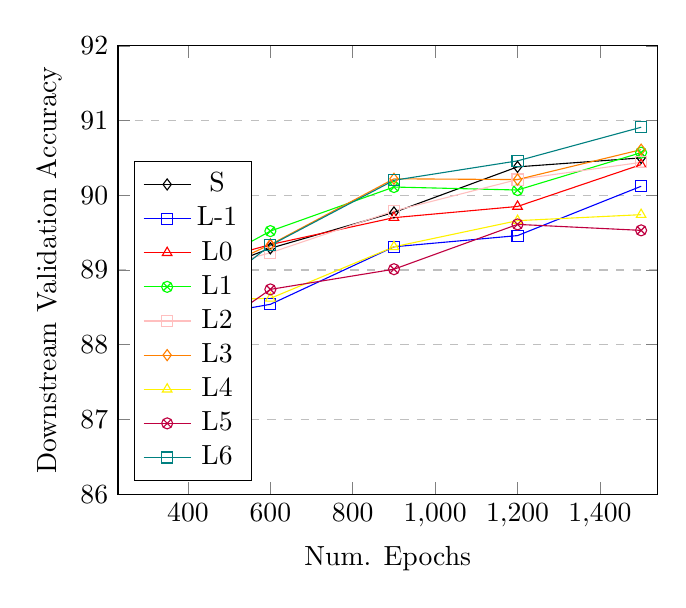
\begin{tikzpicture}
\begin{axis}[
    %title={Temperature dependence of CuSO\(_4\cdot\)5H\(_2\)O solubility},
    % width=0.8\textwidth,
    % height=0.5\textwidth,
    xlabel={Num. Epochs},
    ylabel={Downstream Validation Accuracy},
    xmin=230, xmax=1540,
    ymin=86, ymax=92,
    xtick={200,400,600,800,1000,1200,1400}, %,11,12,13},
    ytick={86,87,88,89,90,91,92},
    %ytick={0,0.2,0.4,0.6,0.8,1.0}, %,0.6,0.7,0.8,0.9,1.0},
    legend pos=south west,
    ymajorgrids=true,
    grid style=dashed,
]
\addplot[
    color=black,
    mark=diamond,
    ]
    coordinates {
    (300,88.65999603271484)(600,89.29000091552734)(900,89.7699966430664)(1200,90.37999725341797)(1500,90.5)
    };
    \addlegendentry{S}

\addplot[
    color=blue,
    mark=square,
    ]
    coordinates {
    (300,88.25)(600,88.54000091552734)(900,89.30999755859375)(1200,89.45999908447266)(1500,90.1199951171875)
    };
    \addlegendentry{L-1}
\addplot[
    color=red,
    mark=triangle,
    ]
    coordinates {
    (300,88.87999725341797)(600,89.33999633789062)(900,89.69999694824219)(1200,89.8499984741211)(1500,90.40999603271484)
    
    };
    \addlegendentry{L0}
\addplot[
    color=green,
    mark=otimes,
    ]
    coordinates {
    (300,88.6199951171875)(600,89.5199966430664)(900,90.11000061035156)(1200,90.06999969482422)(1500,90.56999969482422)
    
    };
    \addlegendentry{L1}
\addplot[
    color=pink,
    mark=square,
    ]
    coordinates {
    (300,88.77999877929688)(600,89.22999572753906)(900,89.79000091552734)(1200,90.20999908447266)(1500,90.43999481201172)
    
    };
    \addlegendentry{L2}
\addplot[
    color=orange,
    mark=diamond,
    ]
    coordinates {
    (300,88.56999969482422)(600,89.33999633789062)(900,90.22000122070312)(1200,90.20999908447266)(1500,90.61000061035156)
    
    };
    \addlegendentry{L3}
\addplot[
    color=yellow,
    mark=triangle,
    ]
    coordinates {
    (300,88.57999420166016)(600,88.6199951171875)(900,89.30999755859375)(1200,89.65999603271484)(1500,89.73999786376953)
    
    };
    \addlegendentry{L4}
\addplot[
    color=purple,
    mark=otimes,
    ]
    coordinates {
    (300,87.58999633789062)(600,88.73999786376953)(900,89.00999450683594)(1200,89.61000061035156)(1500,89.52999877929688)
    
    };
    \addlegendentry{L5}
\addplot[
    color=teal,
    mark=square,
    ]
    coordinates {
    (300,88.04999542236328)(600,89.32999420166016)(900,90.19999694824219)(1200,90.45999908447266)(1500,90.90999603271484)
    % (300,86.8699951171875)(600,88.31999969482422)(900,89.6500015258789)(1200,90.31999969482422)(1500,91.32999420166016)
    };
    \addlegendentry{L6}

\end{axis}
\end{tikzpicture}
%\vspace{-.1in}
}
\caption{Without stop-gradient.}
\label{fig:continue-trainable-cifar10-cifar10}
\end{subfigure}
\caption{Cifar10. 50\% sampling, 50\% dropout, with and without stop-gradient, and initialized with pre-trained SimCLR model.}
\label{fig:continue-cifar10-epochs}
\end{figure}



\begin{figure}
\begin{subfigure}{.49\columnwidth}
\resizebox{\columnwidth}{!}{%
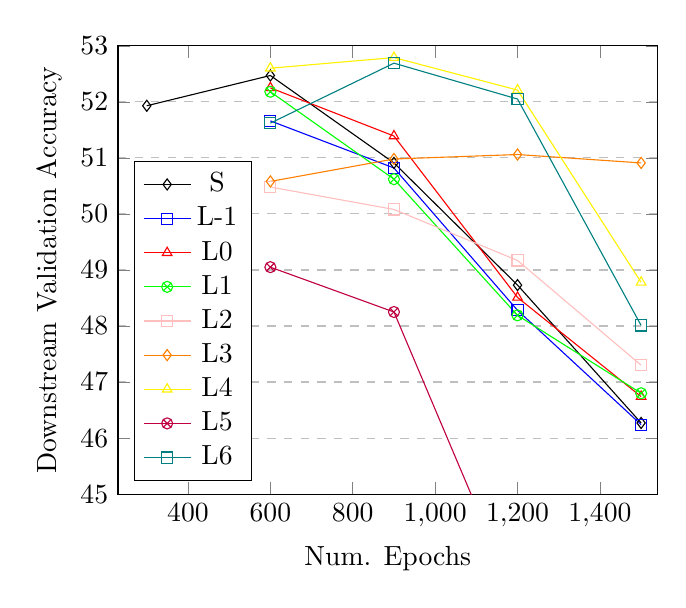
\begin{tikzpicture}
\begin{axis}[
    %title={Temperature dependence of CuSO\(_4\cdot\)5H\(_2\)O solubility},
    % width=0.8\textwidth,
    % height=0.5\textwidth,
    xlabel={Num. Epochs},
    ylabel={Downstream Validation Accuracy},
    xmin=230, xmax=1540,
    ymin=45, ymax=53,
    xtick={200,400,600,800,1000,1200,1400}, %,11,12,13},
    ytick={43,44,45,46,47,48,49,50,51,52,53,54},
    %ytick={0,0.2,0.4,0.6,0.8,1.0}, %,0.6,0.7,0.8,0.9,1.0},
    legend pos=south west,
    ymajorgrids=true,
    grid style=dashed,
]
\addplot[
    color=black,
    mark=diamond,
    ]
    coordinates {
    (300,51.93000030517578)(600,52.46999740600586)(900,50.90999984741211)(1200,48.72999954223633)(1500,46.27000045776367)
    };
    \addlegendentry{S}

\addplot[
    color=blue,
    mark=square,
    ]
    coordinates {
    (600,51.65999984741211)(900,50.81999969482422)(1200,48.279998779296875)(1500,46.23999786376953)
    };
    \addlegendentry{L-1}
\addplot[
    color=red,
    mark=triangle,
    ]
    coordinates {
    (600,52.25)(900,51.38999938964844)(1200,48.5099983215332)(1500,46.73999786376953)
    };
    
    \addlegendentry{L0}
\addplot[
    color=green,
    mark=otimes,
    ]
    coordinates {
   (600,52.18000030517578)(900,50.619998931884766)(1200,48.189998626708984)(1500,46.79999923706055)
    };
    
    \addlegendentry{L1}
\addplot[
    color=pink,
    mark=square,
    ]
    coordinates {
    (600,50.47999954223633)(900,50.07999801635742)(1200,49.16999816894531)(1500,47.29999923706055)
    };
    
    \addlegendentry{L2}
\addplot[
    color=orange,
    mark=diamond,
    ]
    coordinates {
    (600,50.57999801635742)(900,50.97999954223633)(1200,51.05999755859375)(1500,50.90999984741211)
    };
    
    \addlegendentry{L3}
\addplot[
    color=yellow,
    mark=triangle,
    ]
    coordinates {
   (600,52.599998474121094)(900,52.78999710083008)(1200,52.209999084472656)(1500,48.779998779296875)
    };
    
    \addlegendentry{L4}
\addplot[
    color=purple,
    mark=otimes,
    ]
    coordinates {
    (600,49.04999923706055)(900,48.25)(1200,43.03999710083008)(1500,35.84000015258789)
    };
    
    \addlegendentry{L5}
\addplot[
    color=teal,
    mark=square,
    ]
    coordinates {
    (600,51.619998931884766)(900,52.689998626708984)(1200,52.04999923706055)(1500,48.0099983215332)
    };
    
    \addlegendentry{L6}

\end{axis}
\end{tikzpicture}

}
%\vspace{-.1in}
\caption{With stop-gradient.}
\label{fig:cifar10-cifar100-stop}
\end{subfigure}%
\hspace{0.005\columnwidth}
\begin{subfigure}{.49\columnwidth}
\centering
\resizebox{\columnwidth}{!}{%
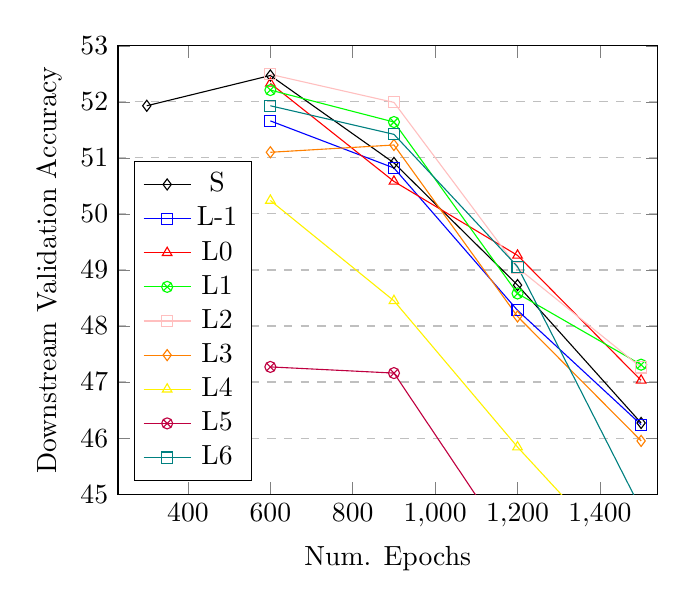
\begin{tikzpicture}
\begin{axis}[
    %title={Temperature dependence of CuSO\(_4\cdot\)5H\(_2\)O solubility},
    % width=0.8\textwidth,
    % height=0.5\textwidth,
    xlabel={Num. Epochs},
    ylabel={Downstream Validation Accuracy},
    xmin=230, xmax=1540,
    ymin=45, ymax=53,
    xtick={200,400,600,800,1000,1200,1400}, %,11,12,13},
    ytick={43,44,45,46,47,48,49,50,51,52,53,54},
    %ytick={0,0.2,0.4,0.6,0.8,1.0}, %,0.6,0.7,0.8,0.9,1.0},
    legend pos=south west,
    ymajorgrids=true,
    grid style=dashed,
]
\addplot[
    color=black,
    mark=diamond,
    ]
    coordinates {
    (300,51.93000030517578)(600,52.46999740600586)(900,50.90999984741211)(1200,48.72999954223633)(1500,46.27000045776367)
    };
    \addlegendentry{S}
\addplot[
    color=blue,
    mark=square,
    ]
    coordinates {
    (600,51.65999984741211)(900,50.81999969482422)(1200,48.279998779296875)(1500,46.23999786376953)
    };
    \addlegendentry{L-1}
    
\addplot[
    color=red,
    mark=triangle,
    ]
    coordinates {
    (600,52.32999801635742)(900,50.57999801635742)(1200,49.2599983215332)(1500,47.029998779296875)
    };
    \addlegendentry{L0}
    
\addplot[
    color=green,
    mark=otimes,
    ]
    coordinates {
    (600,52.209999084472656)(900,51.63999938964844)(1200,48.57999801635742)(1500,47.30999755859375)
    };
    
    \addlegendentry{L1}
\addplot[
    color=pink,
    mark=square,
    ]
    coordinates {
    (600,52.48999786376953)(900,51.98999786376953)(1200,49.03999710083008)(1500,47.2599983215332)
    };
    
    \addlegendentry{L2}
\addplot[
    color=orange,
    mark=diamond,
    ]
    coordinates {
    (600,51.099998474121094)(900,51.22999954223633)(1200,48.16999816894531)(1500,45.94999694824219)
    };
    
    \addlegendentry{L3}
\addplot[
    color=yellow,
    mark=triangle,
    ]
    coordinates {
    (600,50.23999786376953)(900,48.44999694824219)(1200,45.84000015258789)(1500,43.45000076293945)
    };
    
    \addlegendentry{L4}
\addplot[
    color=purple,
    mark=otimes,
    ]
    coordinates {
    (600,47.27000045776367)(900,47.15999984741211)(1200,43.869998931884766)(1500,41.06999969482422)
    };
    \addlegendentry{L5}
    
\addplot[
    color=teal,
    mark=square,
    ]
    coordinates {
    (600,51.93000030517578)(900,51.41999816894531)(1200,49.05999755859375)(1500,44.72999954223633)
    };
    \addlegendentry{L6}

\end{axis}
\end{tikzpicture}


}
\caption{Without stop-gradient}
\label{fig:cifar10-cifar100-train}
\end{subfigure}
\caption{SimCLR and Deep Augmenation with and without stop-gradient pre-trained on Cifar10 and finetuned on Cifar100, for different checkpoints during training. Observe the overfitting behavior.}
\label{fig:cifar10-cifar100-epochs}
\end{figure}

\subsection{Freezing Layers}
\label{appendix:freezing-layers}

Further adding to the discussion about freezing layers. We see that Deep Augmentation with freezing layers and initialized to SimCLR-model, works better for earlier layers than for later layers. Especially in Figure \ref{fig:freeze-continue-cifar100-cifar100} and \ref{fig:cifar10-freezingbeforeafter-epochs}, we see that earlier layers outperform SimCLR earlier in the training. This suggests that incrementally freezing layers, and adding Deep Augmentation at the next layer, might help improve performance and speed up training.

% The Figures in Sections \ref{sec:cifar100-across-epochs} and \ref{sec:cifar10-across-epochs}, provides a more nuanced depiction of the performance of Deep Augmentation at different layers as well as SimCLR.  



\subsection{Cifar100 Miscellaneous Experiments}

We include some preliminary results on different aspects of Deep Augmentation that deserve further investigation. 

In Figure \ref{fig:cifar100-cifar100-onesided}, we include results of Deep Augmentation with stop-gradient where each pair consists of one sample that has only input-data augmentation and another sample that has input-data and higher-layer augmentation. I.e. we remove all the higher-to-higher and lower-to-lower pairs. We see that for Layer 4 and 6 the performance does not change substantially, but for Layer 3 performance degrades substantially.

In Figure \ref{fig:cifar100-cifar100-onesided-trainable}, we include results of Deep Augmentation without stop-gradient where each pair consists of one sample that has only input-data augmentation and another sample that has input-data and higher-layer augmentation. I.e. we remove all the higher-to-higher and lower-to-lower pairs. We see that for the layers involved performance does not change substantially.

This suggests that lower-to-higher pairs are sufficient to make Deep Augmentation successful, but that certain layers are greatly helped by also including other lower-to-lower or higher-to-higher pairs.

In Figure \ref{fig:cifar100-cifar100-random-freeze}, we include results of Deep Augmentation with stop-gradient and freezing layers before, but initialized with random weights instead of initialized with a pre-trained SimCLR model. We note that several layers are severely hurt by this compared to the SimCLR pre-trained model initialization. 

In Figure \ref{fig:cifar100-cifar100-random-dropout-freeze}, we include results of Deep Augmentation with stop-gradient and freezing layers before, but initialized with a model pre-trained with SimCLR and 20\% dropout across all layers. We wanted to see if a model trained with high dropout everywhere was more helpful as a starting point for Deep Augmentation. Future work may investigate ways to optimally train a NN so that dropout serves as a useful higher transformation. 



\begin{figure}
\begin{subfigure}{.49\columnwidth}
\resizebox{\columnwidth}{!}{%
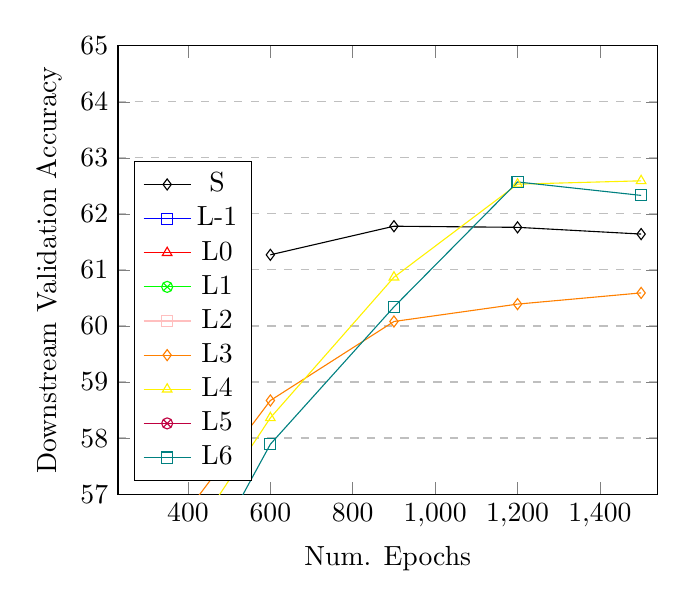
\begin{tikzpicture}
\begin{axis}[
    %title={Temperature dependence of CuSO\(_4\cdot\)5H\(_2\)O solubility},
    % width=0.8\textwidth,
    % height=0.5\textwidth,
    xlabel={Num. Epochs},
    ylabel={Downstream Validation Accuracy},
    xmin=230, xmax=1540,
    ymin=57, ymax=65,
    xtick={200,400,600,800,1000,1200,1400}, %,11,12,13},
    ytick={57, 58, 59, 60, 61, 62, 63, 64, 65},
    %ytick={0,0.2,0.4,0.6,0.8,1.0}, %,0.6,0.7,0.8,0.9,1.0},
    legend pos=south west,
    ymajorgrids=true,
    grid style=dashed,
]
\addplot[
    color=black,
    mark=diamond,
    ]
    coordinates {
    (600,61.27)(900,61.78)(1200,61.76)(1500,61.64)
    };
    \addlegendentry{S}

\addplot[
    color=blue,
    mark=square,
    ]
    coordinates {
    (0,0)
    };
    \addlegendentry{L-1}
\addplot[
    color=red,
    mark=triangle,
    ]
    coordinates {
    (0,0)
    };
    \addlegendentry{L0}
\addplot[
    color=green,
    mark=otimes,
    ]
    coordinates {
    (0,0)
    };
    \addlegendentry{L1}
\addplot[
    color=pink,
    mark=square,
    ]
    coordinates {
    (0,0)
    };
    \addlegendentry{L2}
\addplot[
    color=orange,
    mark=diamond,
    ]
    coordinates {
    (300,55.73999786376953)(600,58.66999816894531)(900,60.07999801635742)(1200,60.38999938964844)(1500,60.59000015258789)
    };
    \addlegendentry{L3}
\addplot[
    color=yellow,
    mark=triangle,
    ]
    coordinates {
    (300,55.029998779296875)(600,58.3599967956543)(900,60.869998931884766)(1200,62.529998779296875)(1500,62.59000015258789)
    };
    \addlegendentry{L4}
\addplot[
    color=purple,
    mark=otimes,
    ]
    coordinates {
    (300,43.029998779296875)(600,48.04999923706055)(900,49.96999740600586)(1200,50.14999771118164)(1500,52.02000045776367)
    };
    \addlegendentry{L5}
\addplot[
    color=teal,
    mark=square,
    ]
    coordinates {
    (300,53.84000015258789)(600,57.88999938964844)(900,60.34000015258789)(1200,62.56999969482422)(1500,62.32999801635742)
    };
    \addlegendentry{L6}

\end{axis}
\end{tikzpicture}

}
%\vspace{-.1in}
\caption{Random initialization.}
%\label{fig:cifar100-cifar100-onesided}
\end{subfigure}%
\hspace{0.005\columnwidth}
\begin{subfigure}{.49\columnwidth}
\centering
\resizebox{\columnwidth}{!}{%
\begin{tikzpicture}
\begin{axis}[
    %title={Temperature dependence of CuSO\(_4\cdot\)5H\(_2\)O solubility},
    % width=0.8\textwidth,
    % height=0.5\textwidth,
    xlabel={Num. Epochs},
    ylabel={Downstream Validation Accuracy},
    xmin=230, xmax=1540,
    ymin=57, ymax=65,
    xtick={200,400,600,800,1000,1200,1400}, %,11,12,13},
    ytick={57, 58, 59, 60, 61, 62, 63, 64, 65},
    %ytick={0,0.2,0.4,0.6,0.8,1.0}, %,0.6,0.7,0.8,0.9,1.0},
    legend pos=south west,
    ymajorgrids=true,
    grid style=dashed,
]
\addplot[
    color=black,
    mark=diamond,
    ]
    coordinates {
    (300,62.79999923706055)(600,62.5)(900,62.87999725341797)(1200,62.28999710083008)(1500,61.91999816894531)
    };
    \addlegendentry{S}

\addplot[
    color=blue,
    mark=square,
    ]
    coordinates {
    (0,0)
    };
    \addlegendentry{L-1}
\addplot[
    color=red,
    mark=triangle,
    ]
    coordinates {
    (0,0)
    };
    \addlegendentry{L0}
\addplot[
    color=green,
    mark=otimes,
    ]
    coordinates {
    (0,0)
    };
    \addlegendentry{L1}
\addplot[
    color=pink,
    mark=square,
    ]
    coordinates {
    (0,0)
    };
    \addlegendentry{L2}
\addplot[
    color=orange,
    mark=diamond,
    ]
    coordinates {
    (300,59.0)(600,59.65999984741211)(900,60.03999710083008)(1200,61.37999725341797)(1500,60.7599983215332)
    };
    \addlegendentry{L3}
\addplot[
    color=yellow,
    mark=triangle,
    ]
    coordinates {
    (300,60.2599983215332)(600,61.22999954223633)(900,62.689998626708984)(1200,63.94999694824219)(1500,63.349998474121094)
    };
    \addlegendentry{L4}
\addplot[
    color=purple,
    mark=otimes,
    ]
    coordinates {
    (600,55.90999984741211)(900,56.30999755859375)(1200,56.09000015258789)(1500,53.87999725341797)
    };
    \addlegendentry{L5}
\addplot[
    color=teal,
    mark=square,
    ]
    coordinates {
    (300,58.41999816894531)(600,60.5099983215332)(900,61.709999084472656)(1200,64.04999542236328)(1500,64.22999572753906)
    };
    \addlegendentry{L6}

\end{axis}
\end{tikzpicture}


}
\caption{SimCLR initialization}
\label{fig:cifar100-cifar100-one-sided-continue}
\end{subfigure}
\caption{Deep Augmentation with stop-gradient, only lower-to-higher augmentation pairs. }
\label{fig:cifar100-cifar100-onesided}
\end{figure}


\begin{figure}
\centering
\begin{subfigure}{.49\columnwidth}
\resizebox{\columnwidth}{!}{%
\begin{tikzpicture}
\begin{axis}[
    %title={Temperature dependence of CuSO\(_4\cdot\)5H\(_2\)O solubility},
    % width=0.8\textwidth,
    % height=0.5\textwidth,
    xlabel={Num. Epochs},
    ylabel={Downstream Validation Accuracy},
    xmin=230, xmax=1540,
    ymin=57, ymax=65,
    xtick={200,400,600,800,1000,1200,1400}, %,11,12,13},
    ytick={57, 58, 59, 60, 61, 62, 63, 64, 65},
    %ytick={0,0.2,0.4,0.6,0.8,1.0}, %,0.6,0.7,0.8,0.9,1.0},
    legend pos=south west,
    ymajorgrids=true,
    grid style=dashed,
]
\addplot[
    color=black,
    mark=diamond,
    ]
    coordinates {
    (600,61.27)(900,61.78)(1200,61.76)(1500,61.64)
    };
    \addlegendentry{S}

\addplot[
    color=blue,
    mark=square,
    ]
    coordinates {
    (0,0)
    };
    \addlegendentry{L-1}
\addplot[
    color=red,
    mark=triangle,
    ]
    coordinates {
    (0,0)
    };
    \addlegendentry{L0}
\addplot[
    color=green,
    mark=otimes,
    ]
    coordinates {
    (0,0)
    };
    \addlegendentry{L1}
\addplot[
    color=pink,
    mark=square,
    ]
    coordinates {
    (0,0)
    };
    \addlegendentry{L2}
\addplot[
    color=orange,
    mark=diamond,
    ]
    coordinates {
    (300,58.709999084472656)(600,60.369998931884766)(900,61.55999755859375)(1200,60.8599967956543)(1500,60.849998474121094)
    };
    \addlegendentry{L3}
\addplot[
    color=yellow,
    mark=triangle,
    ]
    coordinates {
    (300,57.209999084472656)(600,59.2599983215332)(900,59.73999786376953)(1200,59.209999084472656)(1500,59.689998626708984)
    };
    \addlegendentry{L4}
\addplot[
    color=purple,
    mark=otimes,
    ]
    coordinates {
    (300,54.43000030517578)(600,56.84000015258789)(900,59.23999786376953)(1200,59.04999923706055)(1500,57.869998931884766)
    };
    \addlegendentry{L5}
\addplot[
    color=teal,
    mark=square,
    ]
    coordinates {
    (300,58.71999740600586)(600,60.94999694824219)(900,61.98999786376953)(1200,62.769996643066406)(1500,61.6099967956543)
    };
    \addlegendentry{L6}

\end{axis}
\end{tikzpicture}

}
%\vspace{-.1in}
\caption{Random initialization.}
%\label{fig:cifar100-cifar100-onesided-trainable}
\end{subfigure}%
\hspace{0.005\columnwidth}
% \begin{subfigure}{.49\columnwidth}
% \centering
% \resizebox{\columnwidth}{!}{%
% \begin{tikzpicture}
% \begin{axis}[
%     %title={Temperature dependence of CuSO\(_4\cdot\)5H\(_2\)O solubility},
%     % width=0.8\textwidth,
%     % height=0.5\textwidth,
%     xlabel={Num. Epochs},
%     ylabel={Downstream Validation Accuracy},
%     xmin=230, xmax=1540,
%     ymin=57, ymax=65,
%     xtick={200,400,600,800,1000,1200,1400}, %,11,12,13},
%     ytick={57, 58, 59, 60, 61, 62, 63, 64, 65},
%     %ytick={0,0.2,0.4,0.6,0.8,1.0}, %,0.6,0.7,0.8,0.9,1.0},
%     legend pos=south west,
%     ymajorgrids=true,
%     grid style=dashed,
% ]
% \addplot[
%     color=black,
%     mark=diamond,
%     ]
%     coordinates {
%     (300,62.79999923706055)(600,62.5)(900,62.87999725341797)(1200,62.28999710083008)(1500,61.91999816894531)
%     };
%     \addlegendentry{S}

% \addplot[
%     color=blue,
%     mark=square,
%     ]
%     coordinates {
%     (0,0)
%     };
%     \addlegendentry{L-1}
% \addplot[
%     color=red,
%     mark=triangle,
%     ]
%     coordinates {
%     (0,0)
%     };
%     \addlegendentry{L0}
% \addplot[
%     color=green,
%     mark=otimes,
%     ]
%     coordinates {
%     (0,0)
%     };
%     \addlegendentry{L1}
% \addplot[
%     color=pink,
%     mark=square,
%     ]
%     coordinates {
%     (0,0)
%     };
%     \addlegendentry{L2}
% \addplot[
%     color=orange,
%     mark=diamond,
%     ]
%     coordinates {
%     (300,59.0)(600,59.65999984741211)(900,60.03999710083008)(1200,61.37999725341797)(1500,60.7599983215332)
%     };
%     \addlegendentry{L3}
% \addplot[
%     color=yellow,
%     mark=triangle,
%     ]
%     coordinates {
%     (300,60.2599983215332)(600,61.22999954223633)(900,62.689998626708984)(1200,63.94999694824219)(1500,63.349998474121094)
%     };
%     \addlegendentry{L4}
% \addplot[
%     color=purple,
%     mark=otimes,
%     ]
%     coordinates {
%     (600,55.90999984741211)(900,56.30999755859375)(1200,56.09000015258789)(1500,53.87999725341797)
%     };
%     \addlegendentry{L5}
% \addplot[
%     color=teal,
%     mark=square,
%     ]
%     coordinates {
%     (300,58.41999816894531)(600,60.5099983215332)(900,61.709999084472656)(1200,64.04999542236328)(1500,64.22999572753906)
%     };
%     \addlegendentry{L6}

% \end{axis}
% \end{tikzpicture}


% }
% \caption{SimCLR initialization}
% \label{fig:cifar100-cifar100-one-sided-continue-trainable}
% \end{subfigure}
\caption{Deep Augmentation without stop-gradient, only lower-to-higher augmentation pairs. }
\label{fig:cifar100-cifar100-onesided-trainable}
\end{figure}



\begin{figure}
\centering
\begin{subfigure}{.49\columnwidth}
\resizebox{\columnwidth}{!}{%
\begin{tikzpicture}
\begin{axis}[
    %title={Temperature dependence of CuSO\(_4\cdot\)5H\(_2\)O solubility},
    % width=0.8\textwidth,
    % height=0.5\textwidth,
    xlabel={Num. Epochs},
    ylabel={Downstream Validation Accuracy},
    xmin=230, xmax=1540,
    ymin=35, ymax=65,
    xtick={200,400,600,800,1000,1200,1400}, %,11,12,13},
    ytick={40,50,60},
    %ytick={0,0.2,0.4,0.6,0.8,1.0}, %,0.6,0.7,0.8,0.9,1.0},
    legend pos=south west,
    ymajorgrids=true,
    grid style=dashed,
]
\addplot[
    color=black,
    mark=diamond,
    ]
    coordinates {
    (600,61.27)(900,61.78)(1200,61.76)(1500,61.64)
    };
    \addlegendentry{S}
\addplot[
    color=blue,
    mark=square,
    ]
    coordinates {
    (600,60.959999084472656)(900,62.39999771118164)(1200,61.12999725341797)(1500,61.43000030517578)
    };
    \addlegendentry{L-1}
\addplot[
    color=red,
    mark=triangle,
    ]
    coordinates {
    (300,58.89999771118164)(600,61.34000015258789)(900,62.69999694824219)(1200,61.40999984741211)(1500,61.56999969482422)
    };
    \addlegendentry{L0}
\addplot[
    color=green,
    mark=otimes,
    ]
    coordinates {
    (300,56.22999954223633)(600,58.209999084472656)(900,59.939998626708984)(1200,59.23999786376953)(1500,59.529998779296875)
    };
    \addlegendentry{L1}
\addplot[
    color=pink,
    mark=square,
    ]
    coordinates {
    (300,50.07999801635742)(600,51.529998779296875)(900,53.06999969482422)(1200,54.09000015258789)(1500,55.0099983215332)
    };
    \addlegendentry{L2}
\addplot[
    color=orange,
    mark=diamond,
    ]
    coordinates {
    (300,35.849998474121094)(600,36.599998474121094)(900,38.91999816894531)(1200,40.54999923706055)(1500,38.02000045776367)
    };
    \addlegendentry{L3}
\addplot[
    color=yellow,
    mark=triangle,
    ]
    coordinates {
    (300,36.66999816894531)(600,38.95000076293945)(900,39.81999969482422)(1200,41.91999816894531)(1500,43.96999740600586)
    };
    \addlegendentry{L4}
\addplot[
    color=purple,
    mark=otimes,
    ]
    coordinates {
    (300,35.529998779296875)(600,36.98999786376953)(900,37.80999755859375)(1200,39.869998931884766)(1500,41.18000030517578)
    };
    \addlegendentry{L5}


\end{axis}
\end{tikzpicture}

}
%\vspace{-.1in}
%\caption{Random initialization.}
%\label{fig:cifar100-cifar100-onesided-trainable}
\end{subfigure}%
\caption{Deep Augmentation with stop-gradient and random initialization, freeze layers before.}
\label{fig:cifar100-cifar100-random-freeze}
\end{figure}



\begin{figure}
\centering
\begin{subfigure}{.49\columnwidth}
\resizebox{\columnwidth}{!}{%
\begin{tikzpicture}
\begin{axis}[
    %title={Temperature dependence of CuSO\(_4\cdot\)5H\(_2\)O solubility},
    % width=0.8\textwidth,
    % height=0.5\textwidth,
    xlabel={Num. Epochs Pre-training},
    ylabel={Downstream Validation Accuracy},
    xmin=230, xmax=1540,
    ymin=55, ymax=65,
    xtick={200,400,600,800,1000,1200,1400}, %,11,12,13},
    ytick={55,56,57, 58, 59, 60, 61, 62, 63, 64, 65},
    %ytick={0,0.2,0.4,0.6,0.8,1.0}, %,0.6,0.7,0.8,0.9,1.0},
    legend pos=south west,
    ymajorgrids=true,
    grid style=dashed,
]
\addplot[
    color=black,
    mark=diamond,
    ]
    coordinates {
    (300,62.79999923706055)(600,62.5)(900,62.87999725341797)(1200,62.28999710083008)(1500,61.91999816894531)
    };
    \addlegendentry{S}
\addplot[
    color=blue,
    mark=square,
    ]
    coordinates {
    (600,61.94999694824219)(900,62.209999084472656)(1200,61.939998626708984)(1500,61.66999816894531)
    %(300,60.39999771118164)(600,61.98999786376953)(900,62.3599967956543)(1200,61.73999786376953)(1500,61.7599983215332)
    };
    \addlegendentry{L-1}
\addplot[
    color=red,
    mark=triangle,
    ]
    coordinates {
    (300,61.599998474121094)(600,62.88999938964844)(900,61.87999725341797)(1200,62.349998474121094)(1500,61.79999923706055)
    };
    \addlegendentry{L0}
\addplot[
    color=green,
    mark=otimes,
    ]
    coordinates {
    (300,61.66999816894531)(600,61.34000015258789)(900,61.78999710083008)(1200,61.619998931884766)(1500,61.47999954223633)
    };
    \addlegendentry{L1}
\addplot[
    color=pink,
    mark=square,
    ]
    coordinates {
    (300,62.119998931884766)(600,61.5)(900,61.8599967956543)(1200,61.29999923706055)(1500,60.56999969482422)
    };
    \addlegendentry{L2}
\addplot[
    color=orange,
    mark=diamond,
    ]
    coordinates {
    (300,52.599998474121094)(600,52.439998626708984)(900,53.619998931884766)(1200,54.54999923706055)(1500,55.0)
    };
    \addlegendentry{L3}
\addplot[
    color=yellow,
    mark=triangle,
    ]
    coordinates {
    (300,56.349998474121094)(600,56.41999816894531)(900,57.32999801635742)(1200,57.209999084472656)(1500,58.13999938964844)
    };
    \addlegendentry{L4}
\addplot[
    color=purple,
    mark=otimes,
    ]
    coordinates {
    (300,56.34000015258789)(600,56.77000045776367)(900,57.22999954223633)(1200,57.39999771118164)(1500,58.07999801635742)
    };
    \addlegendentry{L5}
% \addplot[
%     color=teal,
%     mark=square,
%     ]
%     coordinates {
%     (300,59.599998474121094)(600,59.28999710083008)(900,60.30999755859375)(1200,60.63999938964844)(1500,61.07999801635742)
%     % (300,59.63999938964844)(600,60.80999755859375)(900,62.57999801635742)(1200,64.29000091552734)(1500,64.18999481201172)
%     };
%     \addlegendentry{25}

\end{axis}
\end{tikzpicture}

}
%\vspace{-.1in}
%\caption{Random initialization.}
%\label{fig:cifar100-cifar100-onesided-trainable}
\end{subfigure}%
\caption{Deep Augmentation with stop-gradient and SimCLR-trained-with-20\%-dropout initialization, freeze layers before.}
\label{fig:cifar100-cifar100-random-dropout-freeze}
\end{figure}


% \begin{figure}
% \centering
% \begin{subfigure}{.49\columnwidth}
% \resizebox{\columnwidth}{!}{%
% \begin{tikzpicture}
% \begin{axis}[
%     %title={Temperature dependence of CuSO\(_4\cdot\)5H\(_2\)O solubility},
%     % width=0.8\textwidth,
%     % height=0.5\textwidth,
%     xlabel={Num. Epochs Pre-training},
%     ylabel={Downstream Validation Accuracy},
%     xmin=230, xmax=2440,
%     ymin=57, ymax=65,
%     xtick={200,600,1200,1600,2000,2400}, %,11,12,13},
%     ytick={57, 58, 59, 60, 61, 62, 63, 64, 65},
%     %ytick={0,0.2,0.4,0.6,0.8,1.0}, %,0.6,0.7,0.8,0.9,1.0},
%     legend pos=south west,
%     ymajorgrids=true,
%     grid style=dashed,
% ]
% \addplot[
%     color=black,
%     mark=diamond,
%     ]
%     coordinates {
%     (600,61.27)(900,61.78)(1200,61.76)(1500,61.64)
%     };
%     \addlegendentry{S}
% \addplot[
%     color=blue,
%     mark=square,
%     ]
%     coordinates {
%     (600,60.959999084472656)(900,62.39999771118164)(1200,61.12999725341797)(1500,61.43000030517578)
%     };
%     \addlegendentry{L-1}
% \addplot[
%     color=red,
%     mark=triangle,
%     ]
%     coordinates {
%     (600,60.62999725341797)(900,62.15999984741211)(1200,61.48999786376953)(1500,61.269996643066406)
%     };
%     \addlegendentry{L0}
% \addplot[
%     color=green,
%     mark=otimes,
%     ]
%     coordinates {
%     (600,61.1099967956543)(900,61.68000030517578)(1200,61.13999938964844)(1500,61.38999938964844)
%     };
%     \addlegendentry{L1}
% \addplot[
%     color=pink,
%     mark=square,
%     ]
%     coordinates {
%     (600,60.09000015258789)(900,60.54999923706055)(1200,61.06999969482422)(1500,61.94999694824219)
%     };
%     \addlegendentry{L2}
% \addplot[
%     color=orange,
%     mark=diamond,
%     ]
%     coordinates {
%     (600,57.41999816894531)(900,59.099998474121094)(1200,61.29999923706055)(1500,62.43000030517578)
%     };
%     \addlegendentry{L3}
% \addplot[
%     color=orange,
%     mark=o,
%     ]
%     coordinates {
%     %(600,57.41999816894531)(900,59.099998474121094)(1200,61.29999923706055)(1500,62.43000030517578)
%     (600,56.0)(900,56.69999694824219)(1200,58.44999694824219)(1500,60.28999710083008)(1800,61.64999771118164)(2100,62.64999771118164)(2400,63.14999771118164)
%     };
%     \addlegendentry{L3*}
% \addplot[
%     color=yellow,
%     mark=triangle,
%     ]
%     coordinates {
%     (600,59.96999740600586)(900,61.25)(1200,63.53999710083008)(1500,63.39999771118164)
%     };
%     \addlegendentry{L4}
% \addplot[
%     color=purple,
%     mark=otimes,
%     ]
%     coordinates {
%     (600,56.64999771118164)(900,57.21999740600586)(1200,58.689998626708984)(1500,58.59000015258789)
%     };
%     \addlegendentry{L5}
% \addplot[
%     color=teal,
%     mark=square,
%     ]
%     coordinates {
%     (600,58.209999084472656)(900,62.029998779296875)(1200,63.849998474121094)(1500,62.959999084472656)
%     };
%     \addlegendentry{L6}
% \addplot[
%     color=brown,
%     mark=square,
%     ]
%     coordinates {
%     (300,54.94999694824219)(600,58.79999923706055)(900,60.189998626708984)(1200,61.5099983215332)(1500,62.5099983215332)(1800,63.48999786376953)(2100,63.81999969482422)(2400,63.5099983215332)
%     };
%     \addlegendentry{L4L6}

    
% % \addplot[
% %     color=green,
% %     mark=square,
% %     ]
% %     coordinates {
% %     (300,55.84000015258789)(600,59.32999801635742)(900,61.41999816894531)(1200,62.869998931884766)(1500,63.56999969482422)
% %     };
% %     \addlegendentry{L4L6}

% % \addplot[
% %     color=brown,
% %     mark=square,
% %     ]
% %     coordinates {
% %     (300,56.28999710083008)(600,59.189998626708984)(900,62.6099967956543)(1200,62.82999801635742)(1500,62.89999771118164)
% %     };
% %     \addlegendentry{L4}

    

% \end{axis}
% \end{tikzpicture}
% %\vspace{-.1in}

% }
% \caption{With stop-gradient}
% \label{fig:cifar100-cifar100}
% \end{subfigure}%

% \caption{Cifar100. Training Layer 3 longer.}
% \label{fig:cifar100-layer3-long}
% \end{figure}

\section{Sentence Embeddings}

\subsection{Training Details}

We used the training protocol of \citep{gao-etal-2021-simcse} with code released at \href{https://github.com/princeton-nlp/SimCSE}{link}. Deep Augmentation at Layer 0 correspond to just after the first token-embeddings. Deep Augmentation at the subsequent layers was applied after each transformer layer in the code, with the last Layer 13 corresponding to the output latent vector. 

\subsection{Results}

In Figure \ref{fig:simcse-all}, we include results of different dropout-rates and hyper-parameter settings for using Deep Augmentation with SimCSE. 

\begin{figure}[ht]
\centering
\begin{tikzpicture}
\begin{axis}[
    %title={Temperature dependence of CuSO\(_4\cdot\)5H\(_2\)O solubility},
    % width=0.8\textwidth,
    % height=0.5\textwidth,
    xlabel={Layer},
    ylabel={STS-B Spearman},
    xmin=-0.5, xmax=13.5,
    ymin=0.67, ymax=0.84,
    xtick={0, 1, 2, 3, 4, 5, 6, 7, 8, 9, 10, 11, 12, 13}, %,11,12,13},
    ytick={0.65,0.7,0.75,0.8},
    %ytick={0,0.2,0.4,0.6,0.8,1.0}, %,0.6,0.7,0.8,0.9,1.0},
    legend pos=south west,
    ymajorgrids=true,
    grid style=dashed,
]
\addplot[
    color=black,
    %mark=diamond,
    ]
    coordinates {
    (0,0.8147335170481025)(1,0.8147335170481025)(2,0.8147335170481025)(3,0.8147335170481025)(4,0.8147335170481025)(5,0.8147335170481025)(6,0.8147335170481025)(7,0.8147335170481025)(8,0.8147335170481025)(9,0.8147335170481025)(10,0.8147335170481025)(11,0.8147335170481025)(12,0.8147335170481025)(13,0.8147335170481025)
    };
    \addlegendentry{\small SimCSE}

\addplot[
    color=blue,
    mark=square,
    ]
    coordinates {
    (0,0.7632744193037913)
    (1,0.7887974973930733)
    (2,0.787675765303225)
    (3,0.7861854902547428)
    (4,0.7574942818680372)
    (5,0.7829649115225943)
    (6,0.7976033379818234)
    (7,0.8124762681613964)
    (8,0.8102590246403415)
    (9,0.7590563327667009)
    (10,0.7379011420294991)
    (11,0.6796433898476625)
    (12,0.6775176769243549)
    (13,0.691473581560862)
    };
    \addlegendentry{\small S}

\addplot[
    color=purple,
    mark=otimes,
    ]
    coordinates {
    (0,0.7585592528117979)
    (1,0.7991558675216115)
    (2,0.7892084923382617)
    (3,0.8044671131751203)
    (4,0.7909274995641637)
    (5,0.8056261066829183)
    (6,0.7888484920901417)
    (7,0.79693944606518)
    (8,0.7913087589103663)
    (9,0.7845707685012719)
    (10,0.8120686878093089)
    (11,0.8226423410043743)
    (12,0.7952155961226167)
    (13,0.7878095073882856)
    
    };
    \addlegendentry{\small w/o S}

\addplot[
    color=green,
    mark=otimes,
    ]
    coordinates {
    (0,0.767869705389112)
    (1,0.7803539364134449)
    (2,0.7902219289798048)
    (3,0.8025618307231681)
    (4,0.765593600617524)
    (5,0.7779718369068813)
    (6,0.7752769524872306)
    (7,0.7391630859597564)
    (8,0.7332807794144395)
    (9,0.7373961594750482)
    (10,0.7454225066439923)
    (11,0.7786165864615769)
    (12,0.7444807212973844)
    (13,0.5915530393838391)
    };
    \addlegendentry{\small w/o S, w/o D}
\addplot[
    color=yellow,
    mark=otimes,
    ]
    coordinates {
    (0,0.7493696517132051)
    (1,0.7900398142730264)
    (2,0.7823023320787355)
    (3,0.7933447364767386)
    (4,0.7702236654016027)
    (5,0.7859606726751834)
    (6,0.8007417700381112)
    (7,0.7950684305407598)
    (8,0.761928320511262)
    (9,0.7901856816238616)
    (10,0.7263635166397937)
    (11,0.6023368706597069)
    (12,0.5598269783716393)
    (13,0.5931161881480279)
    };
    \addlegendentry{\small S, w/o D}

\addplot[
    color=orange,
    mark=square,
    ]
    coordinates {
    (0,0.7952008612370162)
    (1,0.8075575423513747)
    (2,0.810433192020168)
    (3,0.8178133056476282)
    (4,0.8115494650315205)
    (5,0.8158423060685319)
    (6,0.8142232711448285)
    (7,0.8181246126392316)
    (8,0.8227702467864799)
    (9,0.8181893948748086)
    (10,0.8282669249521344)
    (11,0.8244552746382293)
    (12,0.8120895543717332)
    (13,0.8147346771912509)
    };
    \addlegendentry{\small w/o S, .25}
\addplot[
    color=pink,
    mark=square,
    ]
    coordinates {
    (0,0.7934770680496269)
    (1,0.8181085051393423)
    (2,0.8123521613142936)
    (3,0.816788877895307)
    (4,0.8136265846240626)
    (5,0.8127438501963538)
    (6,0.826577156883595)
    (7,0.8328021611740035)
    (8,0.8247918442652182)
    (9,0.807515839475657)
    (10,0.8015059687854806)
    (11,0.7758767980963869)
    (12,0.7308951105103979)
    (13,0.7844254587925805)
    };
    \addlegendentry{\small S, .25}

\addplot[
    color=gray,
    mark=square,
    ]
    coordinates {
    (0,0.8169731103921712)
    (1,0.819057984441431)
    (2,0.8166468866942407)
    (3,0.812866365572481)
    (4,0.8135888411587529)
    (5,0.8249856728469834)
    (6,0.8306805778612282)
    (7,0.8282827077277333)
    (8,0.8355351495654609)
    (9,0.8306577921070178)
    (10,0.8149157851326303)
    (11,0.8166311607047543)
    (12,0.8107370794093145)
    (13,0.8081902128875393)
    };
    \addlegendentry{\small S, .125}

\addplot[
    color=violet,
    mark=diamond,
    ]
    coordinates {
    (0,0.8201958563827355)
    (1,0.824192633155200)
    (2,0.8235437910715707)
    (3,0.8130337856165475)
    (4,0.8211208445639191)
    (5,0.8207129410980774)
    (6,0.8151817237627103)
    (7,0.8173462234751712)
    (8,0.8270007756575324)
    (9,0.8254520877587794)
    (10,0.8193076376384084)
    (11,0.8251234611980554)
    (12,0.8240867548112837)
    (13,0.8114039417995499)
    };
    \addlegendentry{\small w/o S, .125}

    

\end{axis}
\end{tikzpicture}
%\vspace{-.1in}
\caption{S: short for stop-gradient. D: short for default-dropout, referring to the 10\% dropout (including attention-dropout) utilized by BERT and SimCSE. The decimal numbers refer to the Deep Augmentation drop out rate, and is .5 when unspecified.}
\label{fig:simcse-all}
%\vspace{-0.5cm}
\end{figure}


\section{CKA Similarity Index Analysis}

We include more complete results using CKA similarity index. 

In Figure \ref{fig:cifar100_all_bars}, we include results for several configurations for ResNet18 and Cifar100. ``Layer 4 without Stop" and ``Layer 5 with Stop" do not perform well in their downstream performance and share the same increased co-adaptation between layers 4 and 5.

In Figure \ref{fig:cifar10_all_bars}, we include results for several configurations for ResNet18 and Cifar10. The same trends that were observed on Cifar100 is also observed on Cifar10.

In Figure \ref{fig:simcse_all_bars}, we include results for several configurations on sentence embeddings and the STS-B development set. For both with and without MLM, Deep Augmentation perform the best around the later co-adaptation region, with stop-gradient at the start and without stop-gradient at the end of the co-adaptation region. 

\begin{figure*}[ht]
\includegraphics[width=\linewidth]{images/cifar100-all-bars.pdf}
\caption{CKA similarity index of ResNet18 for different pre-training methods on Cifar100. }
\label{fig:cifar100_all_bars}
\end{figure*}


\begin{figure*}[ht]
\includegraphics[width=\linewidth]{images/cifar10-bars.pdf}
\caption{CKA similarity index of ResNet18 for different pre-training methods on Cifar10. }
\label{fig:cifar10_all_bars}
\end{figure*}


\begin{figure*}[ht]
\includegraphics[width=\linewidth]{images/simcse-all-bars1.pdf}
\caption{CKA similarity index for different methods trained to produce sentence embeddings. Black crosses indicate the start and end of co-adaptations stretch of layers in BERT, and red crosses indicate where the Deep Augmentation was applied. The layers at which Deep Augmentation performs the best are around the black crosses at the initialization "BERT".}
\label{fig:simcse_all_bars}
\end{figure*}


\clearpage













%%%%%%%%%%%%%%%%%%%%%%%%%%%%%%%%%%%%%%%%%%%%%%%%%%%%%%%%
%%%%%%%%%%%%%%%%%%%%%%%%%%%%%%%%%%%%%%%%%%%%%%%%%%%%%%%%
%%%%%%%%%%%%%%%%%%%%%%%%%%%%%%%%%%%%%%%%%%%%%%%%%%%%%%%%
%%%%%%%%%%%%%%%%%%%%%%%%%%%%%%%%%%%%%%%%%%%%%%%%%%%%%%%%
%%%%%%%%%%%%%%%%%%%%%%%%%%%%%%%%%%%%%%%%%%%%%%%%%%%%%%%%
%%%%%%%%%%%%%%%%%%%%%%%%%%%%%%%%%%%%%%%%%%%%%%%%%%%%%%%%
%%%%%%%%%%%%%%%%%%%%%%%%%%%%%%%%%%%%%%%%%%%%%%%%%%%%%%%%
%%%%%%%%%%%%%%%%%%%%%%%%%%%%%%%%%%%%%%%%%%%%%%%%%%%%%%%%
%%%%%%%%%%%%%%%%%%%%%%%%%%%%%%%%%%%%%%%%%%%%%%%%%%%%%%%%
%%%%%%%%%%%%%%%%%%%%%%%%%%%%%%%%%%%%%%%%%%%%%%%%%%%%%%%%
%%%%%%%%%%%%%%%%%%%%%%%%%%%%%%%%%%%%%%%%%%%%%%%%%%%%%%%%
%%%%%%%%%%%%%%%%%%%%%%%%%%%%%%%%%%%%%%%%%%%%%%%%%%%%%%%%
%%%%%%%%%%%%%%%%%%%%%%%%%%%%%%%%%%%%%%%%%%%%%%%%%%%%%%%%
%%%%%%%%%%%%%%%%%%%%%%%%%%%%%%%%%%%%%%%%%%%%%%%%%%%%%%%%
%%%%%%%%%%%%%%%%%%%%%%%%%%%%%%%%%%%%%%%%%%%%%%%%%%%%%%%%
%%%%%%%%%%%%%%%%%%%%%%%%%%%%%%%%%%%%%%%%%%%%%%%%%%%%%%%%
%%%%%%%%%%%%%%%%%%%%%%%%%%%%%%%%%%%%%%%%%%%%%%%%%%%%%%%%
%%%%%%%%%%%%%%%%%%%%%%%%%%%%%%%%%%%%%%%%%%%%%%%%%%%%%%%%
%%%%%%%%%%%%%%%%%%%%%%%%%%%%%%%%%%%%%%%%%%%%%%%%%%%%%%%%
%%%%%%%%%%%%%%%%%%%%%%%%%%%%%%%%%%%%%%%%%%%%%%%%%%%%%%%%
%%%%%%%%%%%%%%%%%%%%%%%%%%%%%%%%%%%%%%%%%%%%%%%%%%%%%%%%
%%%%%%%%%%%%%%%%%%%%%%%%%%%%%%%%%%%%%%%%%%%%%%%%%%%%%%%%

\end{document}
